\documentclass[twoside]{book}

% Packages required by doxygen
\usepackage{calc}
\usepackage{doxygen}
\usepackage{graphicx}
\usepackage[utf8]{inputenc}
\usepackage{makeidx}
\usepackage{multicol}
\usepackage{multirow}
\usepackage{textcomp}
\usepackage[table]{xcolor}

% Font selection
\usepackage[T1]{fontenc}
\usepackage{mathptmx}
\usepackage[scaled=.90]{helvet}
\usepackage{courier}
\usepackage{amssymb}
\usepackage{sectsty}
\renewcommand{\familydefault}{\sfdefault}
\allsectionsfont{%
  \fontseries{bc}\selectfont%
  \color{darkgray}%
}
\renewcommand{\DoxyLabelFont}{%
  \fontseries{bc}\selectfont%
  \color{darkgray}%
}

% Page & text layout
\usepackage{geometry}
\geometry{%
  a4paper,%
  top=2.5cm,%
  bottom=2.5cm,%
  left=2.5cm,%
  right=2.5cm%
}
\tolerance=750
\hfuzz=15pt
\hbadness=750
\setlength{\emergencystretch}{15pt}
\setlength{\parindent}{0cm}
\setlength{\parskip}{0.2cm}
\makeatletter
\renewcommand{\paragraph}{%
  \@startsection{paragraph}{4}{0ex}{-1.0ex}{1.0ex}{%
    \normalfont\normalsize\bfseries\SS@parafont%
  }%
}
\renewcommand{\subparagraph}{%
  \@startsection{subparagraph}{5}{0ex}{-1.0ex}{1.0ex}{%
    \normalfont\normalsize\bfseries\SS@subparafont%
  }%
}
\makeatother

% Headers & footers
\usepackage{fancyhdr}
\pagestyle{fancyplain}
\fancyhead[LE]{\fancyplain{}{\bfseries\thepage}}
\fancyhead[CE]{\fancyplain{}{}}
\fancyhead[RE]{\fancyplain{}{\bfseries\leftmark}}
\fancyhead[LO]{\fancyplain{}{\bfseries\rightmark}}
\fancyhead[CO]{\fancyplain{}{}}
\fancyhead[RO]{\fancyplain{}{\bfseries\thepage}}
\fancyfoot[LE]{\fancyplain{}{}}
\fancyfoot[CE]{\fancyplain{}{}}
\fancyfoot[RE]{\fancyplain{}{\bfseries\scriptsize Generated on Thu Mar 27 2014 10\-:03\-:19 for sfs-\/visualizer by Doxygen }}
\fancyfoot[LO]{\fancyplain{}{\bfseries\scriptsize Generated on Thu Mar 27 2014 10\-:03\-:19 for sfs-\/visualizer by Doxygen }}
\fancyfoot[CO]{\fancyplain{}{}}
\fancyfoot[RO]{\fancyplain{}{}}
\renewcommand{\footrulewidth}{0.4pt}
\renewcommand{\chaptermark}[1]{%
  \markboth{#1}{}%
}
\renewcommand{\sectionmark}[1]{%
  \markright{\thesection\ #1}%
}

% Indices & bibliography
\usepackage{natbib}
\usepackage[titles]{tocloft}
\setcounter{tocdepth}{3}
\setcounter{secnumdepth}{5}
\makeindex

% Custom commands
\newcommand{\clearemptydoublepage}{%
  \newpage{\pagestyle{empty}\cleardoublepage}%
}


%===== C O N T E N T S =====

\begin{document}

% Titlepage & ToC
\pagenumbering{roman}
\begin{titlepage}
\vspace*{7cm}
\begin{center}%
{\Large sfs-\/visualizer }\\
\vspace*{1cm}
{\large Generated by Doxygen 1.8.6}\\
\vspace*{0.5cm}
{\small Thu Mar 27 2014 10:03:19}\\
\end{center}
\end{titlepage}
\clearemptydoublepage
\tableofcontents
\clearemptydoublepage
\pagenumbering{arabic}

%--- Begin generated contents ---
\chapter{Namespace Index}
\section{Namespace List}
Here is a list of all documented namespaces with brief descriptions\-:\begin{DoxyCompactList}
\item\contentsline{section}{{\bf G\-L\-Dispatcher} \\*\doxyref{G\-L\-Dispatcher}{p.}{d6/d7c/namespaceGLDispatcher} }{\pageref{d6/d7c/namespaceGLDispatcher}}{}
\end{DoxyCompactList}

\chapter{Hierarchical Index}
\section{Class Hierarchy}
This inheritance list is sorted roughly, but not completely, alphabetically\-:\begin{DoxyCompactList}
\item \contentsline{section}{sfs\-\_\-visualizer\-:\-:Application}{\pageref{d6/d2a/classsfs__visualizer_1_1Application}}{}
\item \contentsline{section}{Application}{\pageref{d5/d4c/classApplication}}{}
\item \contentsline{section}{sfs\-\_\-visualizer\-:\-:Camera\-Control}{\pageref{d0/db7/classsfs__visualizer_1_1CameraControl}}{}
\item \contentsline{section}{Camera\-Control}{\pageref{d5/dbc/classCameraControl}}{}
\item \contentsline{section}{Colormap\-View}{\pageref{db/d40/classColormapView}}{}
\item \contentsline{section}{sfs\-\_\-visualizer\-:\-:Command}{\pageref{d7/d29/classsfs__visualizer_1_1Command}}{}
\begin{DoxyCompactList}
\item \contentsline{section}{sfs\-\_\-visualizer\-:\-:Property\-Command}{\pageref{df/dc1/classsfs__visualizer_1_1PropertyCommand}}{}
\end{DoxyCompactList}
\item \contentsline{section}{Command}{\pageref{d9/d71/classCommand}}{}
\item \contentsline{section}{sfs\-\_\-visualizer\-:\-:Command\-Manager}{\pageref{d4/df5/classsfs__visualizer_1_1CommandManager}}{}
\item \contentsline{section}{Command\-Manager}{\pageref{d4/d9e/classCommandManager}}{}
\item \contentsline{section}{Coordinate\-System}{\pageref{d8/db6/classCoordinateSystem}}{}
\item \contentsline{section}{Field\-Viewer\-Base}{\pageref{d3/d2f/classFieldViewerBase}}{}
\item \contentsline{section}{Help\-Overlay}{\pageref{dc/dcb/classHelpOverlay}}{}
\item \contentsline{section}{Info\-Overlay}{\pageref{df/d5d/classInfoOverlay}}{}
\item \contentsline{section}{sfs\-\_\-visualizer\-:\-:Info\-Provider}{\pageref{d4/dd0/classsfs__visualizer_1_1InfoProvider}}{}
\begin{DoxyCompactList}
\item \contentsline{section}{sfs\-\_\-visualizer\-:\-:Field\-Viewer\-Base}{\pageref{dc/dc0/classsfs__visualizer_1_1FieldViewerBase}}{}
\begin{DoxyCompactList}
\item \contentsline{section}{sfs\-\_\-visualizer\-:\-:Matlab\-Field\-Viewer}{\pageref{d8/d1c/classsfs__visualizer_1_1MatlabFieldViewer}}{}
\item \contentsline{section}{sfs\-\_\-visualizer\-:\-:Shader\-Soundfield\-Viewer\-Green}{\pageref{d6/dab/classsfs__visualizer_1_1ShaderSoundfieldViewerGreen}}{}
\end{DoxyCompactList}
\end{DoxyCompactList}
\item \contentsline{section}{Info\-Provider}{\pageref{dc/dca/classInfoProvider}}{}
\item \contentsline{section}{sfs\-\_\-visualizer\-:\-:I\-Render\-Object}{\pageref{da/d4f/classsfs__visualizer_1_1IRenderObject}}{}
\begin{DoxyCompactList}
\item \contentsline{section}{sfs\-\_\-visualizer\-:\-:Render\-Object\-Base$<$ Colormap\-View $>$}{\pageref{de/d2a/classsfs__visualizer_1_1RenderObjectBase}}{}
\begin{DoxyCompactList}
\item \contentsline{section}{sfs\-\_\-visualizer\-:\-:Colormap\-View}{\pageref{de/dbd/classsfs__visualizer_1_1ColormapView}}{}
\end{DoxyCompactList}
\item \contentsline{section}{sfs\-\_\-visualizer\-:\-:Render\-Object\-Base$<$ Coordinate\-System $>$}{\pageref{de/d2a/classsfs__visualizer_1_1RenderObjectBase}}{}
\begin{DoxyCompactList}
\item \contentsline{section}{sfs\-\_\-visualizer\-:\-:Coordinate\-System}{\pageref{da/d01/classsfs__visualizer_1_1CoordinateSystem}}{}
\end{DoxyCompactList}
\item \contentsline{section}{sfs\-\_\-visualizer\-:\-:Render\-Object\-Base$<$ Field\-Viewer\-Base $>$}{\pageref{de/d2a/classsfs__visualizer_1_1RenderObjectBase}}{}
\begin{DoxyCompactList}
\item \contentsline{section}{sfs\-\_\-visualizer\-:\-:Field\-Viewer\-Base}{\pageref{dc/dc0/classsfs__visualizer_1_1FieldViewerBase}}{}
\end{DoxyCompactList}
\item \contentsline{section}{sfs\-\_\-visualizer\-:\-:Render\-Object\-Base$<$ Help\-Overlay $>$}{\pageref{de/d2a/classsfs__visualizer_1_1RenderObjectBase}}{}
\begin{DoxyCompactList}
\item \contentsline{section}{sfs\-\_\-visualizer\-:\-:Help\-Overlay}{\pageref{d4/db2/classsfs__visualizer_1_1HelpOverlay}}{}
\end{DoxyCompactList}
\item \contentsline{section}{sfs\-\_\-visualizer\-:\-:Render\-Object\-Base$<$ Info\-Overlay $>$}{\pageref{de/d2a/classsfs__visualizer_1_1RenderObjectBase}}{}
\begin{DoxyCompactList}
\item \contentsline{section}{sfs\-\_\-visualizer\-:\-:Info\-Overlay}{\pageref{d7/d78/classsfs__visualizer_1_1InfoOverlay}}{}
\end{DoxyCompactList}
\item \contentsline{section}{sfs\-\_\-visualizer\-:\-:Render\-Object\-Base$<$ Splash\-Screen $>$}{\pageref{de/d2a/classsfs__visualizer_1_1RenderObjectBase}}{}
\begin{DoxyCompactList}
\item \contentsline{section}{sfs\-\_\-visualizer\-:\-:Splash\-Screen}{\pageref{df/d2f/classsfs__visualizer_1_1SplashScreen}}{}
\end{DoxyCompactList}
\item \contentsline{section}{sfs\-\_\-visualizer\-:\-:Render\-Object\-Base$<$ T\-Y\-P\-E $>$}{\pageref{de/d2a/classsfs__visualizer_1_1RenderObjectBase}}{}
\end{DoxyCompactList}
\item \contentsline{section}{I\-Render\-Object}{\pageref{df/da2/classIRenderObject}}{}
\item \contentsline{section}{Matlab\-Field\-Viewer}{\pageref{d3/d90/classMatlabFieldViewer}}{}
\item \contentsline{section}{Matlab\-File\-Adapter}{\pageref{d5/d0b/classMatlabFileAdapter}}{}
\item \contentsline{section}{sfs\-\_\-visualizer\-:\-:Matlab\-File\-Adapter}{\pageref{d6/df8/classsfs__visualizer_1_1MatlabFileAdapter}}{}
\item \contentsline{section}{sfs\-\_\-visualizer\-:\-:Property}{\pageref{d4/de7/classsfs__visualizer_1_1Property}}{}
\item \contentsline{section}{Property}{\pageref{d3/db5/classProperty}}{}
\item \contentsline{section}{Property\-Manager}{\pageref{d0/da6/classPropertyManager}}{}
\item \contentsline{section}{sfs\-\_\-visualizer\-:\-:Property\-Manager}{\pageref{d3/db8/classsfs__visualizer_1_1PropertyManager}}{}
\item \contentsline{section}{sfs\-\_\-visualizer\-:\-:Render\-Engine}{\pageref{d1/dc7/classsfs__visualizer_1_1RenderEngine}}{}
\item \contentsline{section}{Render\-Engine}{\pageref{d3/d2f/classRenderEngine}}{}
\item \contentsline{section}{Render\-Object\-Base}{\pageref{d1/d69/classRenderObjectBase}}{}
\item \contentsline{section}{Shader}{\pageref{d9/d69/classShader}}{}
\item \contentsline{section}{sfs\-\_\-visualizer\-:\-:Shader}{\pageref{dc/dc9/classsfs__visualizer_1_1Shader}}{}
\item \contentsline{section}{Sound\-Field\-Viewer\-:\-:Shader\-Loader}{\pageref{d8/db4/classSoundFieldViewer_1_1ShaderLoader}}{}
\item \contentsline{section}{Shader\-Soundfield\-Viewer\-Green}{\pageref{d7/d3d/classShaderSoundfieldViewerGreen}}{}
\item \contentsline{section}{Splash\-Screen}{\pageref{d1/d79/classSplashScreen}}{}
\item \contentsline{section}{sfs\-\_\-visualizer\-:\-:Statistics}{\pageref{d6/df0/structsfs__visualizer_1_1Statistics}}{}
\item \contentsline{section}{Texture\-Factory}{\pageref{d6/d48/classTextureFactory}}{}
\item \contentsline{section}{sfs\-\_\-visualizer\-:\-:Texture\-Factory}{\pageref{d6/d69/classsfs__visualizer_1_1TextureFactory}}{}
\item \contentsline{section}{sfs\-\_\-visualizer\-:\-:Uniform}{\pageref{d1/dc7/structsfs__visualizer_1_1Uniform}}{}
\end{DoxyCompactList}

\chapter{Class Index}
\section{Class List}
Here are the classes, structs, unions and interfaces with brief descriptions\-:\begin{DoxyCompactList}
\item\contentsline{section}{{\bf sfs\-\_\-visualizer\-::\-Application} }{\pageref{d6/d2a/classsfs__visualizer_1_1Application}}{}
\item\contentsline{section}{{\bf Application} }{\pageref{d5/d4c/classApplication}}{}
\item\contentsline{section}{{\bf sfs\-\_\-visualizer\-::\-Camera\-Control} \\*An orthographic camera, with x-\/y-\/z-\/rotation and zoom in texturespace }{\pageref{d0/db7/classsfs__visualizer_1_1CameraControl}}{}
\item\contentsline{section}{{\bf Camera\-Control} }{\pageref{d5/dbc/classCameraControl}}{}
\item\contentsline{section}{{\bf sfs\-\_\-visualizer\-::\-Colormap\-View} \\*A Render\-Object, that displays the colormap on the screen }{\pageref{de/dbd/classsfs__visualizer_1_1ColormapView}}{}
\item\contentsline{section}{{\bf Colormap\-View} }{\pageref{db/d40/classColormapView}}{}
\item\contentsline{section}{{\bf sfs\-\_\-visualizer\-::\-Command} \\*Implements the command-\/pattern, that abstracts actions, that can be executed }{\pageref{d7/d29/classsfs__visualizer_1_1Command}}{}
\item\contentsline{section}{{\bf Command} }{\pageref{d9/d71/classCommand}}{}
\item\contentsline{section}{{\bf sfs\-\_\-visualizer\-::\-Command\-Manager} \\*This class knows all commands and can dispatch userinputs to them }{\pageref{d4/df5/classsfs__visualizer_1_1CommandManager}}{}
\item\contentsline{section}{{\bf Command\-Manager} }{\pageref{d4/d9e/classCommandManager}}{}
\item\contentsline{section}{{\bf sfs\-\_\-visualizer\-::\-Coordinate\-System} \\*A Render\-Object, that displays a coordinate system on the screen }{\pageref{da/d01/classsfs__visualizer_1_1CoordinateSystem}}{}
\item\contentsline{section}{{\bf Coordinate\-System} }{\pageref{d8/db6/classCoordinateSystem}}{}
\item\contentsline{section}{{\bf Field\-Viewer\-Base} }{\pageref{d3/d2f/classFieldViewerBase}}{}
\item\contentsline{section}{{\bf sfs\-\_\-visualizer\-::\-Field\-Viewer\-Base} \\*A Base class for classes that can show soundfields either with shearwarping or a raytracer }{\pageref{dc/dc0/classsfs__visualizer_1_1FieldViewerBase}}{}
\item\contentsline{section}{{\bf sfs\-\_\-visualizer\-::\-Help\-Overlay} \\*A Render\-Object, that displays the help menu }{\pageref{d4/db2/classsfs__visualizer_1_1HelpOverlay}}{}
\item\contentsline{section}{{\bf Help\-Overlay} }{\pageref{dc/dcb/classHelpOverlay}}{}
\item\contentsline{section}{{\bf Info\-Overlay} }{\pageref{df/d5d/classInfoOverlay}}{}
\item\contentsline{section}{{\bf sfs\-\_\-visualizer\-::\-Info\-Overlay} \\*A Render\-Object, that displays the information overlay }{\pageref{d7/d78/classsfs__visualizer_1_1InfoOverlay}}{}
\item\contentsline{section}{{\bf sfs\-\_\-visualizer\-::\-Info\-Provider} \\*Interface for objects, that want infos to be displayed in the \doxyref{Info\-Overlay}{p.}{d7/d78/classsfs__visualizer_1_1InfoOverlay} }{\pageref{d4/dd0/classsfs__visualizer_1_1InfoProvider}}{}
\item\contentsline{section}{{\bf Info\-Provider} }{\pageref{dc/dca/classInfoProvider}}{}
\item\contentsline{section}{{\bf sfs\-\_\-visualizer\-::\-I\-Render\-Object} \\*Interface of all objects, that can be shown by the renderengine }{\pageref{da/d4f/classsfs__visualizer_1_1IRenderObject}}{}
\item\contentsline{section}{{\bf I\-Render\-Object} }{\pageref{df/da2/classIRenderObject}}{}
\item\contentsline{section}{{\bf Matlab\-Field\-Viewer} }{\pageref{d3/d90/classMatlabFieldViewer}}{}
\item\contentsline{section}{{\bf sfs\-\_\-visualizer\-::\-Matlab\-Field\-Viewer} \\*A Field\-Viewer for Matlab files }{\pageref{d8/d1c/classsfs__visualizer_1_1MatlabFieldViewer}}{}
\item\contentsline{section}{{\bf Matlab\-File\-Adapter} }{\pageref{d5/d0b/classMatlabFileAdapter}}{}
\item\contentsline{section}{{\bf sfs\-\_\-visualizer\-::\-Matlab\-File\-Adapter} \\*This class uses the matio-\/lib for reading and writing mat-\/files }{\pageref{d6/df8/classsfs__visualizer_1_1MatlabFileAdapter}}{}
\item\contentsline{section}{{\bf sfs\-\_\-visualizer\-::\-Property} \\*Capsulates a value, that can be modified and saved }{\pageref{d4/de7/classsfs__visualizer_1_1Property}}{}
\item\contentsline{section}{{\bf Property} }{\pageref{d3/db5/classProperty}}{}
\item\contentsline{section}{{\bf sfs\-\_\-visualizer\-::\-Property\-Command} \\*This \doxyref{Command}{p.}{d7/d29/classsfs__visualizer_1_1Command} can change \doxyref{Property}{p.}{d4/de7/classsfs__visualizer_1_1Property} values with defined actions eg }{\pageref{df/dc1/classsfs__visualizer_1_1PropertyCommand}}{}
\item\contentsline{section}{{\bf Property\-Manager} }{\pageref{d0/da6/classPropertyManager}}{}
\item\contentsline{section}{{\bf sfs\-\_\-visualizer\-::\-Property\-Manager} \\*A singletonclass for managing the properties and settings }{\pageref{d3/db8/classsfs__visualizer_1_1PropertyManager}}{}
\item\contentsline{section}{{\bf sfs\-\_\-visualizer\-::\-Render\-Engine} \\*Responsible for displaying and managing Render\-Objects }{\pageref{d1/dc7/classsfs__visualizer_1_1RenderEngine}}{}
\item\contentsline{section}{{\bf Render\-Engine} }{\pageref{d3/d2f/classRenderEngine}}{}
\item\contentsline{section}{{\bf sfs\-\_\-visualizer\-::\-Render\-Object\-Base$<$ T\-Y\-P\-E $>$} \\*Base for Render\-Objects, which are objects, that can be shown in 3\-D }{\pageref{de/d2a/classsfs__visualizer_1_1RenderObjectBase}}{}
\item\contentsline{section}{{\bf Render\-Object\-Base} }{\pageref{d1/d69/classRenderObjectBase}}{}
\item\contentsline{section}{{\bf Shader} }{\pageref{d9/d69/classShader}}{}
\item\contentsline{section}{{\bf sfs\-\_\-visualizer\-::\-Shader} \\*Class to load glsl-\/shaders and wraps communication with uniform-\/values, that are the variables of shaders }{\pageref{dc/dc9/classsfs__visualizer_1_1Shader}}{}
\item\contentsline{section}{{\bf Sound\-Field\-Viewer\-::\-Shader\-Loader} }{\pageref{d8/db4/classSoundFieldViewer_1_1ShaderLoader}}{}
\item\contentsline{section}{{\bf sfs\-\_\-visualizer\-::\-Shader\-Soundfield\-Viewer\-Green} \\*A Field\-Viewer that loads a compute shader to compute W\-F\-S }{\pageref{d6/dab/classsfs__visualizer_1_1ShaderSoundfieldViewerGreen}}{}
\item\contentsline{section}{{\bf Shader\-Soundfield\-Viewer\-Green} }{\pageref{d7/d3d/classShaderSoundfieldViewerGreen}}{}
\item\contentsline{section}{{\bf Splash\-Screen} }{\pageref{d1/d79/classSplashScreen}}{}
\item\contentsline{section}{{\bf sfs\-\_\-visualizer\-::\-Splash\-Screen} \\*A Render\-Object, that displays the splashcreen at startup }{\pageref{df/d2f/classsfs__visualizer_1_1SplashScreen}}{}
\item\contentsline{section}{{\bf sfs\-\_\-visualizer\-::\-Statistics} \\*Struct to keep statistical data }{\pageref{d6/df0/structsfs__visualizer_1_1Statistics}}{}
\item\contentsline{section}{{\bf Texture\-Factory} }{\pageref{d6/d48/classTextureFactory}}{}
\item\contentsline{section}{{\bf sfs\-\_\-visualizer\-::\-Texture\-Factory} \\*Helper class to load and construct textures of different type (1\-D,2\-D,3\-D) }{\pageref{d6/d69/classsfs__visualizer_1_1TextureFactory}}{}
\item\contentsline{section}{{\bf sfs\-\_\-visualizer\-::\-Uniform} \\*A \doxyref{Uniform}{p.}{d1/dc7/structsfs__visualizer_1_1Uniform} capsulates a \doxyref{Shader}{p.}{dc/dc9/classsfs__visualizer_1_1Shader} variable that is stored in graphicsmemory }{\pageref{d1/dc7/structsfs__visualizer_1_1Uniform}}{}
\end{DoxyCompactList}

\chapter{Namespace Documentation}
\section{G\-L\-Dispatcher Namespace Reference}
\label{namespaceGLDispatcher}\index{G\-L\-Dispatcher@{G\-L\-Dispatcher}}


\doxyref{G\-L\-Dispatcher}{p.}{d6/d7c/namespaceGLDispatcher}.  


\subsection*{Functions}
\begin{DoxyCompactItemize}
\item 
void {\bfseries glut\-Display\-Func} ()\label{namespaceGLDispatcher_a0233573e5049c869b40dcec077d4bf80}

\item 
void {\bfseries glut\-Motion\-Func} (int x, int y)\label{namespaceGLDispatcher_a82e4807837d85fe144428ce474086c19}

\item 
void {\bfseries glut\-Reshape\-Func} (int width, int height)\label{namespaceGLDispatcher_a23deab6440c58bcdf2fd36e4ee3360da}

\item 
void {\bfseries glut\-Idle\-Func} ()\label{namespaceGLDispatcher_a95484d8d77308ab2255b6a16da2d306a}

\item 
void {\bfseries glut\-Mouse\-Func} (int button, int state, int x, int y)\label{namespaceGLDispatcher_adc564f0684690fe17e6b2ba51e263670}

\item 
void {\bfseries glut\-Keyboard\-Func} (unsigned char key, int x, int y)\label{namespaceGLDispatcher_ac76049a0db063dcd8fa217213db99b51}

\item 
void {\bfseries glut\-Special\-Func} (int key, int x, int y)\label{namespaceGLDispatcher_a22845dc1483c46bd556878977b0e9338}

\item 
void {\bfseries glut\-Timer\-Func} (int value)\label{namespaceGLDispatcher_a0cf99e215837872c729b2707a4611da2}

\item 
void {\bfseries glut\-Highspeed\-Timer\-Func} (int value)\label{namespaceGLDispatcher_aecad1bb107007e791f17fa88fdea6cce}

\item 
void {\bfseries glut\-Close\-Func} ()\label{namespaceGLDispatcher_a8af94b70e47c2cf388e204aaf6e6d7f2}

\end{DoxyCompactItemize}


\subsection{Detailed Description}
\doxyref{G\-L\-Dispatcher}{p.}{d6/d7c/namespaceGLDispatcher}. \begin{DoxyAuthor}{Author}
Marcus Zepp
\end{DoxyAuthor}
\begin{DoxyVersion}{Version}

\end{DoxyVersion}
\begin{DoxyParagraph}{Revision\-:}
1.\-0 
\end{DoxyParagraph}


\begin{DoxyDate}{Date}

\end{DoxyDate}
\begin{DoxyParagraph}{Date\-:}
2014/03/26 14\-:16\-:20 
\end{DoxyParagraph}


Contact\-: {\tt zeppfisj@mailbox.\-tu-\/berlin.\-de} 
\chapter{Class Documentation}
\section{sfs\-\_\-visualizer\-:\-:Application Class Reference}
\label{classsfs__visualizer_1_1Application}\index{sfs\-\_\-visualizer\-::\-Application@{sfs\-\_\-visualizer\-::\-Application}}


Collaboration diagram for sfs\-\_\-visualizer\-:\-:Application\-:\nopagebreak
\begin{figure}[H]
\begin{center}
\leavevmode
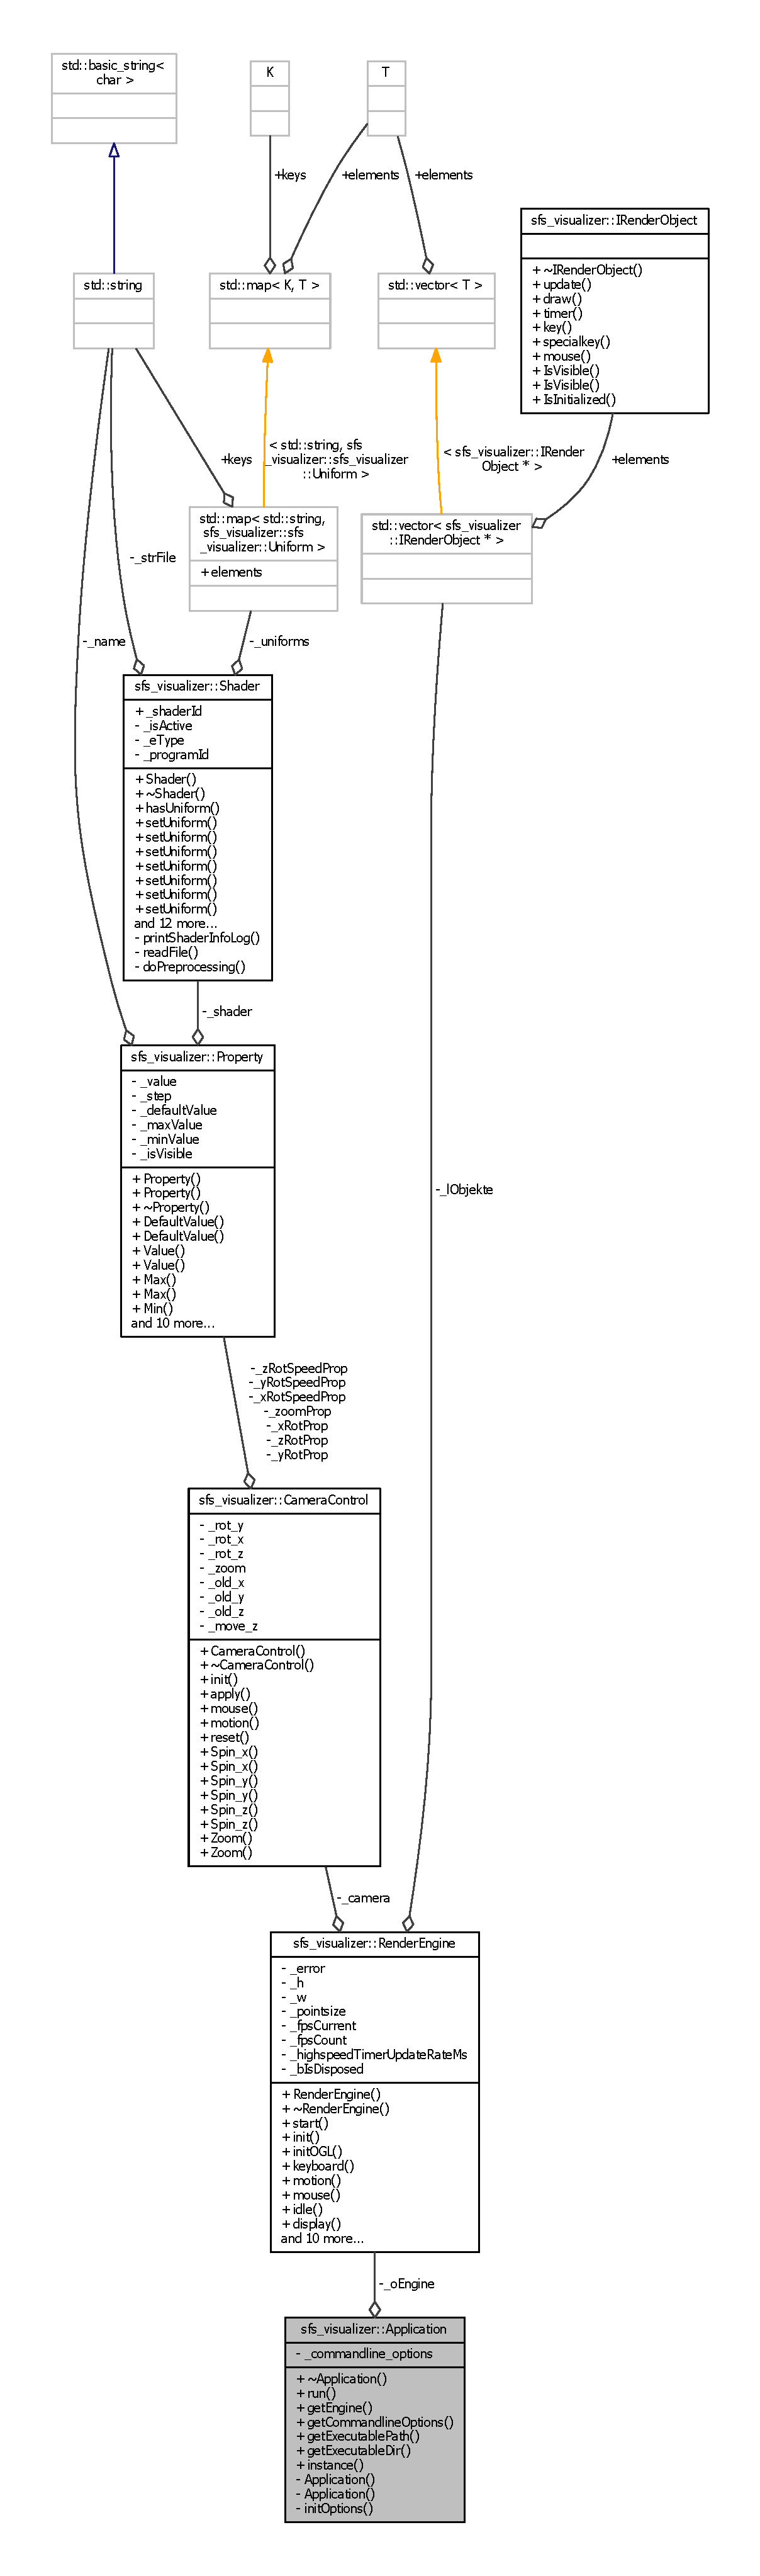
\includegraphics[height=550pt]{df/d88/classsfs__visualizer_1_1Application__coll__graph}
\end{center}
\end{figure}
\subsection*{Public Member Functions}
\begin{DoxyCompactItemize}
\item 
int {\bfseries run} (int ac, char $\ast$av[$\,$])\label{classsfs__visualizer_1_1Application_a5f172b387d5648986635a834671e15f7}

\item 
{\bf Render\-Engine} \& {\bfseries get\-Engine} ()\label{classsfs__visualizer_1_1Application_a1f03d282be02b67e743eb86c076905e3}

\item 
boost\-::program\-\_\-options\-::variables\-\_\-map {\bfseries get\-Commandline\-Options} () const \label{classsfs__visualizer_1_1Application_a2b70cdd8da81e2d73293b01c3125deae}

\item 
std\-::string {\bfseries get\-Executable\-Path} () const \label{classsfs__visualizer_1_1Application_a25a259c095c21540ba549cd8c0cb34ef}

\item 
std\-::string {\bfseries get\-Executable\-Dir} () const \label{classsfs__visualizer_1_1Application_a73d64fa96147de7b7b468b0e9fb19559}

\end{DoxyCompactItemize}
\subsection*{Static Public Member Functions}
\begin{DoxyCompactItemize}
\item 
static {\bf Application} \& {\bfseries instance} ()\label{classsfs__visualizer_1_1Application_ada3b7951bef34e1e6de30403eee8eada}

\end{DoxyCompactItemize}
\subsection*{Private Member Functions}
\begin{DoxyCompactItemize}
\item 
{\bfseries Application} (const {\bf Application} \&)\label{classsfs__visualizer_1_1Application_aae762bb7090da2e1db755d73f972c3be}

\item 
void {\bfseries init\-Options} (int ac, char $\ast$av[$\,$])\label{classsfs__visualizer_1_1Application_a6cf521cbce36f0ac4647470e53aaba40}

\end{DoxyCompactItemize}
\subsection*{Private Attributes}
\begin{DoxyCompactItemize}
\item 
{\bf Render\-Engine} {\bfseries \-\_\-o\-Engine}\label{classsfs__visualizer_1_1Application_aa97d6334e9169ab95984985e776cfbf1}

\item 
boost\-::program\-\_\-options\-::variables\-\_\-map {\bfseries \-\_\-commandline\-\_\-options}\label{classsfs__visualizer_1_1Application_a11a3f14eead7f89a6ec266571f90d0cc}

\end{DoxyCompactItemize}


\subsection{Detailed Description}


Definition at line 24 of file application.\-h.



The documentation for this class was generated from the following files\-:\begin{DoxyCompactItemize}
\item 
application.\-h\item 
application.\-cpp\end{DoxyCompactItemize}

\section{Application Class Reference}
\label{classApplication}\index{Application@{Application}}


{\ttfamily \#include $<$application.\-h$>$}



Collaboration diagram for Application\-:
\nopagebreak
\begin{figure}[H]
\begin{center}
\leavevmode
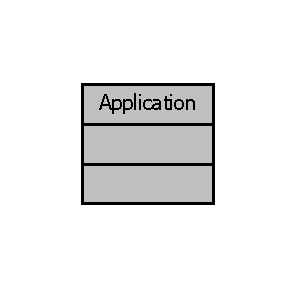
\includegraphics[width=142pt]{dd/d78/classApplication__coll__graph}
\end{center}
\end{figure}


\subsection{Detailed Description}
\begin{DoxyAuthor}{Author}
Marcus Zepp
\end{DoxyAuthor}
\begin{DoxyVersion}{Version}

\end{DoxyVersion}
\begin{DoxyParagraph}{Revision\-:}
1.\-0 
\end{DoxyParagraph}


\begin{DoxyDate}{Date}

\end{DoxyDate}
\begin{DoxyParagraph}{Date\-:}
2014/03/26 14\-:16\-:20 
\end{DoxyParagraph}


Contact\-: {\tt zeppfisj@mailbox.\-tu-\/berlin.\-de} 

The documentation for this class was generated from the following file\-:\begin{DoxyCompactItemize}
\item 
application.\-h\end{DoxyCompactItemize}

\section{sfs\-\_\-visualizer\-:\-:Camera\-Control Class Reference}
\label{classsfs__visualizer_1_1CameraControl}\index{sfs\-\_\-visualizer\-::\-Camera\-Control@{sfs\-\_\-visualizer\-::\-Camera\-Control}}


An orthographic camera, with x-\/y-\/z-\/rotation and zoom in texturespace.  




{\ttfamily \#include $<$cameracontrol.\-h$>$}



Collaboration diagram for sfs\-\_\-visualizer\-:\-:Camera\-Control\-:\nopagebreak
\begin{figure}[H]
\begin{center}
\leavevmode
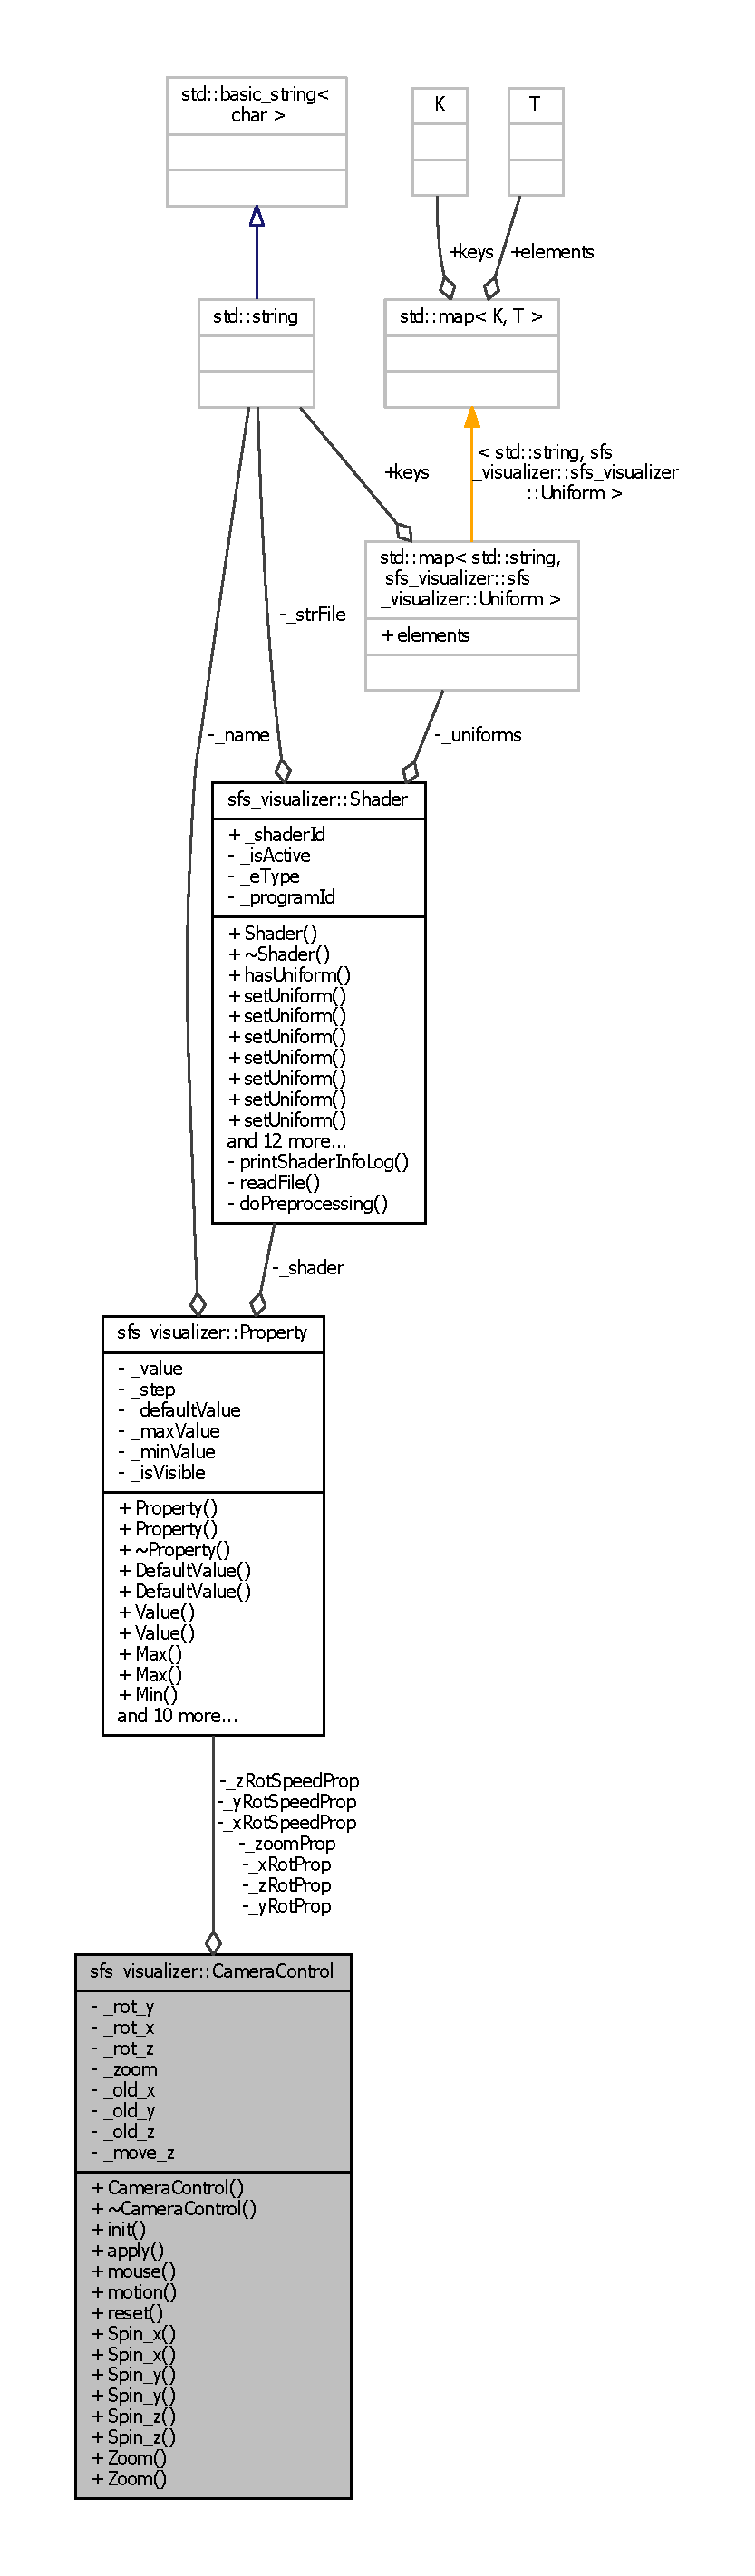
\includegraphics[height=550pt]{d8/d22/classsfs__visualizer_1_1CameraControl__coll__graph}
\end{center}
\end{figure}
\subsection*{Public Member Functions}
\begin{DoxyCompactItemize}
\item 
void {\bfseries init} (int width, int height)\label{classsfs__visualizer_1_1CameraControl_a2ebade4f88d9f8e2ef07b598be75165e}

\item 
void {\bfseries apply} ()\label{classsfs__visualizer_1_1CameraControl_a027eb280a548929964972a0269948704}

\item 
void {\bfseries mouse} (int button, int state, int x, int y)\label{classsfs__visualizer_1_1CameraControl_a763502cfb980553abf5ec46aa1c8547a}

\item 
void {\bfseries motion} (int x, int y)\label{classsfs__visualizer_1_1CameraControl_a91c42f259015cd609ed1c798648d2dc4}

\item 
void {\bfseries reset} ()\label{classsfs__visualizer_1_1CameraControl_aa79ef348ac442df65714a8d2a0e7cd12}

\item 
int {\bfseries Spin\-\_\-x} () const \label{classsfs__visualizer_1_1CameraControl_a2fafda6e38bdac37bbc46c4f1333040f}

\item 
void {\bfseries Spin\-\_\-x} (int val)\label{classsfs__visualizer_1_1CameraControl_a79adbf4e7dace42051c064968d4639fe}

\item 
int {\bfseries Spin\-\_\-y} () const \label{classsfs__visualizer_1_1CameraControl_a4da6283e846774916d071df453993eb0}

\item 
void {\bfseries Spin\-\_\-y} (int val)\label{classsfs__visualizer_1_1CameraControl_a0ded6da7a27228e8a4000d78508dc825}

\item 
int {\bfseries Spin\-\_\-z} () const \label{classsfs__visualizer_1_1CameraControl_aa72b99e4780eb1f62a83d6994fa3bdbb}

\item 
void {\bfseries Spin\-\_\-z} (int val)\label{classsfs__visualizer_1_1CameraControl_af98bf1747aa9cbcce19a96b78b7865b5}

\item 
int {\bfseries Zoom} () const \label{classsfs__visualizer_1_1CameraControl_a8b13370da1a6033ec63b46f79a1d056b}

\item 
void {\bfseries Zoom} (int val)\label{classsfs__visualizer_1_1CameraControl_ae09c78422ef19a9e3db08be0e9b13766}

\end{DoxyCompactItemize}
\subsection*{Private Attributes}
\begin{DoxyCompactItemize}
\item 
{\bf Property} \& {\bfseries \-\_\-x\-Rot\-Prop}\label{classsfs__visualizer_1_1CameraControl_a936c7501505965fe2cc85e7bdf98a66c}

\item 
{\bf Property} \& {\bfseries \-\_\-y\-Rot\-Prop}\label{classsfs__visualizer_1_1CameraControl_a523d6496d4368028f000244667515045}

\item 
{\bf Property} \& {\bfseries \-\_\-z\-Rot\-Prop}\label{classsfs__visualizer_1_1CameraControl_a6770009d7cd09b7a8cc6cf8dfc8e3a9f}

\item 
{\bf Property} \& {\bfseries \-\_\-x\-Rot\-Speed\-Prop}\label{classsfs__visualizer_1_1CameraControl_abed8587f59344d9f60c2f9b585388b1e}

\item 
{\bf Property} \& {\bfseries \-\_\-y\-Rot\-Speed\-Prop}\label{classsfs__visualizer_1_1CameraControl_a98e942491c2dbeff799b928f33949258}

\item 
{\bf Property} \& {\bfseries \-\_\-z\-Rot\-Speed\-Prop}\label{classsfs__visualizer_1_1CameraControl_a77143f7a759158fa4ca529df2c96f0aa}

\item 
{\bf Property} \& {\bfseries \-\_\-zoom\-Prop}\label{classsfs__visualizer_1_1CameraControl_a9f499e7a4351de5ce1110d342d117365}

\item 
int {\bfseries \-\_\-rot\-\_\-y}\label{classsfs__visualizer_1_1CameraControl_ad2e09efef85a9f2c11c368fb2b5a4340}

\item 
int {\bfseries \-\_\-rot\-\_\-x}\label{classsfs__visualizer_1_1CameraControl_adef736ee98d2b4a68f741521c9e51d30}

\item 
int {\bfseries \-\_\-rot\-\_\-z}\label{classsfs__visualizer_1_1CameraControl_aba1520613eee5bac18fe41face73ae60}

\item 
int {\bfseries \-\_\-zoom}\label{classsfs__visualizer_1_1CameraControl_a8d462a2cc5b46e4c7f4b25384e98b4a5}

\item 
int {\bfseries \-\_\-old\-\_\-x}\label{classsfs__visualizer_1_1CameraControl_afd2b2df2e93e7269863a887c5034c93a}

\item 
int {\bfseries \-\_\-old\-\_\-y}\label{classsfs__visualizer_1_1CameraControl_a43b01f73869123d8fd76eab0d5483bed}

\item 
int {\bfseries \-\_\-old\-\_\-z}\label{classsfs__visualizer_1_1CameraControl_ad29ecf67553a892ad19fbb2c50ea3848}

\item 
bool {\bfseries \-\_\-move\-\_\-z}\label{classsfs__visualizer_1_1CameraControl_af1b2a789e93bfa77ecc97f0214c8d7c5}

\end{DoxyCompactItemize}


\subsection{Detailed Description}
An orthographic camera, with x-\/y-\/z-\/rotation and zoom in texturespace. 

Definition at line 23 of file cameracontrol.\-h.



The documentation for this class was generated from the following files\-:\begin{DoxyCompactItemize}
\item 
cameracontrol.\-h\item 
cameracontrol.\-cpp\end{DoxyCompactItemize}

\section{Camera\-Control Class Reference}
\label{classCameraControl}\index{Camera\-Control@{Camera\-Control}}


{\ttfamily \#include $<$cameracontrol.\-h$>$}



Collaboration diagram for Camera\-Control\-:
\nopagebreak
\begin{figure}[H]
\begin{center}
\leavevmode
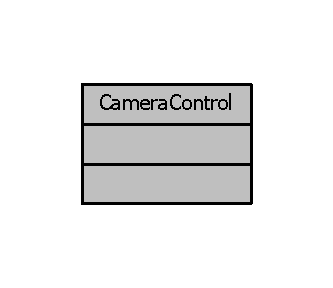
\includegraphics[width=160pt]{df/d8f/classCameraControl__coll__graph}
\end{center}
\end{figure}


\subsection{Detailed Description}
\begin{DoxyAuthor}{Author}
Marcus Zepp
\end{DoxyAuthor}
\begin{DoxyVersion}{Version}

\end{DoxyVersion}
\begin{DoxyParagraph}{Revision\-:}
1.\-0 
\end{DoxyParagraph}


\begin{DoxyDate}{Date}

\end{DoxyDate}
\begin{DoxyParagraph}{Date\-:}
2014/03/26 14\-:16\-:20 
\end{DoxyParagraph}


Contact\-: {\tt zeppfisj@mailbox.\-tu-\/berlin.\-de} 

The documentation for this class was generated from the following file\-:\begin{DoxyCompactItemize}
\item 
cameracontrol.\-h\end{DoxyCompactItemize}

\section{sfs\-\_\-visualizer\-:\-:Colormap\-View Class Reference}
\label{classsfs__visualizer_1_1ColormapView}\index{sfs\-\_\-visualizer\-::\-Colormap\-View@{sfs\-\_\-visualizer\-::\-Colormap\-View}}


A Render\-Object, that displays the colormap on the screen.  




{\ttfamily \#include $<$colormapview.\-h$>$}



Inheritance diagram for sfs\-\_\-visualizer\-:\-:Colormap\-View\-:\nopagebreak
\begin{figure}[H]
\begin{center}
\leavevmode
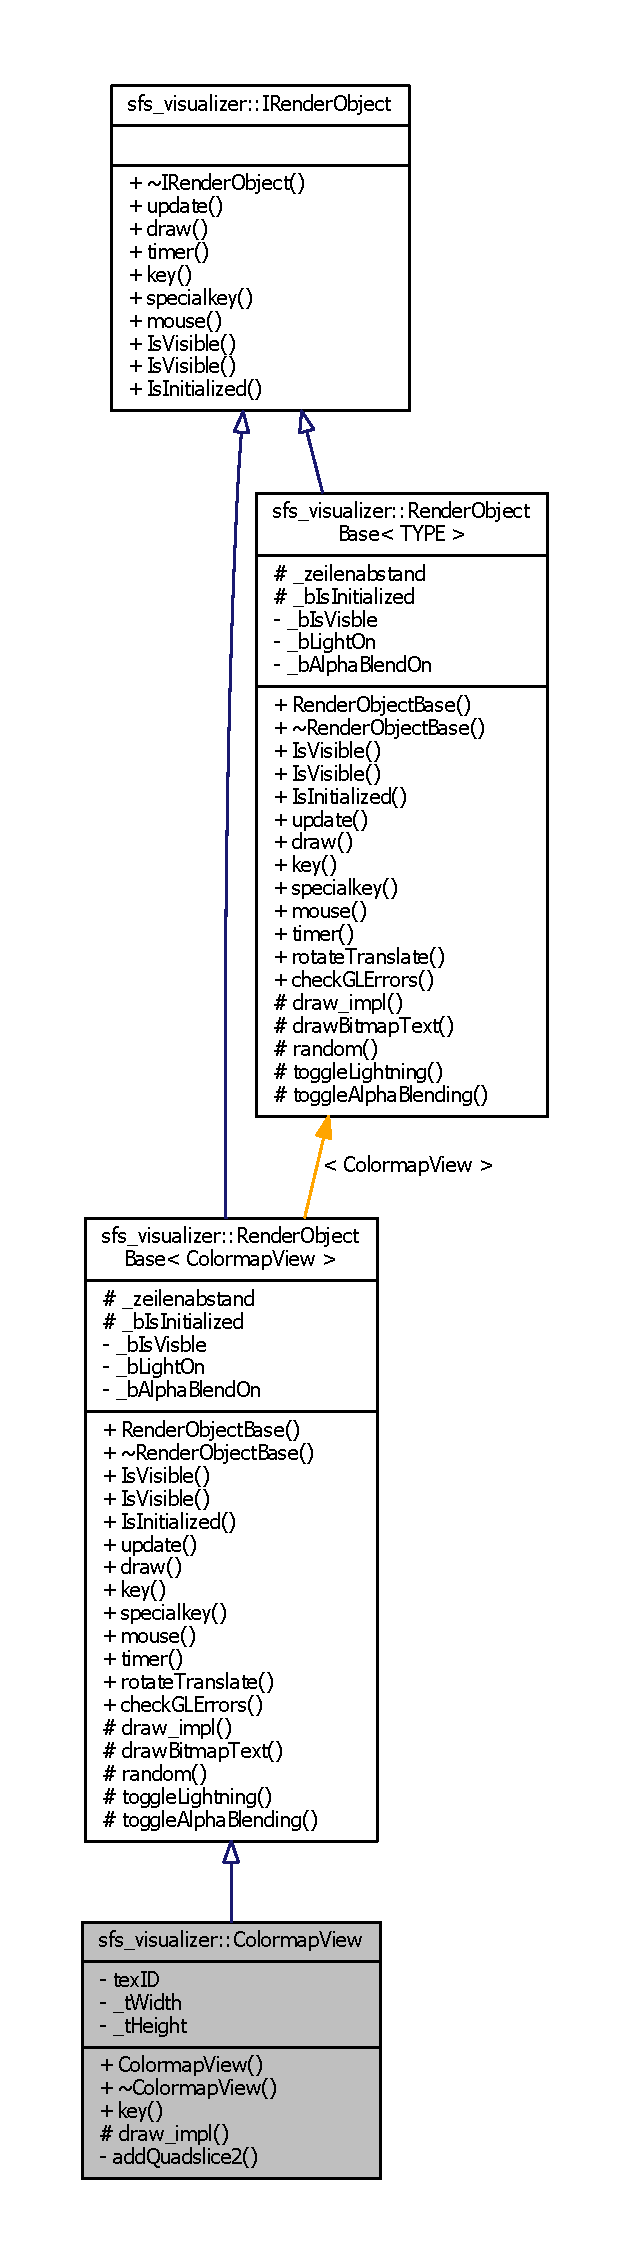
\includegraphics[height=550pt]{da/db7/classsfs__visualizer_1_1ColormapView__inherit__graph}
\end{center}
\end{figure}


Collaboration diagram for sfs\-\_\-visualizer\-:\-:Colormap\-View\-:\nopagebreak
\begin{figure}[H]
\begin{center}
\leavevmode
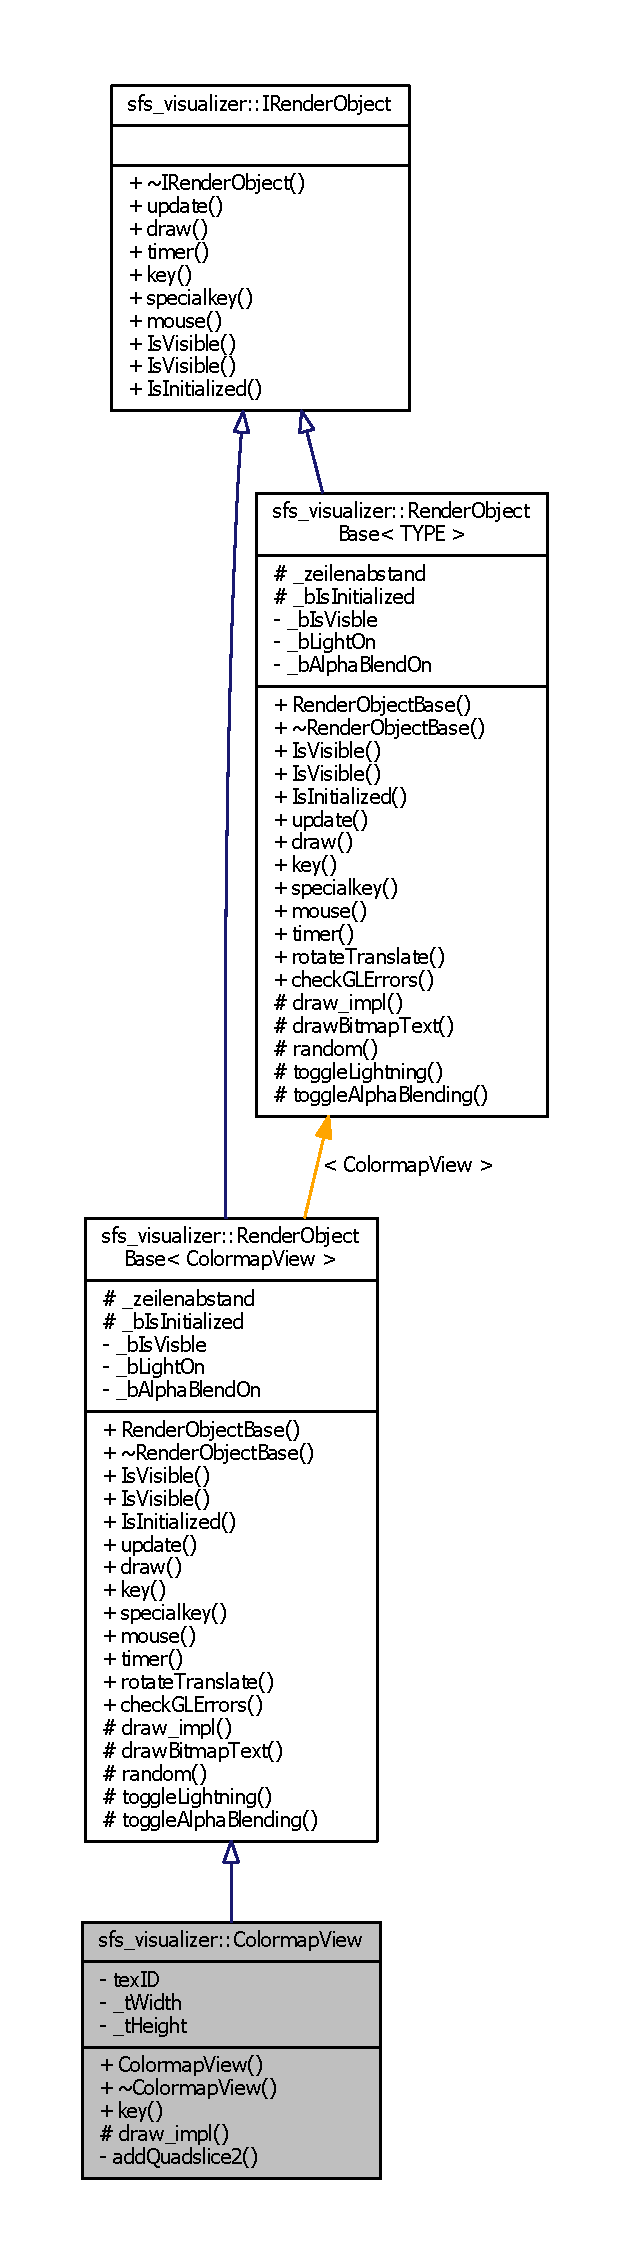
\includegraphics[height=550pt]{de/d8a/classsfs__visualizer_1_1ColormapView__coll__graph}
\end{center}
\end{figure}
\subsection*{Public Member Functions}
\begin{DoxyCompactItemize}
\item 
virtual void {\bf key} (unsigned char key, int x, int y)
\begin{DoxyCompactList}\small\item\em user inputs \end{DoxyCompactList}\end{DoxyCompactItemize}
\subsection*{Protected Member Functions}
\begin{DoxyCompactItemize}
\item 
virtual void {\bfseries draw\-\_\-impl} ()\label{classsfs__visualizer_1_1ColormapView_a952a51cc68b2e495ae26183e84178044}

\end{DoxyCompactItemize}
\subsection*{Private Member Functions}
\begin{DoxyCompactItemize}
\item 
void {\bfseries add\-Quadslice2} (float z\-Offset)\label{classsfs__visualizer_1_1ColormapView_a2d383483dc56ef33a3210acabab9b843}

\end{DoxyCompactItemize}
\subsection*{Private Attributes}
\begin{DoxyCompactItemize}
\item 
int {\bfseries tex\-I\-D}\label{classsfs__visualizer_1_1ColormapView_a4384eaf9f23f426942ca99a73bd2b40b}

\item 
G\-Lint {\bfseries \-\_\-t\-Width}\label{classsfs__visualizer_1_1ColormapView_a9e987f1890756015a8ec5ca9f5de5a10}

\item 
G\-Lint {\bfseries \-\_\-t\-Height}\label{classsfs__visualizer_1_1ColormapView_a9b2ff0ca5394e85eebd64cc0ac44084b}

\end{DoxyCompactItemize}
\subsection*{Additional Inherited Members}


\subsection{Detailed Description}
A Render\-Object, that displays the colormap on the screen. 

Definition at line 24 of file colormapview.\-h.



\subsection{Member Function Documentation}
\index{sfs\-\_\-visualizer\-::\-Colormap\-View@{sfs\-\_\-visualizer\-::\-Colormap\-View}!key@{key}}
\index{key@{key}!sfs_visualizer::ColormapView@{sfs\-\_\-visualizer\-::\-Colormap\-View}}
\subsubsection[{key}]{\setlength{\rightskip}{0pt plus 5cm}void Colormap\-View\-::key (
\begin{DoxyParamCaption}
\item[{unsigned char}]{key, }
\item[{int}]{x, }
\item[{int}]{y}
\end{DoxyParamCaption}
)\hspace{0.3cm}{\ttfamily [virtual]}}\label{classsfs__visualizer_1_1ColormapView_af9381d745eb32e41fbc588cb325ffe4c}


user inputs 



Reimplemented from {\bf sfs\-\_\-visualizer\-::\-Render\-Object\-Base$<$ Colormap\-View $>$} \doxyref{}{p.}{de/d2a/classsfs__visualizer_1_1RenderObjectBase_a3f0106a0ce3861f34e5330da65e7bdd4}.



Definition at line 31 of file colormapview.\-cpp.



References sfs\-\_\-visualizer\-::\-Render\-Object\-Base$<$ Colormap\-View $>$\-::\-Is\-Visible().



The documentation for this class was generated from the following files\-:\begin{DoxyCompactItemize}
\item 
colormapview.\-h\item 
colormapview.\-cpp\end{DoxyCompactItemize}

\section{Colormap\-View Class Reference}
\label{classColormapView}\index{Colormap\-View@{Colormap\-View}}


{\ttfamily \#include $<$colormapview.\-h$>$}



Collaboration diagram for Colormap\-View\-:
\nopagebreak
\begin{figure}[H]
\begin{center}
\leavevmode
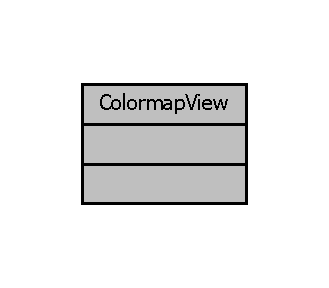
\includegraphics[width=158pt]{d5/da7/classColormapView__coll__graph}
\end{center}
\end{figure}


\subsection{Detailed Description}
\begin{DoxyAuthor}{Author}
Marcus Zepp
\end{DoxyAuthor}
\begin{DoxyVersion}{Version}

\end{DoxyVersion}
\begin{DoxyParagraph}{Revision\-:}
1.\-0 
\end{DoxyParagraph}


\begin{DoxyDate}{Date}

\end{DoxyDate}
\begin{DoxyParagraph}{Date\-:}
2014/03/26 14\-:16\-:20 
\end{DoxyParagraph}


Contact\-: {\tt zeppfisj@mailbox.\-tu-\/berlin.\-de} 

The documentation for this class was generated from the following file\-:\begin{DoxyCompactItemize}
\item 
colormapview.\-h\end{DoxyCompactItemize}

\section{sfs\-\_\-visualizer\-:\-:Command Class Reference}
\label{classsfs__visualizer_1_1Command}\index{sfs\-\_\-visualizer\-::\-Command@{sfs\-\_\-visualizer\-::\-Command}}


implements the command-\/pattern, that abstracts actions, that can be executed  




{\ttfamily \#include $<$command.\-h$>$}



Inheritance diagram for sfs\-\_\-visualizer\-:\-:Command\-:\nopagebreak
\begin{figure}[H]
\begin{center}
\leavevmode
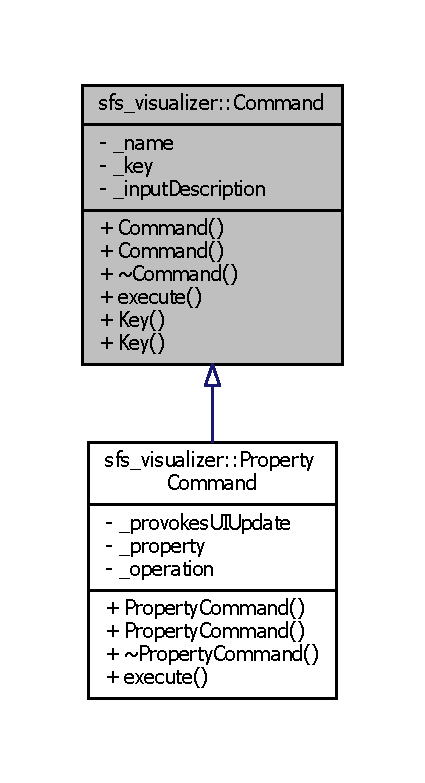
\includegraphics[width=204pt]{d4/d10/classsfs__visualizer_1_1Command__inherit__graph}
\end{center}
\end{figure}


Collaboration diagram for sfs\-\_\-visualizer\-:\-:Command\-:\nopagebreak
\begin{figure}[H]
\begin{center}
\leavevmode
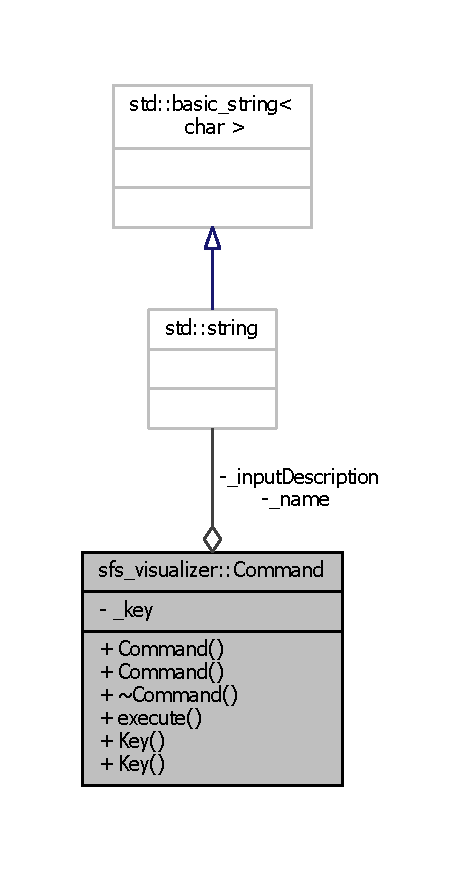
\includegraphics[width=223pt]{d9/dc6/classsfs__visualizer_1_1Command__coll__graph}
\end{center}
\end{figure}
\subsection*{Public Member Functions}
\begin{DoxyCompactItemize}
\item 
{\bfseries Command} (unsigned char key, const std\-::string \&input\-Description, const std\-::string \&name)\label{classsfs__visualizer_1_1Command_ae2614111a870d6f6cc5aaecdd78db126}

\item 
virtual bool {\bfseries execute} ()=0\label{classsfs__visualizer_1_1Command_a5d2f2897ed6d2a517034cc9f39573473}

\item 
char {\bfseries Key} () const \label{classsfs__visualizer_1_1Command_a536fba3a4a60b98a3fbe4f9f408a704c}

\item 
void {\bfseries Key} (char val)\label{classsfs__visualizer_1_1Command_a6783c6e3be00bafa41a4fd8c5e2afcfe}

\end{DoxyCompactItemize}
\subsection*{Private Attributes}
\begin{DoxyCompactItemize}
\item 
std\-::string {\bfseries \-\_\-name}\label{classsfs__visualizer_1_1Command_a11380d564fe5f57be44a65a4b7c86ad7}

\item 
unsigned char {\bfseries \-\_\-key}\label{classsfs__visualizer_1_1Command_a47117c28736e509c1c6a8744b9e4f1bd}

\item 
std\-::string {\bfseries \-\_\-input\-Description}\label{classsfs__visualizer_1_1Command_afe2999f3f0368ad50d5052156d90ec68}

\end{DoxyCompactItemize}


\subsection{Detailed Description}
implements the command-\/pattern, that abstracts actions, that can be executed 

Definition at line 26 of file command.\-h.



The documentation for this class was generated from the following files\-:\begin{DoxyCompactItemize}
\item 
command.\-h\item 
command.\-cpp\end{DoxyCompactItemize}

\section{Command Class Reference}
\label{classCommand}\index{Command@{Command}}


{\ttfamily \#include $<$command.\-h$>$}



Collaboration diagram for Command\-:
\nopagebreak
\begin{figure}[H]
\begin{center}
\leavevmode
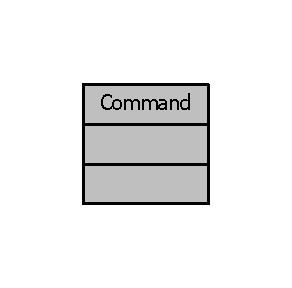
\includegraphics[width=140pt]{df/d45/classCommand__coll__graph}
\end{center}
\end{figure}


\subsection{Detailed Description}
\begin{DoxyAuthor}{Author}
Marcus Zepp
\end{DoxyAuthor}
\begin{DoxyVersion}{Version}

\end{DoxyVersion}
\begin{DoxyParagraph}{Revision\-:}
1.\-0 
\end{DoxyParagraph}


\begin{DoxyDate}{Date}

\end{DoxyDate}
\begin{DoxyParagraph}{Date\-:}
2014/03/26 14\-:16\-:20 
\end{DoxyParagraph}


Contact\-: {\tt zeppfisj@mailbox.\-tu-\/berlin.\-de} 

The documentation for this class was generated from the following file\-:\begin{DoxyCompactItemize}
\item 
command.\-h\end{DoxyCompactItemize}

\section{sfs\-\_\-visualizer\-:\-:Command\-Manager Class Reference}
\label{classsfs__visualizer_1_1CommandManager}\index{sfs\-\_\-visualizer\-::\-Command\-Manager@{sfs\-\_\-visualizer\-::\-Command\-Manager}}


this class knows all commands and can dispatch userinputs to them  




{\ttfamily \#include $<$commandmanager.\-h$>$}



Collaboration diagram for sfs\-\_\-visualizer\-:\-:Command\-Manager\-:\nopagebreak
\begin{figure}[H]
\begin{center}
\leavevmode
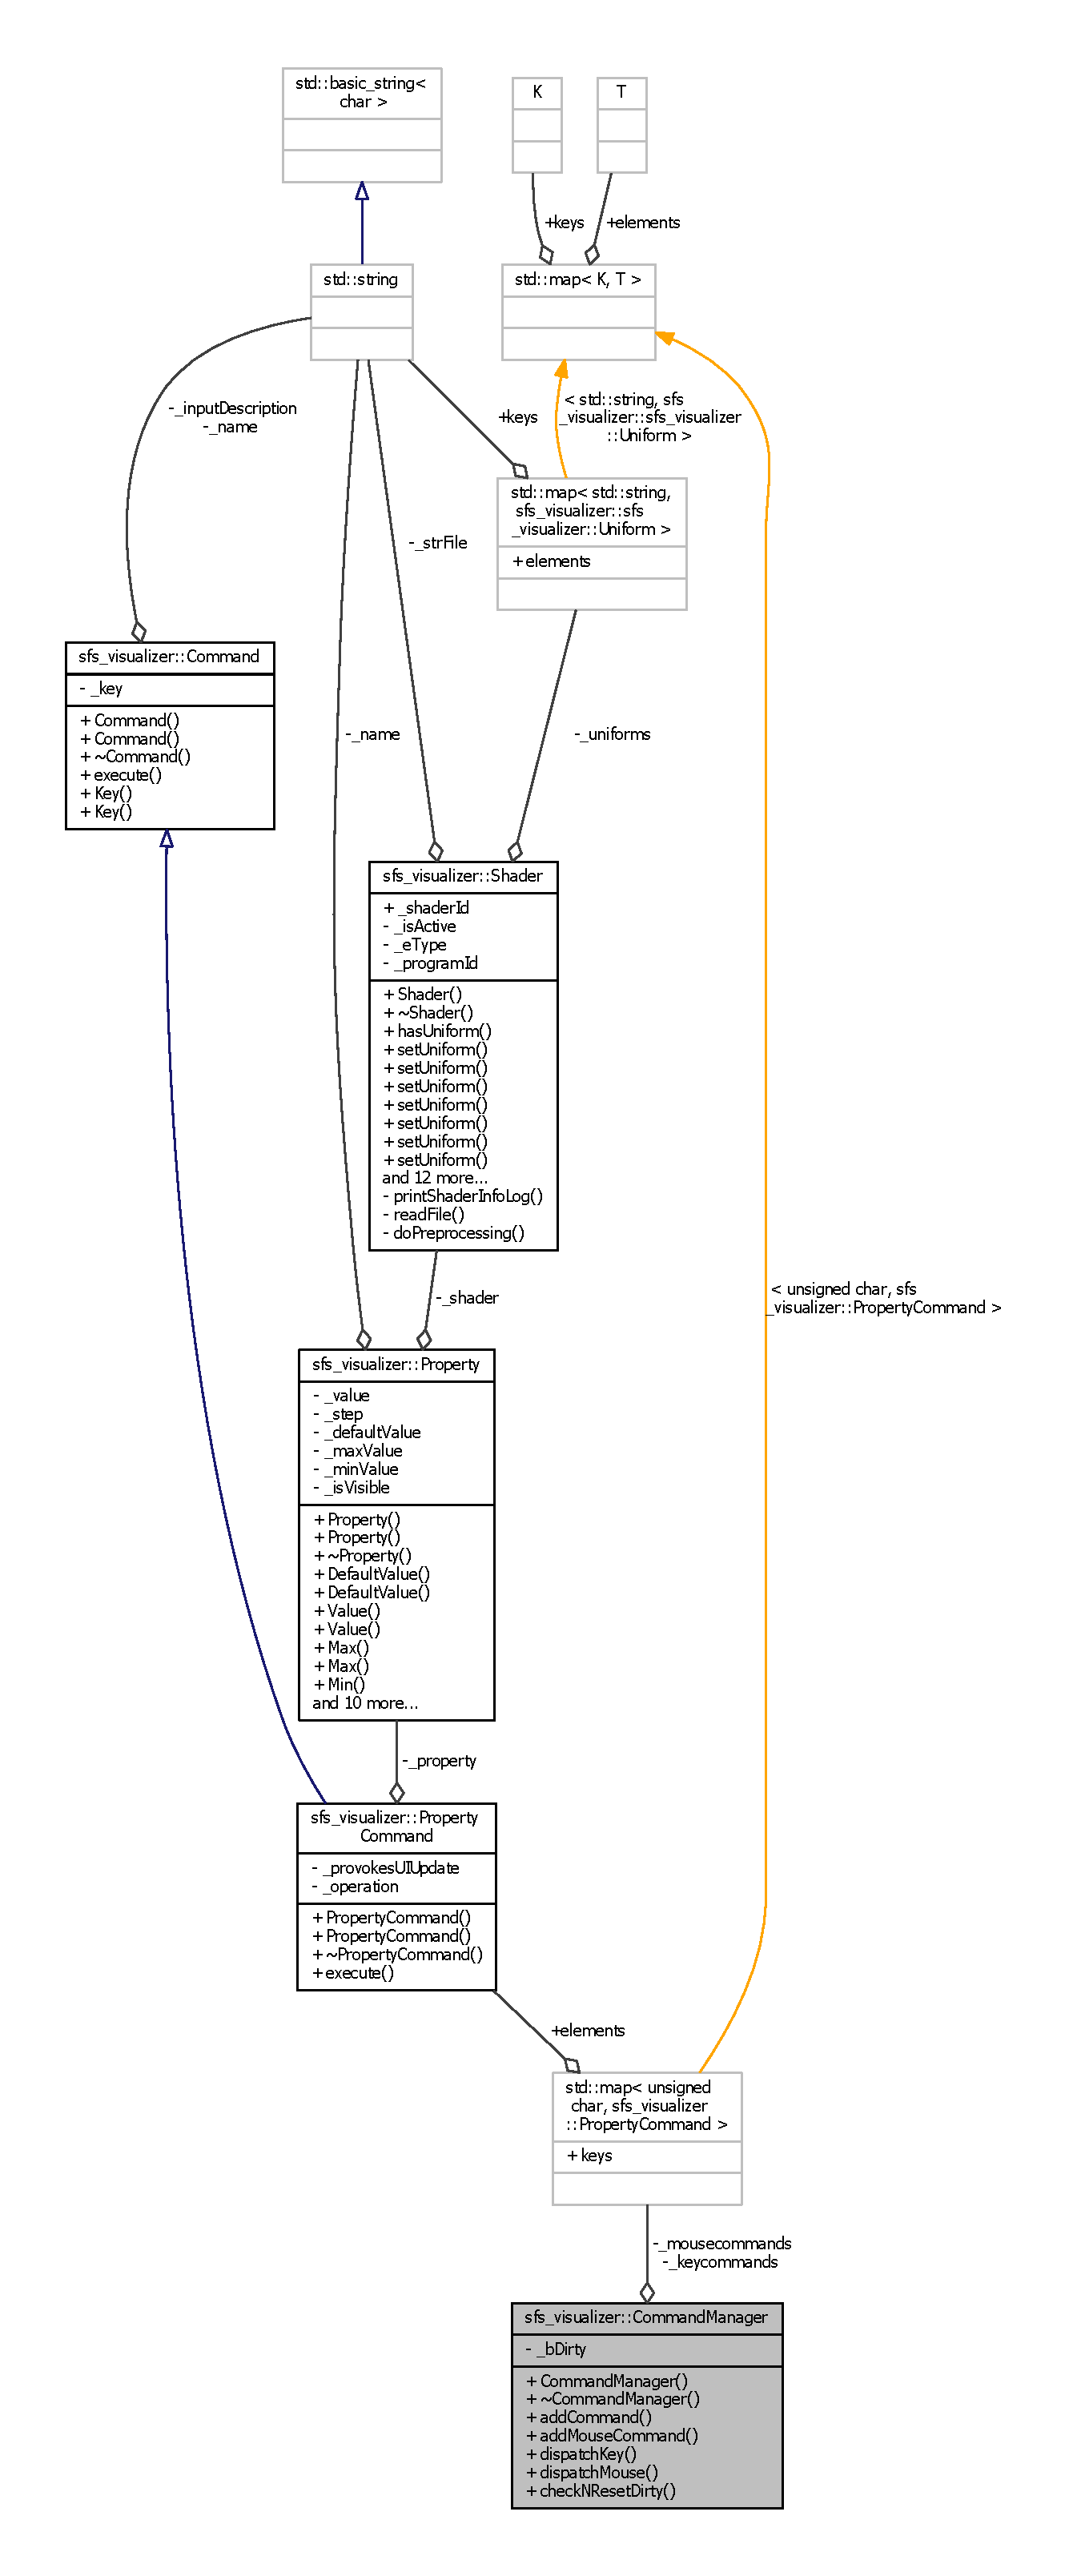
\includegraphics[height=550pt]{da/d3f/classsfs__visualizer_1_1CommandManager__coll__graph}
\end{center}
\end{figure}
\subsection*{Public Member Functions}
\begin{DoxyCompactItemize}
\item 
void {\bfseries add\-Command} (const std\-::string \&name, unsigned char key, const std\-::string \&input\-Description, {\bf Property} \&prop, Property\-Command\-::\-Operation operation, bool provokes\-U\-I\-Update=true)\label{classsfs__visualizer_1_1CommandManager_a095b9ca729812dc23abd0f3bf9036dc4}

\item 
void {\bfseries add\-Mouse\-Command} (const std\-::string \&name, unsigned char key, const std\-::string \&input\-Description, {\bf Property} \&prop, Property\-Command\-::\-Operation operation, bool provokes\-U\-I\-Update=true)\label{classsfs__visualizer_1_1CommandManager_ab68861e23d76b02f3bc18695ef7374dd}

\item 
void {\bfseries dispatch\-Key} (unsigned char key)\label{classsfs__visualizer_1_1CommandManager_a0df8c9aca76da88b8ea6878b3bdea3ff}

\item 
void {\bfseries dispatch\-Mouse} (unsigned char key)\label{classsfs__visualizer_1_1CommandManager_a01593421c259a5711a54a2cbde85d494}

\item 
bool {\bfseries check\-N\-Reset\-Dirty} ()\label{classsfs__visualizer_1_1CommandManager_a78df62b34b26990ac74eaf8f565465d4}

\end{DoxyCompactItemize}
\subsection*{Private Attributes}
\begin{DoxyCompactItemize}
\item 
bool {\bfseries \-\_\-b\-Dirty}\label{classsfs__visualizer_1_1CommandManager_afe91bb38d7a8e4d4648c5cd6b163a8f5}

\item 
std\-::map$<$ unsigned char, \\*
{\bf Property\-Command} $>$ {\bfseries \-\_\-keycommands}\label{classsfs__visualizer_1_1CommandManager_a5b254603d1ced0330d437bab4ebed23a}

\item 
std\-::map$<$ unsigned char, \\*
{\bf Property\-Command} $>$ {\bfseries \-\_\-mousecommands}\label{classsfs__visualizer_1_1CommandManager_a9ec682196453e50cd7c0e32d777951ae}

\end{DoxyCompactItemize}


\subsection{Detailed Description}
this class knows all commands and can dispatch userinputs to them 

Definition at line 25 of file commandmanager.\-h.



The documentation for this class was generated from the following files\-:\begin{DoxyCompactItemize}
\item 
commandmanager.\-h\item 
commandmanager.\-cpp\end{DoxyCompactItemize}

\section{Command\-Manager Class Reference}
\label{classCommandManager}\index{Command\-Manager@{Command\-Manager}}


{\ttfamily \#include $<$commandmanager.\-h$>$}



Collaboration diagram for Command\-Manager\-:
\nopagebreak
\begin{figure}[H]
\begin{center}
\leavevmode
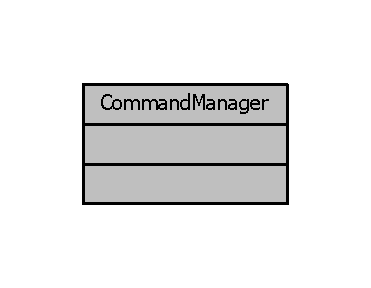
\includegraphics[width=178pt]{d3/d21/classCommandManager__coll__graph}
\end{center}
\end{figure}


\subsection{Detailed Description}
\begin{DoxyAuthor}{Author}
Marcus Zepp
\end{DoxyAuthor}
\begin{DoxyVersion}{Version}

\end{DoxyVersion}
\begin{DoxyParagraph}{Revision\-:}
1.\-0 
\end{DoxyParagraph}


\begin{DoxyDate}{Date}

\end{DoxyDate}
\begin{DoxyParagraph}{Date\-:}
2014/03/26 14\-:16\-:20 
\end{DoxyParagraph}


Contact\-: {\tt zeppfisj@mailbox.\-tu-\/berlin.\-de} 

The documentation for this class was generated from the following file\-:\begin{DoxyCompactItemize}
\item 
commandmanager.\-h\end{DoxyCompactItemize}

\section{sfs\-\_\-visualizer\-:\-:Coordinate\-System Class Reference}
\label{classsfs__visualizer_1_1CoordinateSystem}\index{sfs\-\_\-visualizer\-::\-Coordinate\-System@{sfs\-\_\-visualizer\-::\-Coordinate\-System}}


A Render\-Object, that displays a coordinate system on the screen.  




{\ttfamily \#include $<$coordinatesystem.\-h$>$}



Inheritance diagram for sfs\-\_\-visualizer\-:\-:Coordinate\-System\-:\nopagebreak
\begin{figure}[H]
\begin{center}
\leavevmode
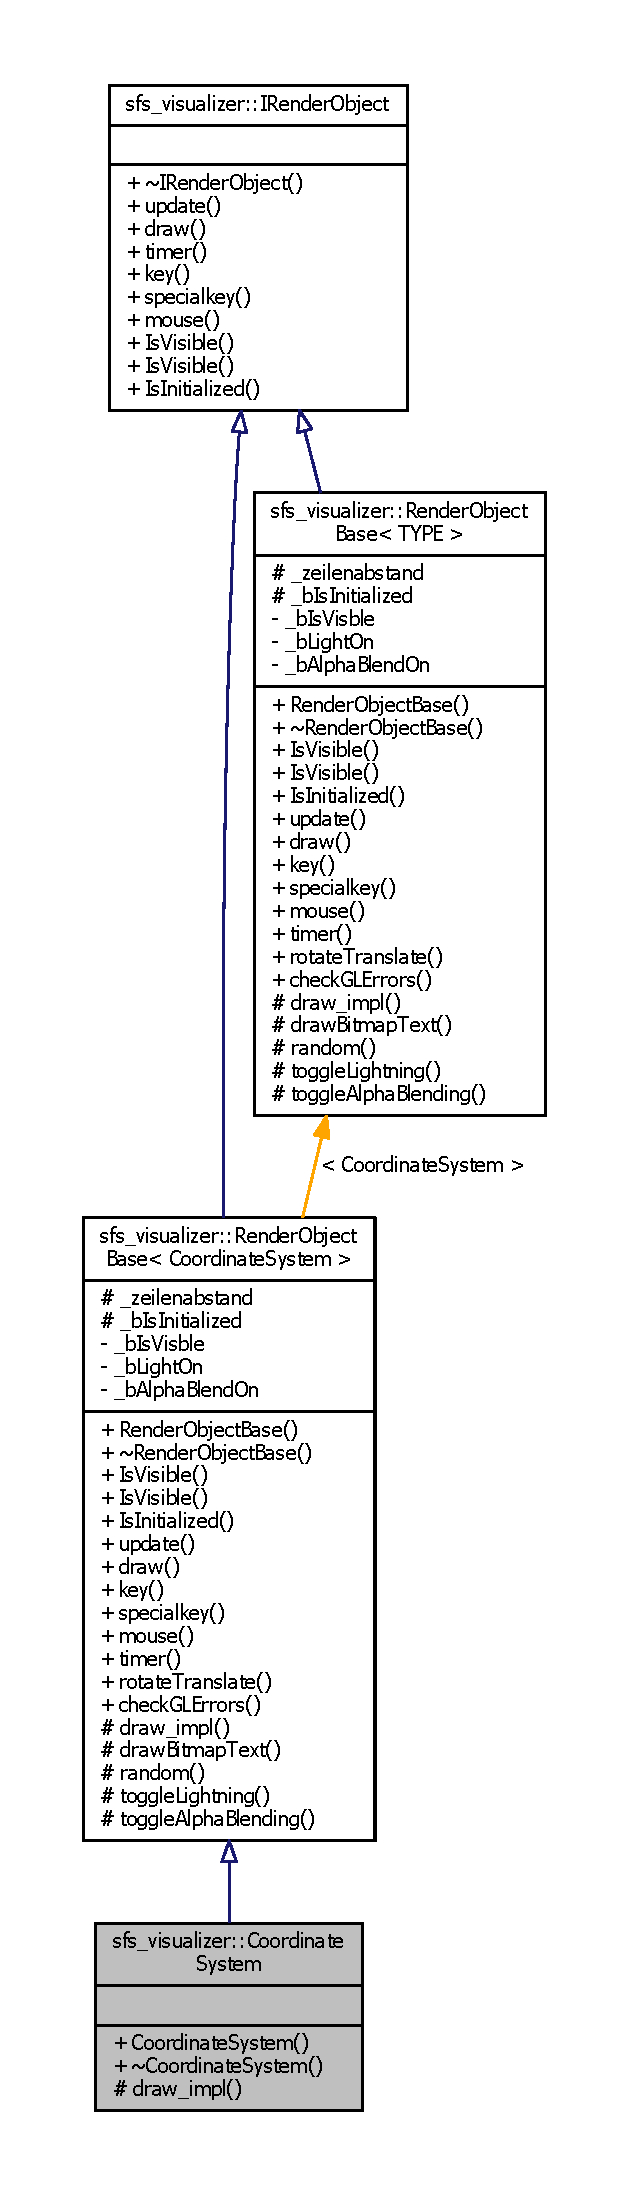
\includegraphics[height=550pt]{d7/d9c/classsfs__visualizer_1_1CoordinateSystem__inherit__graph}
\end{center}
\end{figure}


Collaboration diagram for sfs\-\_\-visualizer\-:\-:Coordinate\-System\-:\nopagebreak
\begin{figure}[H]
\begin{center}
\leavevmode
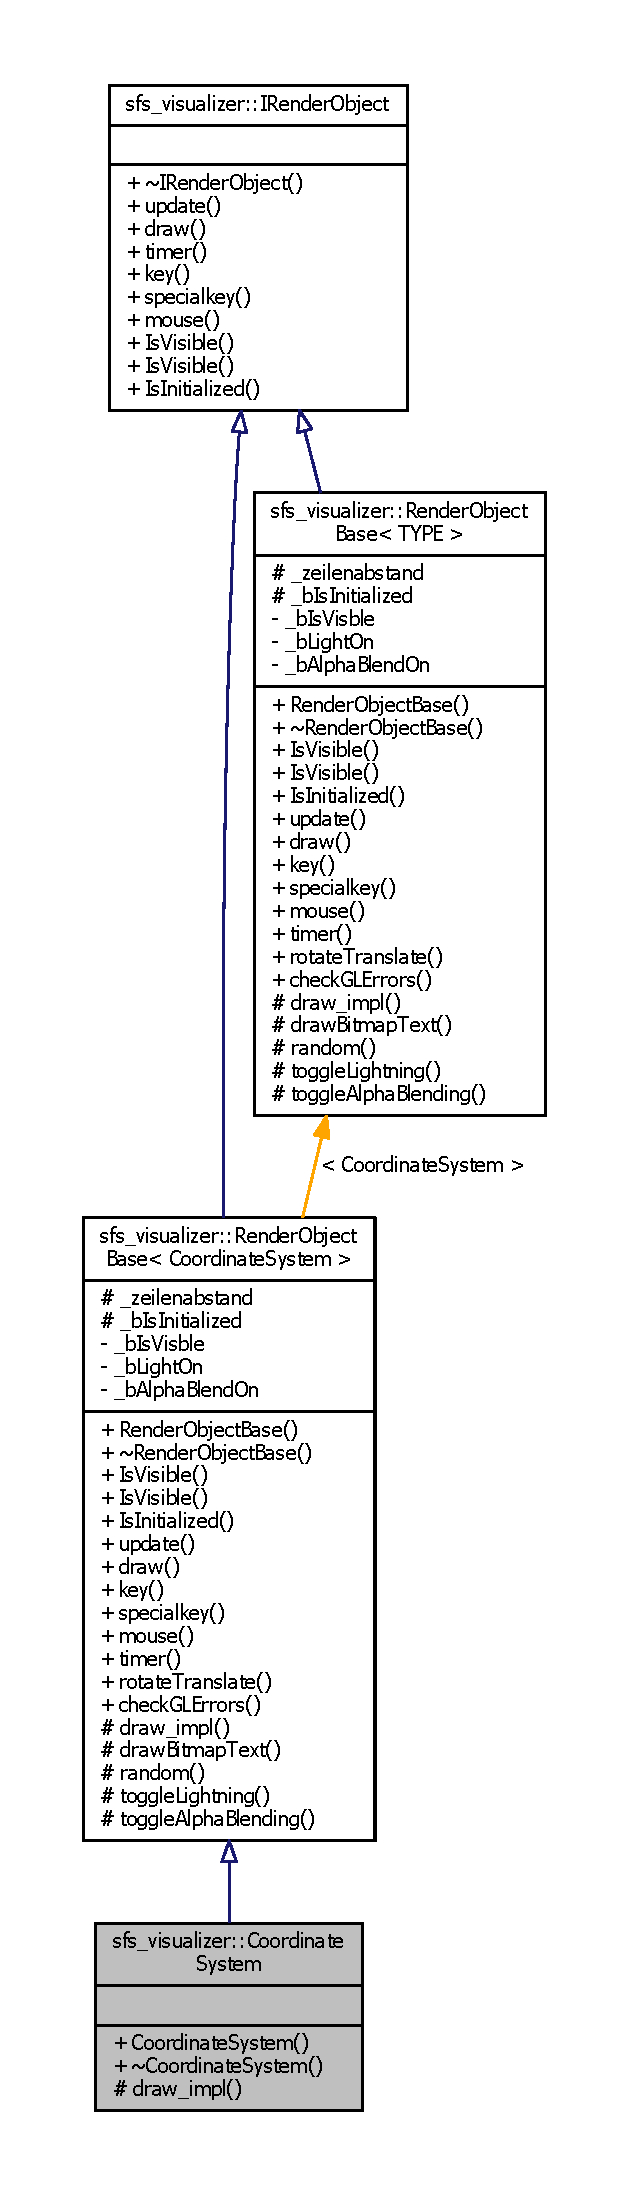
\includegraphics[height=550pt]{d9/dd6/classsfs__visualizer_1_1CoordinateSystem__coll__graph}
\end{center}
\end{figure}
\subsection*{Protected Member Functions}
\begin{DoxyCompactItemize}
\item 
virtual void {\bfseries draw\-\_\-impl} ()\label{classsfs__visualizer_1_1CoordinateSystem_ad224ce35719deaee49250db24da0fd08}

\end{DoxyCompactItemize}
\subsection*{Additional Inherited Members}


\subsection{Detailed Description}
A Render\-Object, that displays a coordinate system on the screen. 

Definition at line 24 of file coordinatesystem.\-h.



The documentation for this class was generated from the following files\-:\begin{DoxyCompactItemize}
\item 
coordinatesystem.\-h\item 
coordinatesystem.\-cpp\end{DoxyCompactItemize}

\section{Coordinate\-System Class Reference}
\label{classCoordinateSystem}\index{Coordinate\-System@{Coordinate\-System}}


{\ttfamily \#include $<$coordinatesystem.\-h$>$}



Collaboration diagram for Coordinate\-System\-:
\nopagebreak
\begin{figure}[H]
\begin{center}
\leavevmode
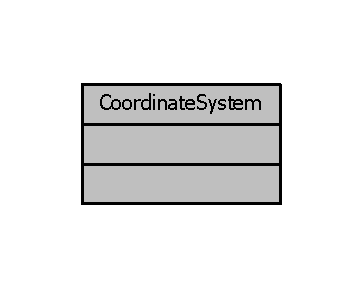
\includegraphics[width=174pt]{d7/d07/classCoordinateSystem__coll__graph}
\end{center}
\end{figure}


\subsection{Detailed Description}
\begin{DoxyAuthor}{Author}
Marcus Zepp
\end{DoxyAuthor}
\begin{DoxyVersion}{Version}

\end{DoxyVersion}
\begin{DoxyParagraph}{Revision\-:}
1.\-0 
\end{DoxyParagraph}


\begin{DoxyDate}{Date}

\end{DoxyDate}
\begin{DoxyParagraph}{Date\-:}
2014/03/26 14\-:16\-:20 
\end{DoxyParagraph}


Contact\-: {\tt zeppfisj@mailbox.\-tu-\/berlin.\-de} 

The documentation for this class was generated from the following file\-:\begin{DoxyCompactItemize}
\item 
coordinatesystem.\-h\end{DoxyCompactItemize}

\section{Field\-Viewer\-Base Class Reference}
\label{classFieldViewerBase}\index{Field\-Viewer\-Base@{Field\-Viewer\-Base}}


{\ttfamily \#include $<$fieldviewerbase.\-h$>$}



Collaboration diagram for Field\-Viewer\-Base\-:
\nopagebreak
\begin{figure}[H]
\begin{center}
\leavevmode
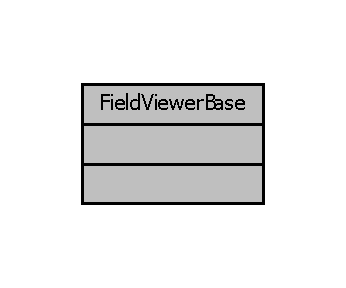
\includegraphics[width=166pt]{dd/df7/classFieldViewerBase__coll__graph}
\end{center}
\end{figure}


\subsection{Detailed Description}
\begin{DoxyAuthor}{Author}
Marcus Zepp
\end{DoxyAuthor}
\begin{DoxyVersion}{Version}

\end{DoxyVersion}
\begin{DoxyParagraph}{Revision\-:}
1.\-0 
\end{DoxyParagraph}


\begin{DoxyDate}{Date}

\end{DoxyDate}
\begin{DoxyParagraph}{Date\-:}
2014/03/26 14\-:16\-:20 
\end{DoxyParagraph}


Contact\-: {\tt zeppfisj@mailbox.\-tu-\/berlin.\-de} 

The documentation for this class was generated from the following file\-:\begin{DoxyCompactItemize}
\item 
fieldviewerbase.\-h\end{DoxyCompactItemize}

\section{sfs\-\_\-visualizer\-:\-:Field\-Viewer\-Base Class Reference}
\label{classsfs__visualizer_1_1FieldViewerBase}\index{sfs\-\_\-visualizer\-::\-Field\-Viewer\-Base@{sfs\-\_\-visualizer\-::\-Field\-Viewer\-Base}}


A Base class for classes that can show soundfields either with shearwarping or a raytracer.  




{\ttfamily \#include $<$fieldviewerbase.\-h$>$}



Inheritance diagram for sfs\-\_\-visualizer\-:\-:Field\-Viewer\-Base\-:
\nopagebreak
\begin{figure}[H]
\begin{center}
\leavevmode
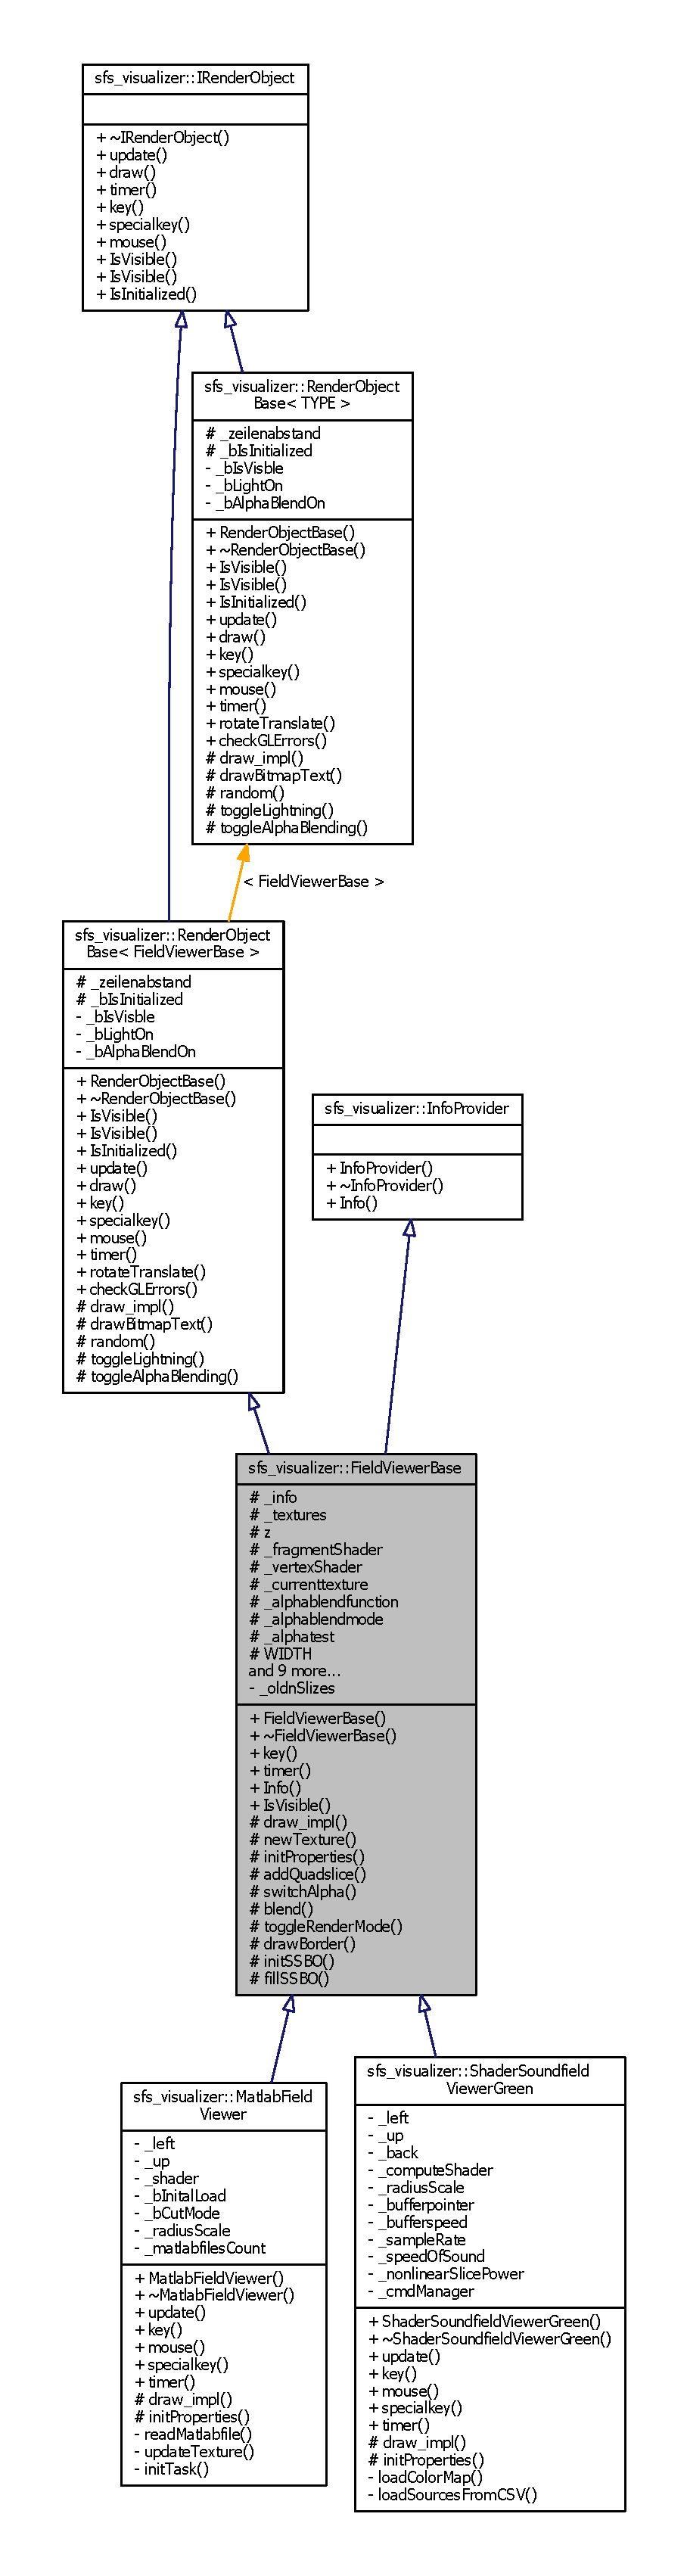
\includegraphics[height=550pt]{d8/da0/classsfs__visualizer_1_1FieldViewerBase__inherit__graph}
\end{center}
\end{figure}


Collaboration diagram for sfs\-\_\-visualizer\-:\-:Field\-Viewer\-Base\-:
\nopagebreak
\begin{figure}[H]
\begin{center}
\leavevmode
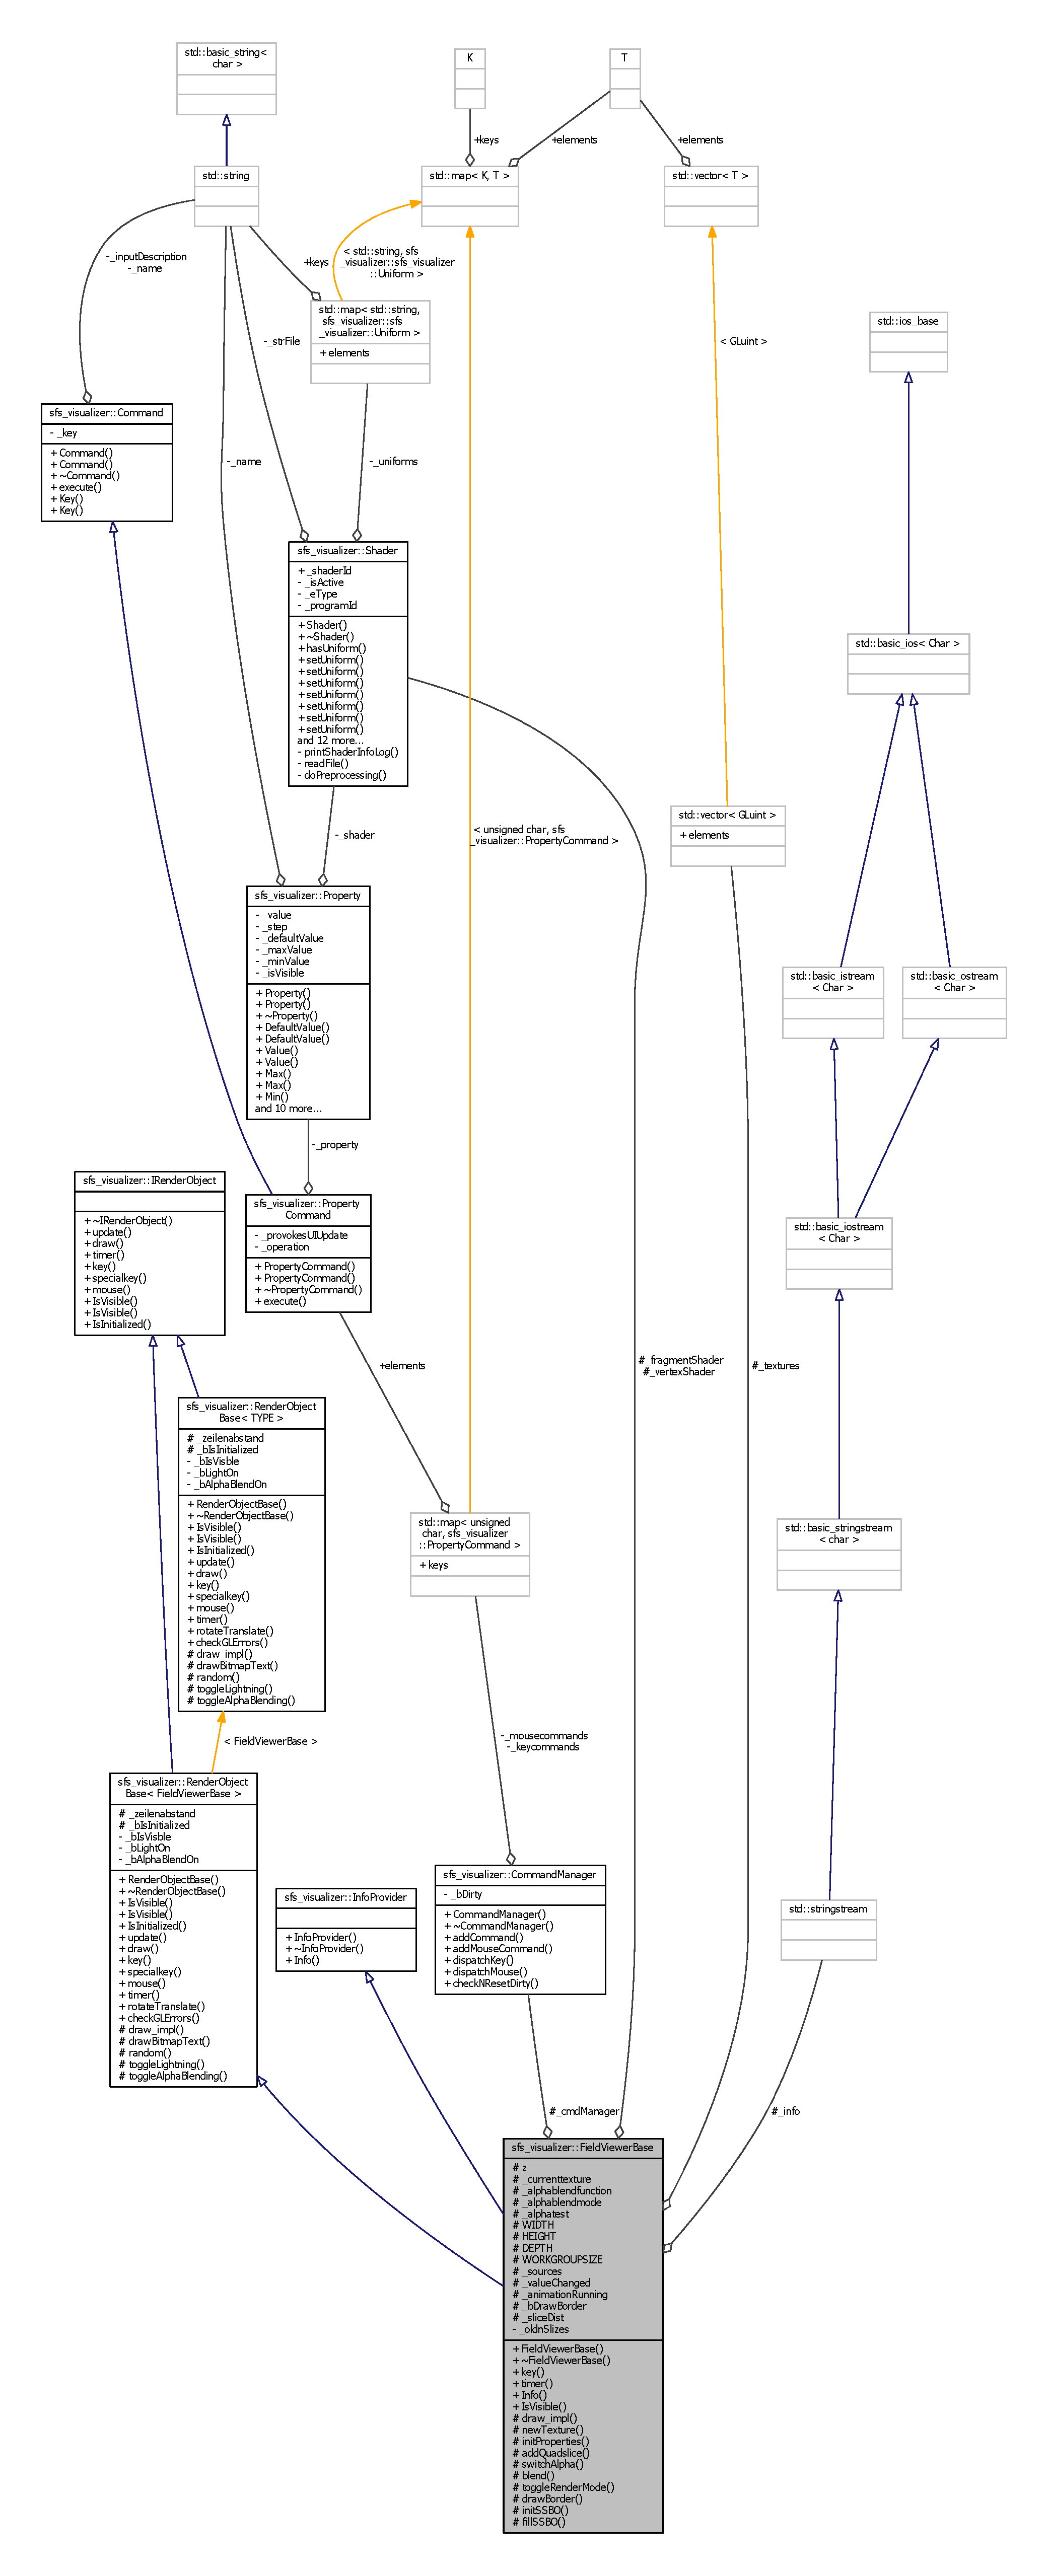
\includegraphics[height=550pt]{da/d20/classsfs__visualizer_1_1FieldViewerBase__coll__graph}
\end{center}
\end{figure}
\subsection*{Public Member Functions}
\begin{DoxyCompactItemize}
\item 
virtual void {\bf key} (unsigned char key, int x, int y)
\begin{DoxyCompactList}\small\item\em user inputs \end{DoxyCompactList}\item 
virtual void {\bfseries timer} (int update\-Rate\-Ms)\label{classsfs__visualizer_1_1FieldViewerBase_afce2b0e2c59465242dbe99ab1721929f}

\item 
virtual const std\-::string {\bf Info} () const 
\begin{DoxyCompactList}\small\item\em Informators and Mutators. \end{DoxyCompactList}\item 
virtual void {\bfseries Is\-Visible} (bool b\-Visible)\label{classsfs__visualizer_1_1FieldViewerBase_a2f44278b92ab84d88cd87ab9395ca6f4}

\end{DoxyCompactItemize}
\subsection*{Protected Member Functions}
\begin{DoxyCompactItemize}
\item 
virtual void {\bfseries draw\-\_\-impl} ()\label{classsfs__visualizer_1_1FieldViewerBase_a4ef48872fe12d12fbcdeac7a9747fc74}

\item 
virtual void {\bfseries new\-Texture} ({\bf Texture\-Factory\-::\-T\-Y\-P\-E} type=Texture\-Factory\-::\-F\-L\-O\-A\-T)\label{classsfs__visualizer_1_1FieldViewerBase_a6039c99ebb2acd34b9fb851c8ba9f0c7}

\item 
virtual void {\bfseries init\-Properties} ()\label{classsfs__visualizer_1_1FieldViewerBase_af1b99b1be47b361a345a7eb459a1514b}

\item 
void {\bfseries add\-Quadslice} (float z\-Offset)\label{classsfs__visualizer_1_1FieldViewerBase_a753cbacdb9eb87bb98ef6ed739014e52}

\item 
void {\bfseries switch\-Alpha} ()\label{classsfs__visualizer_1_1FieldViewerBase_aeb77946af0e21b3fa45c97aae958d101}

\item 
void {\bfseries blend} (int blend)\label{classsfs__visualizer_1_1FieldViewerBase_a618b3410d80b90a5016079ebe8dc2a0f}

\item 
void {\bf toggle\-Render\-Mode} ()
\begin{DoxyCompactList}\small\item\em Toggle between Raytracer and Shearwarping. \end{DoxyCompactList}\item 
void {\bfseries draw\-Border} ()\label{classsfs__visualizer_1_1FieldViewerBase_ad6123cd8caa55d193981aeae657255c1}

\item 
void {\bf init\-S\-S\-B\-O} (G\-Luint index, bool b\-Rand)
\begin{DoxyCompactList}\small\item\em Initializes and creates a \doxyref{Shader}{p.}{dc/dc9/classsfs__visualizer_1_1Shader} Storage Buffer. \end{DoxyCompactList}\item 
void {\bf fill\-S\-S\-B\-O} (const G\-Lvoid $\ast$buffer, G\-Lsizeiptr size, G\-Luint index)
\begin{DoxyCompactList}\small\item\em fill a \doxyref{Shader}{p.}{dc/dc9/classsfs__visualizer_1_1Shader} Storage Buffer with data \end{DoxyCompactList}\end{DoxyCompactItemize}
\subsection*{Protected Attributes}
\begin{DoxyCompactItemize}
\item 
std\-::stringstream {\bfseries \-\_\-info}\label{classsfs__visualizer_1_1FieldViewerBase_a4600455b2a82b08c5caea3769b2a0298}

\item 
std\-::vector$<$ G\-Luint $>$ {\bfseries \-\_\-textures}\label{classsfs__visualizer_1_1FieldViewerBase_a79b08599c03716076725f4b5c0fe9c36}

\item 
float {\bfseries z}\label{classsfs__visualizer_1_1FieldViewerBase_a0b8f59b921c253a61be67137d767c323}

\item 
{\bf Shader} $\ast$ {\bfseries \-\_\-fragment\-Shader}\label{classsfs__visualizer_1_1FieldViewerBase_a4ac4a77b02e50aaf774d733f8dc963a8}

\item 
{\bf Shader} $\ast$ {\bfseries \-\_\-vertex\-Shader}\label{classsfs__visualizer_1_1FieldViewerBase_aef982a3a627dc70874791ed703c59da3}

\item 
int {\bfseries \-\_\-currenttexture}\label{classsfs__visualizer_1_1FieldViewerBase_a7dc92b7ee051cbd936c2bc7334d8167c}

\item 
int {\bfseries \-\_\-alphablendfunction}\label{classsfs__visualizer_1_1FieldViewerBase_a15a0c4adce9bb0cbe2ebaf6619e323c1}

\item 
int {\bfseries \-\_\-alphablendmode}\label{classsfs__visualizer_1_1FieldViewerBase_a998c9d4813ff0dd94b6ef7c571a8501a}

\item 
float {\bfseries \-\_\-alphatest}\label{classsfs__visualizer_1_1FieldViewerBase_a8091b4762cb56e51b432c7d20ed7e098}

\item 
int {\bfseries W\-I\-D\-T\-H}\label{classsfs__visualizer_1_1FieldViewerBase_aa25d9c63660950b1f18d51c13aafabf8}

\item 
int {\bfseries H\-E\-I\-G\-H\-T}\label{classsfs__visualizer_1_1FieldViewerBase_a40969522b0b9d18d6dea9c4dcc3f609d}

\item 
int {\bfseries D\-E\-P\-T\-H}\label{classsfs__visualizer_1_1FieldViewerBase_a6528d82a034a131a899bc86a1ae71539}

\item 
int {\bfseries W\-O\-R\-K\-G\-R\-O\-U\-P\-S\-I\-Z\-E}\label{classsfs__visualizer_1_1FieldViewerBase_a5523768fe7e5371874454009fcfc6eee}

\item 
unsigned int {\bfseries \-\_\-sources}\label{classsfs__visualizer_1_1FieldViewerBase_a12f60e048c8e8373e2a6e68b78c986ae}

\item 
bool {\bfseries \-\_\-value\-Changed}\label{classsfs__visualizer_1_1FieldViewerBase_a459fa2e3e797179596c446e239ed3d8b}

\item 
int {\bfseries \-\_\-animation\-Running}\label{classsfs__visualizer_1_1FieldViewerBase_ab6aa414a798e106478cd1e08fe2d9398}

\item 
bool {\bfseries \-\_\-b\-Draw\-Border}\label{classsfs__visualizer_1_1FieldViewerBase_a4e29f6e3892ef790d6e018555bb0dc89}

\item 
{\bf Command\-Manager} {\bfseries \-\_\-cmd\-Manager}\label{classsfs__visualizer_1_1FieldViewerBase_a1077fecc40938937ab1c34146a545754}

\item 
float {\bfseries \-\_\-slice\-Dist}\label{classsfs__visualizer_1_1FieldViewerBase_a536f6a3e90ca80f55a0081ad026e62b2}

\end{DoxyCompactItemize}
\subsection*{Private Attributes}
\begin{DoxyCompactItemize}
\item 
int {\bfseries \-\_\-oldn\-Slizes}\label{classsfs__visualizer_1_1FieldViewerBase_aadbce9bdcaa48cf8ac0b5c512ac018f5}

\end{DoxyCompactItemize}
\subsection*{Additional Inherited Members}


\subsection{Detailed Description}
A Base class for classes that can show soundfields either with shearwarping or a raytracer. 

Definition at line 35 of file fieldviewerbase.\-h.



\subsection{Member Function Documentation}
\index{sfs\-\_\-visualizer\-::\-Field\-Viewer\-Base@{sfs\-\_\-visualizer\-::\-Field\-Viewer\-Base}!key@{key}}
\index{key@{key}!sfs_visualizer::FieldViewerBase@{sfs\-\_\-visualizer\-::\-Field\-Viewer\-Base}}
\subsubsection[{key}]{\setlength{\rightskip}{0pt plus 5cm}void Field\-Viewer\-Base\-::key (
\begin{DoxyParamCaption}
\item[{unsigned char}]{key, }
\item[{int}]{x, }
\item[{int}]{y}
\end{DoxyParamCaption}
)\hspace{0.3cm}{\ttfamily [virtual]}}\label{classsfs__visualizer_1_1FieldViewerBase_acebb098dc25cd342be007c47cc2e64ab}


user inputs 



Reimplemented from {\bf sfs\-\_\-visualizer\-::\-Render\-Object\-Base$<$ Field\-Viewer\-Base $>$} \doxyref{}{p.}{de/d2a/classsfs__visualizer_1_1RenderObjectBase_a3f0106a0ce3861f34e5330da65e7bdd4}.



Reimplemented in {\bf sfs\-\_\-visualizer\-::\-Shader\-Soundfield\-Viewer\-Green} \doxyref{}{p.}{d6/dab/classsfs__visualizer_1_1ShaderSoundfieldViewerGreen_a5a2363722318f189a5c5276d64659776}, and {\bf sfs\-\_\-visualizer\-::\-Matlab\-Field\-Viewer} \doxyref{}{p.}{d8/d1c/classsfs__visualizer_1_1MatlabFieldViewer_aaba2a2a82434165851e44a01f299d58b}.



Definition at line 212 of file fieldviewerbase.\-cpp.



References toggle\-Render\-Mode().



Referenced by sfs\-\_\-visualizer\-::\-Matlab\-Field\-Viewer\-::key().

\index{sfs\-\_\-visualizer\-::\-Field\-Viewer\-Base@{sfs\-\_\-visualizer\-::\-Field\-Viewer\-Base}!Info@{Info}}
\index{Info@{Info}!sfs_visualizer::FieldViewerBase@{sfs\-\_\-visualizer\-::\-Field\-Viewer\-Base}}
\subsubsection[{Info}]{\setlength{\rightskip}{0pt plus 5cm}const std\-::string Field\-Viewer\-Base\-::\-Info (
\begin{DoxyParamCaption}
{}
\end{DoxyParamCaption}
) const\hspace{0.3cm}{\ttfamily [virtual]}}\label{classsfs__visualizer_1_1FieldViewerBase_af63499897a2d254892ff1d4f1506c672}


Informators and Mutators. 



Implements {\bf sfs\-\_\-visualizer\-::\-Info\-Provider} \doxyref{}{p.}{d4/dd0/classsfs__visualizer_1_1InfoProvider_a654fcc238d83d144ecbb1becadd87f76}.



Definition at line 441 of file fieldviewerbase.\-cpp.

\index{sfs\-\_\-visualizer\-::\-Field\-Viewer\-Base@{sfs\-\_\-visualizer\-::\-Field\-Viewer\-Base}!toggle\-Render\-Mode@{toggle\-Render\-Mode}}
\index{toggle\-Render\-Mode@{toggle\-Render\-Mode}!sfs_visualizer::FieldViewerBase@{sfs\-\_\-visualizer\-::\-Field\-Viewer\-Base}}
\subsubsection[{toggle\-Render\-Mode}]{\setlength{\rightskip}{0pt plus 5cm}void Field\-Viewer\-Base\-::toggle\-Render\-Mode (
\begin{DoxyParamCaption}
{}
\end{DoxyParamCaption}
)\hspace{0.3cm}{\ttfamily [protected]}}\label{classsfs__visualizer_1_1FieldViewerBase_a5824457af85b00f657ded7cebf062d80}


Toggle between Raytracer and Shearwarping. 



Definition at line 173 of file fieldviewerbase.\-cpp.



Referenced by key().

\index{sfs\-\_\-visualizer\-::\-Field\-Viewer\-Base@{sfs\-\_\-visualizer\-::\-Field\-Viewer\-Base}!init\-S\-S\-B\-O@{init\-S\-S\-B\-O}}
\index{init\-S\-S\-B\-O@{init\-S\-S\-B\-O}!sfs_visualizer::FieldViewerBase@{sfs\-\_\-visualizer\-::\-Field\-Viewer\-Base}}
\subsubsection[{init\-S\-S\-B\-O}]{\setlength{\rightskip}{0pt plus 5cm}void Field\-Viewer\-Base\-::init\-S\-S\-B\-O (
\begin{DoxyParamCaption}
\item[{G\-Luint}]{index, }
\item[{bool}]{b\-Rand = {\ttfamily false}}
\end{DoxyParamCaption}
)\hspace{0.3cm}{\ttfamily [protected]}}\label{classsfs__visualizer_1_1FieldViewerBase_ad19f73d7baa1edea505a9809f14fea56}


Initializes and creates a \doxyref{Shader}{p.}{dc/dc9/classsfs__visualizer_1_1Shader} Storage Buffer. 



Definition at line 157 of file fieldviewerbase.\-cpp.



References fill\-S\-S\-B\-O(), and sfs\-\_\-visualizer\-::\-Render\-Object\-Base$<$ Field\-Viewer\-Base $>$\-::random().

\index{sfs\-\_\-visualizer\-::\-Field\-Viewer\-Base@{sfs\-\_\-visualizer\-::\-Field\-Viewer\-Base}!fill\-S\-S\-B\-O@{fill\-S\-S\-B\-O}}
\index{fill\-S\-S\-B\-O@{fill\-S\-S\-B\-O}!sfs_visualizer::FieldViewerBase@{sfs\-\_\-visualizer\-::\-Field\-Viewer\-Base}}
\subsubsection[{fill\-S\-S\-B\-O}]{\setlength{\rightskip}{0pt plus 5cm}void Field\-Viewer\-Base\-::fill\-S\-S\-B\-O (
\begin{DoxyParamCaption}
\item[{const G\-Lvoid $\ast$}]{buffer, }
\item[{G\-Lsizeiptr}]{size, }
\item[{G\-Luint}]{index}
\end{DoxyParamCaption}
)\hspace{0.3cm}{\ttfamily [protected]}}\label{classsfs__visualizer_1_1FieldViewerBase_abdad8b23a40d70397949efbc45609a47}


fill a \doxyref{Shader}{p.}{dc/dc9/classsfs__visualizer_1_1Shader} Storage Buffer with data 



Definition at line 133 of file fieldviewerbase.\-cpp.



Referenced by init\-S\-S\-B\-O().



The documentation for this class was generated from the following files\-:\begin{DoxyCompactItemize}
\item 
fieldviewerbase.\-h\item 
fieldviewerbase.\-cpp\end{DoxyCompactItemize}

\section{sfs\-\_\-visualizer\-:\-:Help\-Overlay Class Reference}
\label{classsfs__visualizer_1_1HelpOverlay}\index{sfs\-\_\-visualizer\-::\-Help\-Overlay@{sfs\-\_\-visualizer\-::\-Help\-Overlay}}


A Render\-Object, that displays the help menu.  




{\ttfamily \#include $<$helpoverlay.\-h$>$}



Inheritance diagram for sfs\-\_\-visualizer\-:\-:Help\-Overlay\-:\nopagebreak
\begin{figure}[H]
\begin{center}
\leavevmode
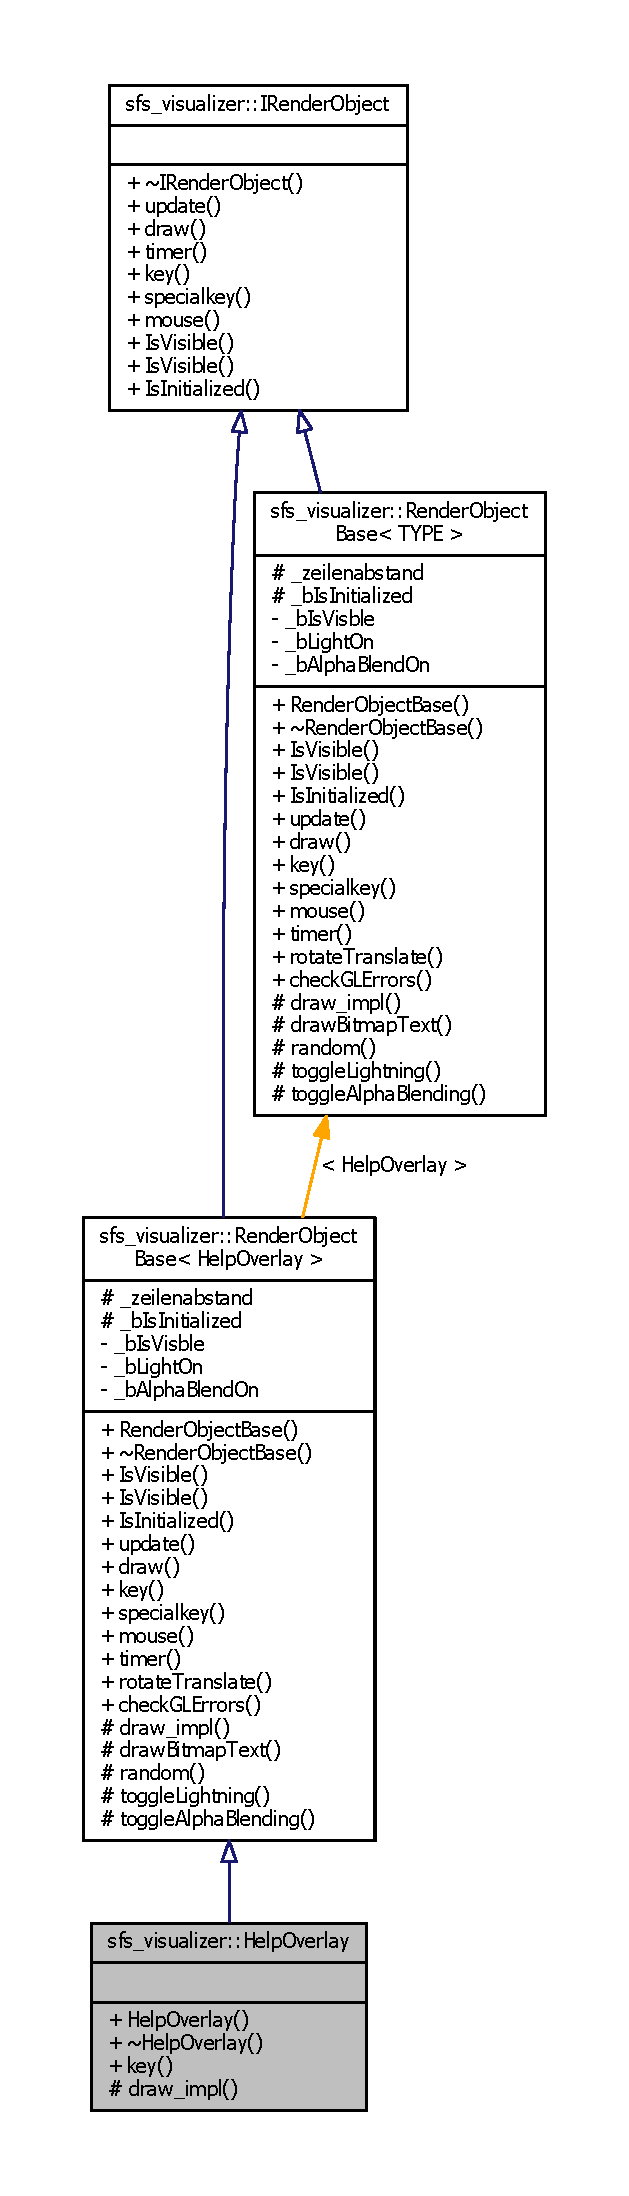
\includegraphics[height=550pt]{d4/d09/classsfs__visualizer_1_1HelpOverlay__inherit__graph}
\end{center}
\end{figure}


Collaboration diagram for sfs\-\_\-visualizer\-:\-:Help\-Overlay\-:\nopagebreak
\begin{figure}[H]
\begin{center}
\leavevmode
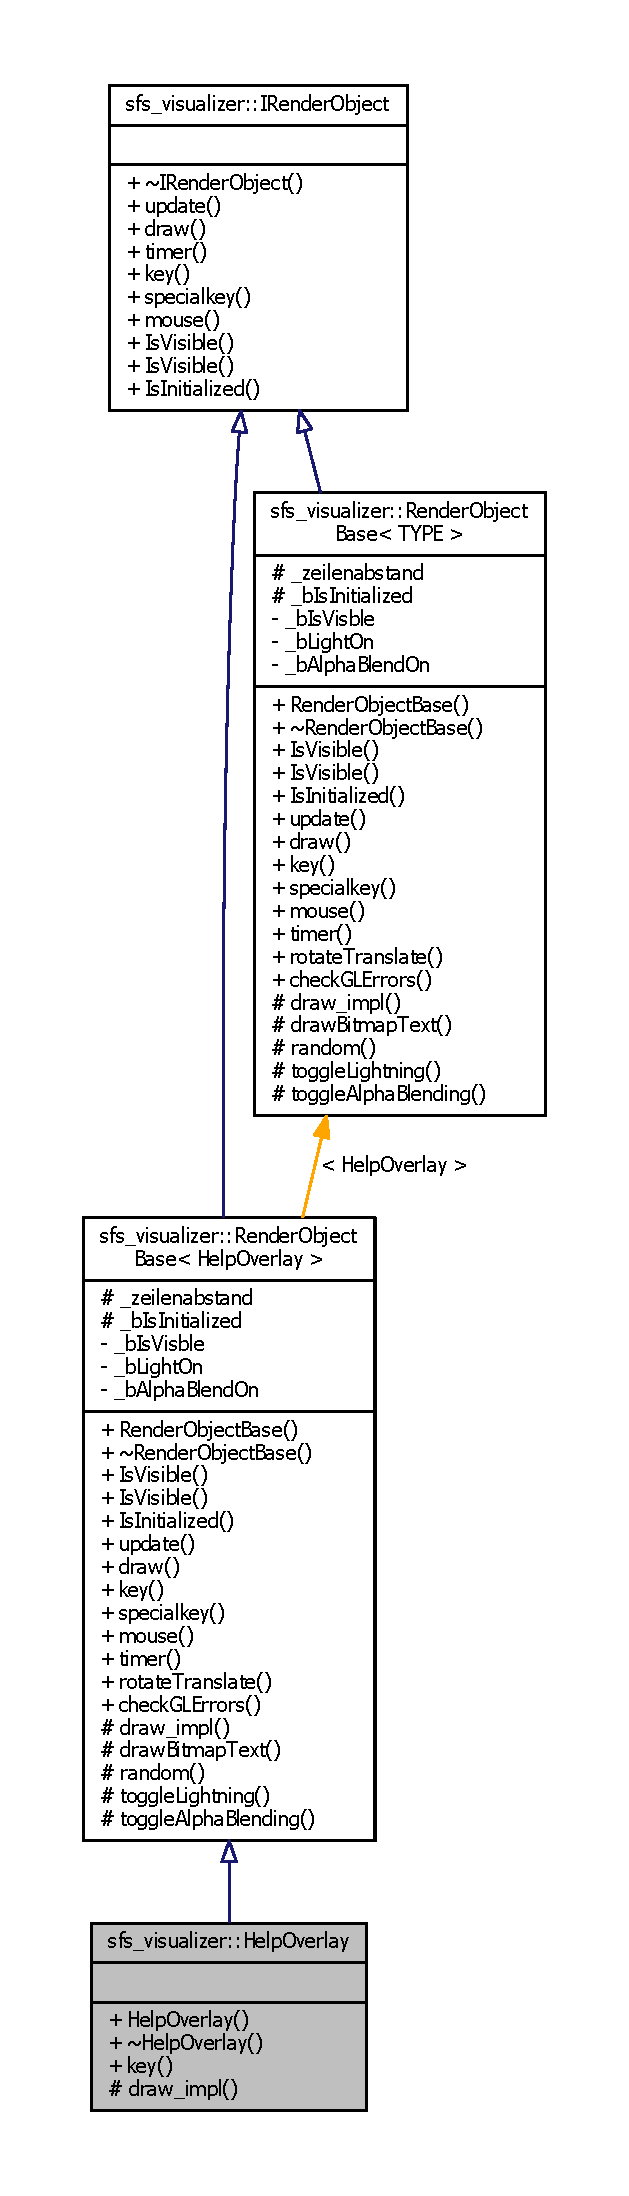
\includegraphics[height=550pt]{d5/d22/classsfs__visualizer_1_1HelpOverlay__coll__graph}
\end{center}
\end{figure}
\subsection*{Public Member Functions}
\begin{DoxyCompactItemize}
\item 
virtual void {\bf key} (unsigned char key, int x, int y)
\begin{DoxyCompactList}\small\item\em user inputs \end{DoxyCompactList}\end{DoxyCompactItemize}
\subsection*{Protected Member Functions}
\begin{DoxyCompactItemize}
\item 
virtual void {\bfseries draw\-\_\-impl} ()\label{classsfs__visualizer_1_1HelpOverlay_afb3970155bd20bb94ee9dae0ea2958d5}

\end{DoxyCompactItemize}
\subsection*{Additional Inherited Members}


\subsection{Detailed Description}
A Render\-Object, that displays the help menu. 

Definition at line 24 of file helpoverlay.\-h.



\subsection{Member Function Documentation}
\index{sfs\-\_\-visualizer\-::\-Help\-Overlay@{sfs\-\_\-visualizer\-::\-Help\-Overlay}!key@{key}}
\index{key@{key}!sfs_visualizer::HelpOverlay@{sfs\-\_\-visualizer\-::\-Help\-Overlay}}
\subsubsection[{key}]{\setlength{\rightskip}{0pt plus 5cm}void Help\-Overlay\-::key (
\begin{DoxyParamCaption}
\item[{unsigned char}]{key, }
\item[{int}]{x, }
\item[{int}]{y}
\end{DoxyParamCaption}
)\hspace{0.3cm}{\ttfamily [virtual]}}\label{classsfs__visualizer_1_1HelpOverlay_af073d80d01dc30a14a40238b9d539d14}


user inputs 



Reimplemented from {\bf sfs\-\_\-visualizer\-::\-Render\-Object\-Base$<$ Help\-Overlay $>$} \doxyref{}{p.}{de/d2a/classsfs__visualizer_1_1RenderObjectBase_a3f0106a0ce3861f34e5330da65e7bdd4}.



Definition at line 18 of file helpoverlay.\-cpp.



References sfs\-\_\-visualizer\-::\-Render\-Object\-Base$<$ Help\-Overlay $>$\-::\-Is\-Visible().



The documentation for this class was generated from the following files\-:\begin{DoxyCompactItemize}
\item 
helpoverlay.\-h\item 
helpoverlay.\-cpp\end{DoxyCompactItemize}

\section{Help\-Overlay Class Reference}
\label{classHelpOverlay}\index{Help\-Overlay@{Help\-Overlay}}


{\ttfamily \#include $<$helpoverlay.\-h$>$}



Collaboration diagram for Help\-Overlay\-:
\nopagebreak
\begin{figure}[H]
\begin{center}
\leavevmode
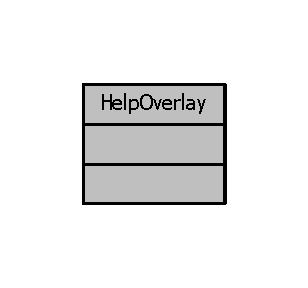
\includegraphics[width=148pt]{d8/dc5/classHelpOverlay__coll__graph}
\end{center}
\end{figure}


\subsection{Detailed Description}
\begin{DoxyAuthor}{Author}
Marcus Zepp
\end{DoxyAuthor}
\begin{DoxyVersion}{Version}

\end{DoxyVersion}
\begin{DoxyParagraph}{Revision\-:}
1.\-0 
\end{DoxyParagraph}


\begin{DoxyDate}{Date}

\end{DoxyDate}
\begin{DoxyParagraph}{Date\-:}
2014/03/26 14\-:16\-:20 
\end{DoxyParagraph}


Contact\-: {\tt zeppfisj@mailbox.\-tu-\/berlin.\-de} 

The documentation for this class was generated from the following file\-:\begin{DoxyCompactItemize}
\item 
helpoverlay.\-h\end{DoxyCompactItemize}

\section{Info\-Overlay Class Reference}
\label{classInfoOverlay}\index{Info\-Overlay@{Info\-Overlay}}


{\ttfamily \#include $<$infooverlay.\-h$>$}



Collaboration diagram for Info\-Overlay\-:\nopagebreak
\begin{figure}[H]
\begin{center}
\leavevmode
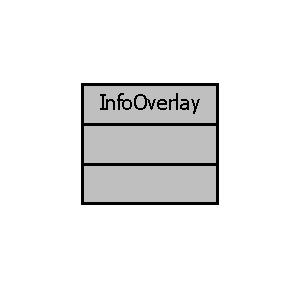
\includegraphics[width=144pt]{da/d7f/classInfoOverlay__coll__graph}
\end{center}
\end{figure}


\subsection{Detailed Description}
\begin{DoxyAuthor}{Author}
Marcus Zepp
\end{DoxyAuthor}
\begin{DoxyVersion}{Version}

\end{DoxyVersion}
\begin{DoxyParagraph}{Revision\-:}
1.\-0 
\end{DoxyParagraph}


\begin{DoxyDate}{Date}

\end{DoxyDate}
\begin{DoxyParagraph}{Date\-:}
2014/03/26 14\-:16\-:20 
\end{DoxyParagraph}


Contact\-: {\tt zeppfisj@mailbox.\-tu-\/berlin.\-de} 

The documentation for this class was generated from the following file\-:\begin{DoxyCompactItemize}
\item 
infooverlay.\-h\end{DoxyCompactItemize}

\section{sfs\-\_\-visualizer\-:\-:Info\-Overlay Class Reference}
\label{classsfs__visualizer_1_1InfoOverlay}\index{sfs\-\_\-visualizer\-::\-Info\-Overlay@{sfs\-\_\-visualizer\-::\-Info\-Overlay}}


A Render\-Object, that displays the information overlay.  




{\ttfamily \#include $<$infooverlay.\-h$>$}



Inheritance diagram for sfs\-\_\-visualizer\-:\-:Info\-Overlay\-:\nopagebreak
\begin{figure}[H]
\begin{center}
\leavevmode
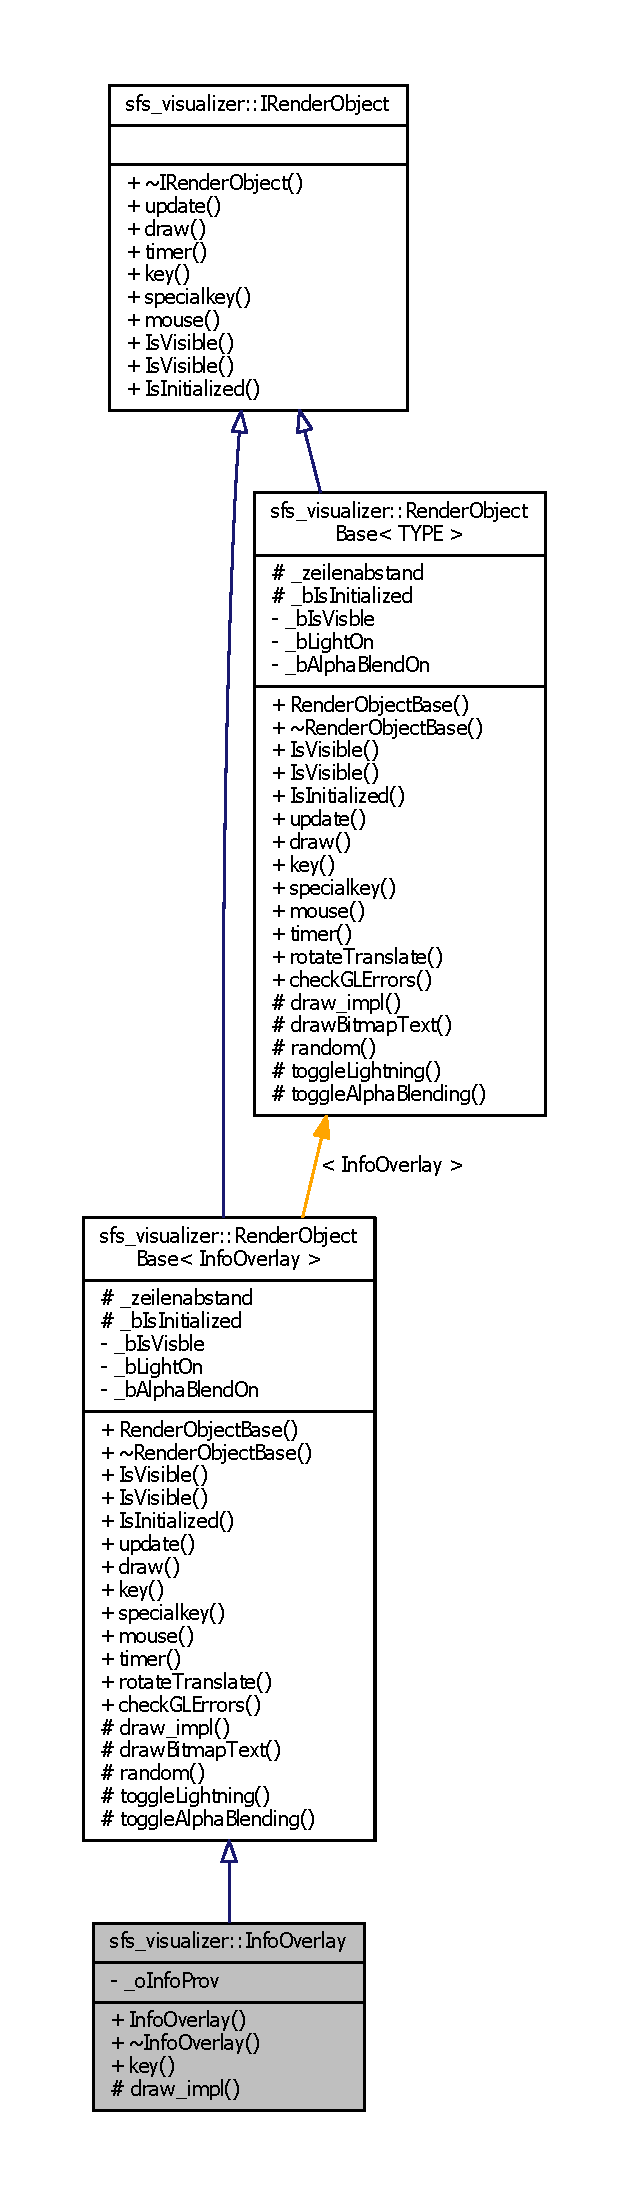
\includegraphics[height=550pt]{de/d22/classsfs__visualizer_1_1InfoOverlay__inherit__graph}
\end{center}
\end{figure}


Collaboration diagram for sfs\-\_\-visualizer\-:\-:Info\-Overlay\-:\nopagebreak
\begin{figure}[H]
\begin{center}
\leavevmode
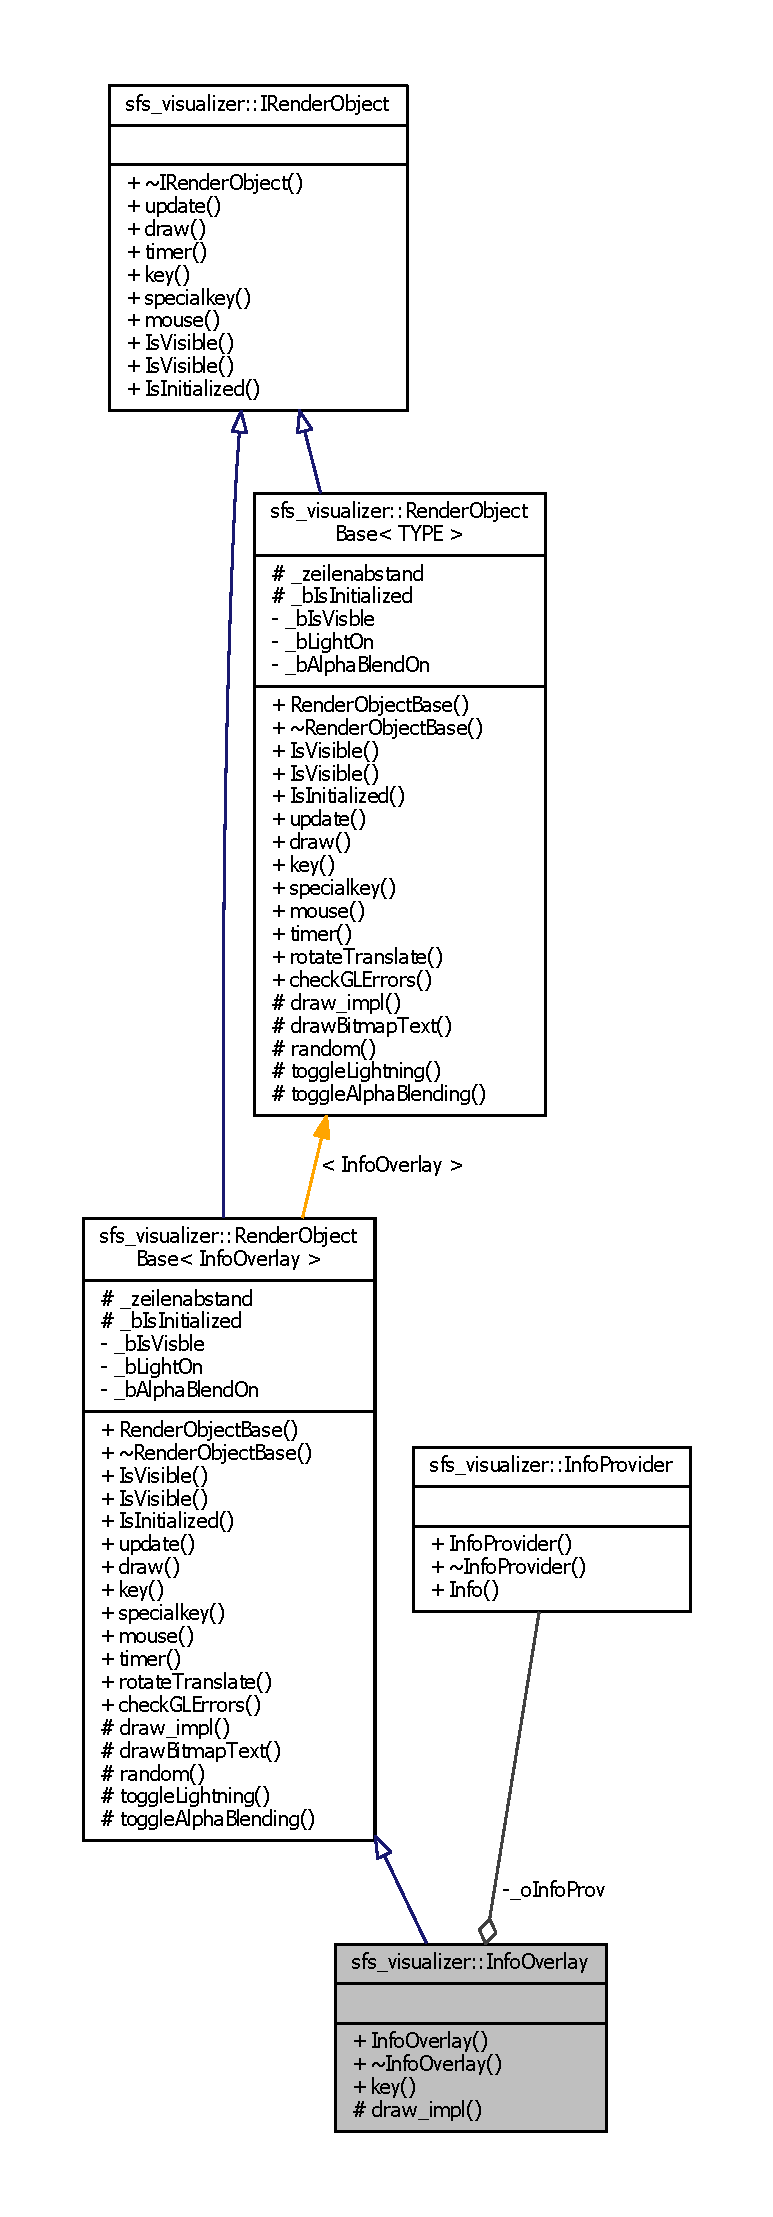
\includegraphics[height=550pt]{d1/d65/classsfs__visualizer_1_1InfoOverlay__coll__graph}
\end{center}
\end{figure}
\subsection*{Public Member Functions}
\begin{DoxyCompactItemize}
\item 
{\bfseries Info\-Overlay} ({\bf Info\-Provider} \&info\-Prov)\label{classsfs__visualizer_1_1InfoOverlay_a879c32293f4a96eb0adcb85ef975be8f}

\item 
virtual void {\bf key} (unsigned char key, int x, int y)
\begin{DoxyCompactList}\small\item\em user inputs \end{DoxyCompactList}\end{DoxyCompactItemize}
\subsection*{Protected Member Functions}
\begin{DoxyCompactItemize}
\item 
virtual void {\bfseries draw\-\_\-impl} ()\label{classsfs__visualizer_1_1InfoOverlay_a8b17bd3b9caa90af105e0bf6c6498653}

\end{DoxyCompactItemize}
\subsection*{Private Attributes}
\begin{DoxyCompactItemize}
\item 
{\bf Info\-Provider} \& {\bfseries \-\_\-o\-Info\-Prov}\label{classsfs__visualizer_1_1InfoOverlay_a38fa1f8ec11a866cada16aa9d61f1e3d}

\end{DoxyCompactItemize}
\subsection*{Additional Inherited Members}


\subsection{Detailed Description}
A Render\-Object, that displays the information overlay. 

Definition at line 25 of file infooverlay.\-h.



\subsection{Member Function Documentation}
\index{sfs\-\_\-visualizer\-::\-Info\-Overlay@{sfs\-\_\-visualizer\-::\-Info\-Overlay}!key@{key}}
\index{key@{key}!sfs_visualizer::InfoOverlay@{sfs\-\_\-visualizer\-::\-Info\-Overlay}}
\subsubsection[{key}]{\setlength{\rightskip}{0pt plus 5cm}void Info\-Overlay\-::key (
\begin{DoxyParamCaption}
\item[{unsigned char}]{key, }
\item[{int}]{x, }
\item[{int}]{y}
\end{DoxyParamCaption}
)\hspace{0.3cm}{\ttfamily [virtual]}}\label{classsfs__visualizer_1_1InfoOverlay_ad04dcece97043b948ae9af471172e5c0}


user inputs 



Reimplemented from {\bf sfs\-\_\-visualizer\-::\-Render\-Object\-Base$<$ Info\-Overlay $>$} \doxyref{}{p.}{de/d2a/classsfs__visualizer_1_1RenderObjectBase_a3f0106a0ce3861f34e5330da65e7bdd4}.



Definition at line 15 of file infooverlay.\-cpp.



References sfs\-\_\-visualizer\-::\-Render\-Object\-Base$<$ Info\-Overlay $>$\-::\-Is\-Visible().



The documentation for this class was generated from the following files\-:\begin{DoxyCompactItemize}
\item 
infooverlay.\-h\item 
infooverlay.\-cpp\end{DoxyCompactItemize}

\section{sfs\-\_\-visualizer\-:\-:Info\-Provider Class Reference}
\label{classsfs__visualizer_1_1InfoProvider}\index{sfs\-\_\-visualizer\-::\-Info\-Provider@{sfs\-\_\-visualizer\-::\-Info\-Provider}}


Interface for objects, that want infos to be displayed in the \doxyref{Info\-Overlay}{p.}{d7/d78/classsfs__visualizer_1_1InfoOverlay}.  




{\ttfamily \#include $<$infoprovider.\-h$>$}



Inheritance diagram for sfs\-\_\-visualizer\-:\-:Info\-Provider\-:
\nopagebreak
\begin{figure}[H]
\begin{center}
\leavevmode
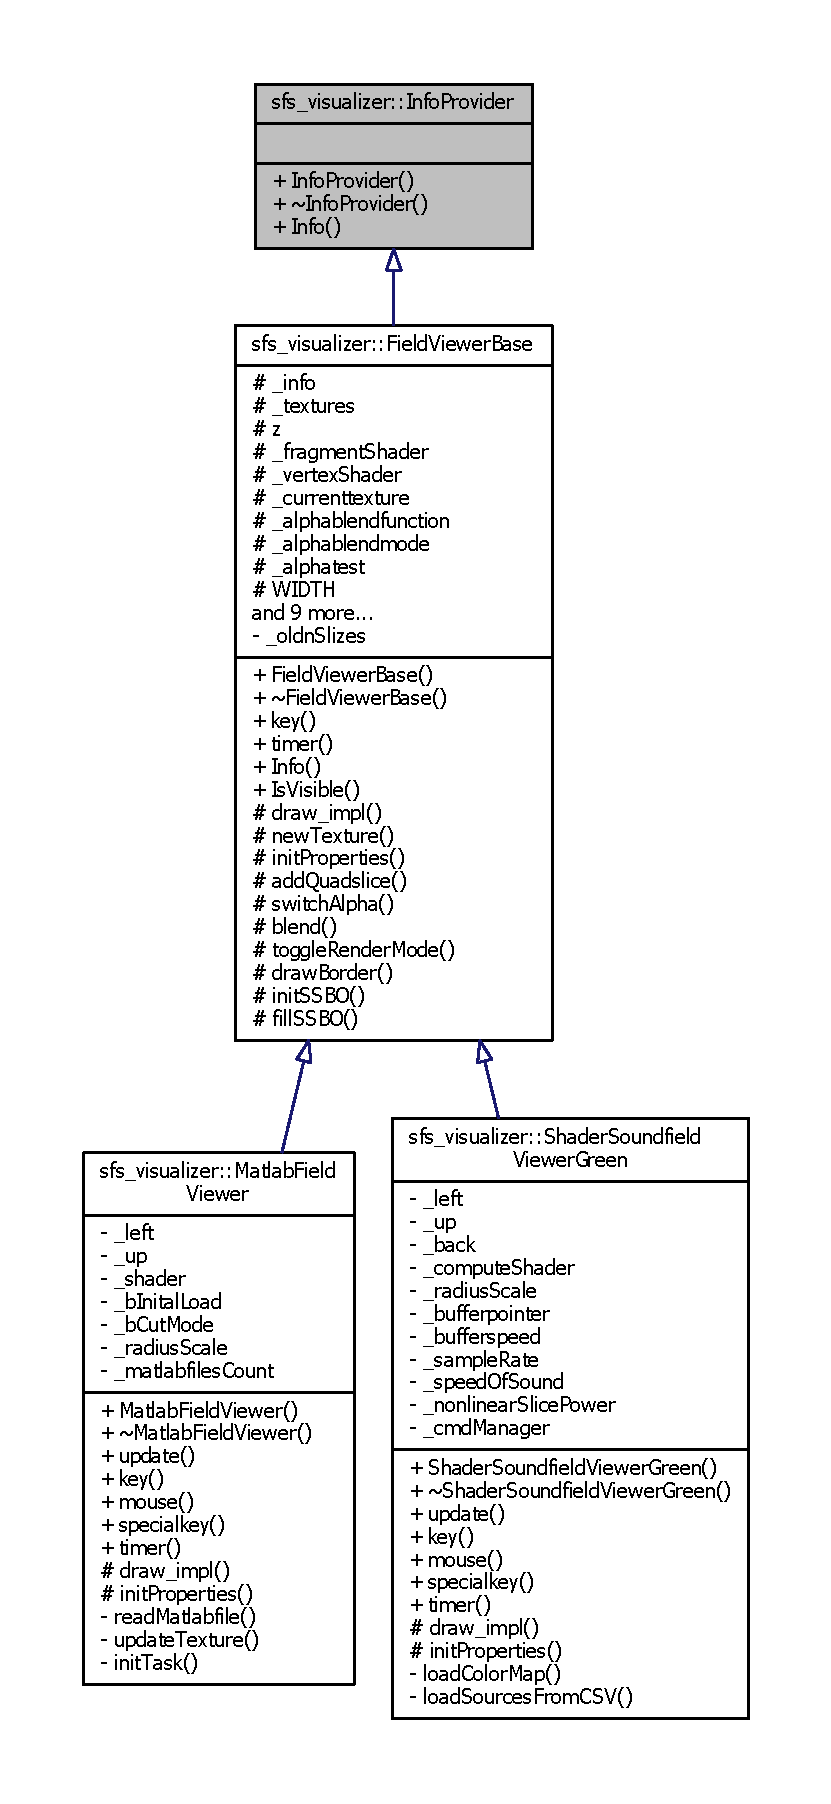
\includegraphics[height=550pt]{d4/daa/classsfs__visualizer_1_1InfoProvider__inherit__graph}
\end{center}
\end{figure}


Collaboration diagram for sfs\-\_\-visualizer\-:\-:Info\-Provider\-:\nopagebreak
\begin{figure}[H]
\begin{center}
\leavevmode
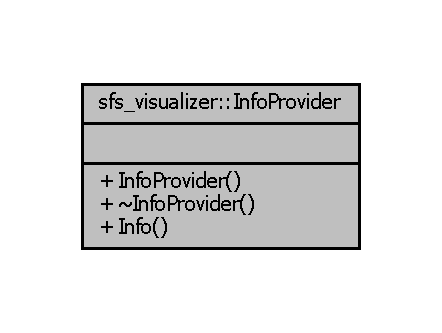
\includegraphics[width=212pt]{d6/de5/classsfs__visualizer_1_1InfoProvider__coll__graph}
\end{center}
\end{figure}
\subsection*{Public Member Functions}
\begin{DoxyCompactItemize}
\item 
virtual const std\-::string {\bf Info} () const =0
\begin{DoxyCompactList}\small\item\em Informators. \end{DoxyCompactList}\end{DoxyCompactItemize}


\subsection{Detailed Description}
Interface for objects, that want infos to be displayed in the \doxyref{Info\-Overlay}{p.}{d7/d78/classsfs__visualizer_1_1InfoOverlay}. 

Definition at line 25 of file infoprovider.\-h.



\subsection{Member Function Documentation}
\index{sfs\-\_\-visualizer\-::\-Info\-Provider@{sfs\-\_\-visualizer\-::\-Info\-Provider}!Info@{Info}}
\index{Info@{Info}!sfs_visualizer::InfoProvider@{sfs\-\_\-visualizer\-::\-Info\-Provider}}
\subsubsection[{Info}]{\setlength{\rightskip}{0pt plus 5cm}virtual const std\-::string sfs\-\_\-visualizer\-::\-Info\-Provider\-::\-Info (
\begin{DoxyParamCaption}
{}
\end{DoxyParamCaption}
) const\hspace{0.3cm}{\ttfamily [pure virtual]}}\label{classsfs__visualizer_1_1InfoProvider_a654fcc238d83d144ecbb1becadd87f76}


Informators. 



Implemented in {\bf sfs\-\_\-visualizer\-::\-Field\-Viewer\-Base} \doxyref{}{p.}{dc/dc0/classsfs__visualizer_1_1FieldViewerBase_af63499897a2d254892ff1d4f1506c672}.



The documentation for this class was generated from the following files\-:\begin{DoxyCompactItemize}
\item 
infoprovider.\-h\item 
infoprovider.\-cpp\end{DoxyCompactItemize}

\section{Info\-Provider Class Reference}
\label{classInfoProvider}\index{Info\-Provider@{Info\-Provider}}


{\ttfamily \#include $<$infoprovider.\-h$>$}



Collaboration diagram for Info\-Provider\-:
\nopagebreak
\begin{figure}[H]
\begin{center}
\leavevmode
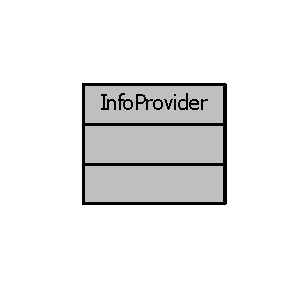
\includegraphics[width=148pt]{d2/dd5/classInfoProvider__coll__graph}
\end{center}
\end{figure}


\subsection{Detailed Description}
\begin{DoxyAuthor}{Author}
Marcus Zepp
\end{DoxyAuthor}
\begin{DoxyVersion}{Version}

\end{DoxyVersion}
\begin{DoxyParagraph}{Revision\-:}
1.\-0 
\end{DoxyParagraph}


\begin{DoxyDate}{Date}

\end{DoxyDate}
\begin{DoxyParagraph}{Date\-:}
2014/03/26 14\-:16\-:20 
\end{DoxyParagraph}


Contact\-: {\tt zeppfisj@mailbox.\-tu-\/berlin.\-de} 

The documentation for this class was generated from the following file\-:\begin{DoxyCompactItemize}
\item 
infoprovider.\-h\end{DoxyCompactItemize}

\section{sfs\-\_\-visualizer\-:\-:I\-Render\-Object Class Reference}
\label{classsfs__visualizer_1_1IRenderObject}\index{sfs\-\_\-visualizer\-::\-I\-Render\-Object@{sfs\-\_\-visualizer\-::\-I\-Render\-Object}}


Interface of all objects, that can be shown by the renderengine.  




{\ttfamily \#include $<$renderobject.\-h$>$}



Inheritance diagram for sfs\-\_\-visualizer\-:\-:I\-Render\-Object\-:
\nopagebreak
\begin{figure}[H]
\begin{center}
\leavevmode
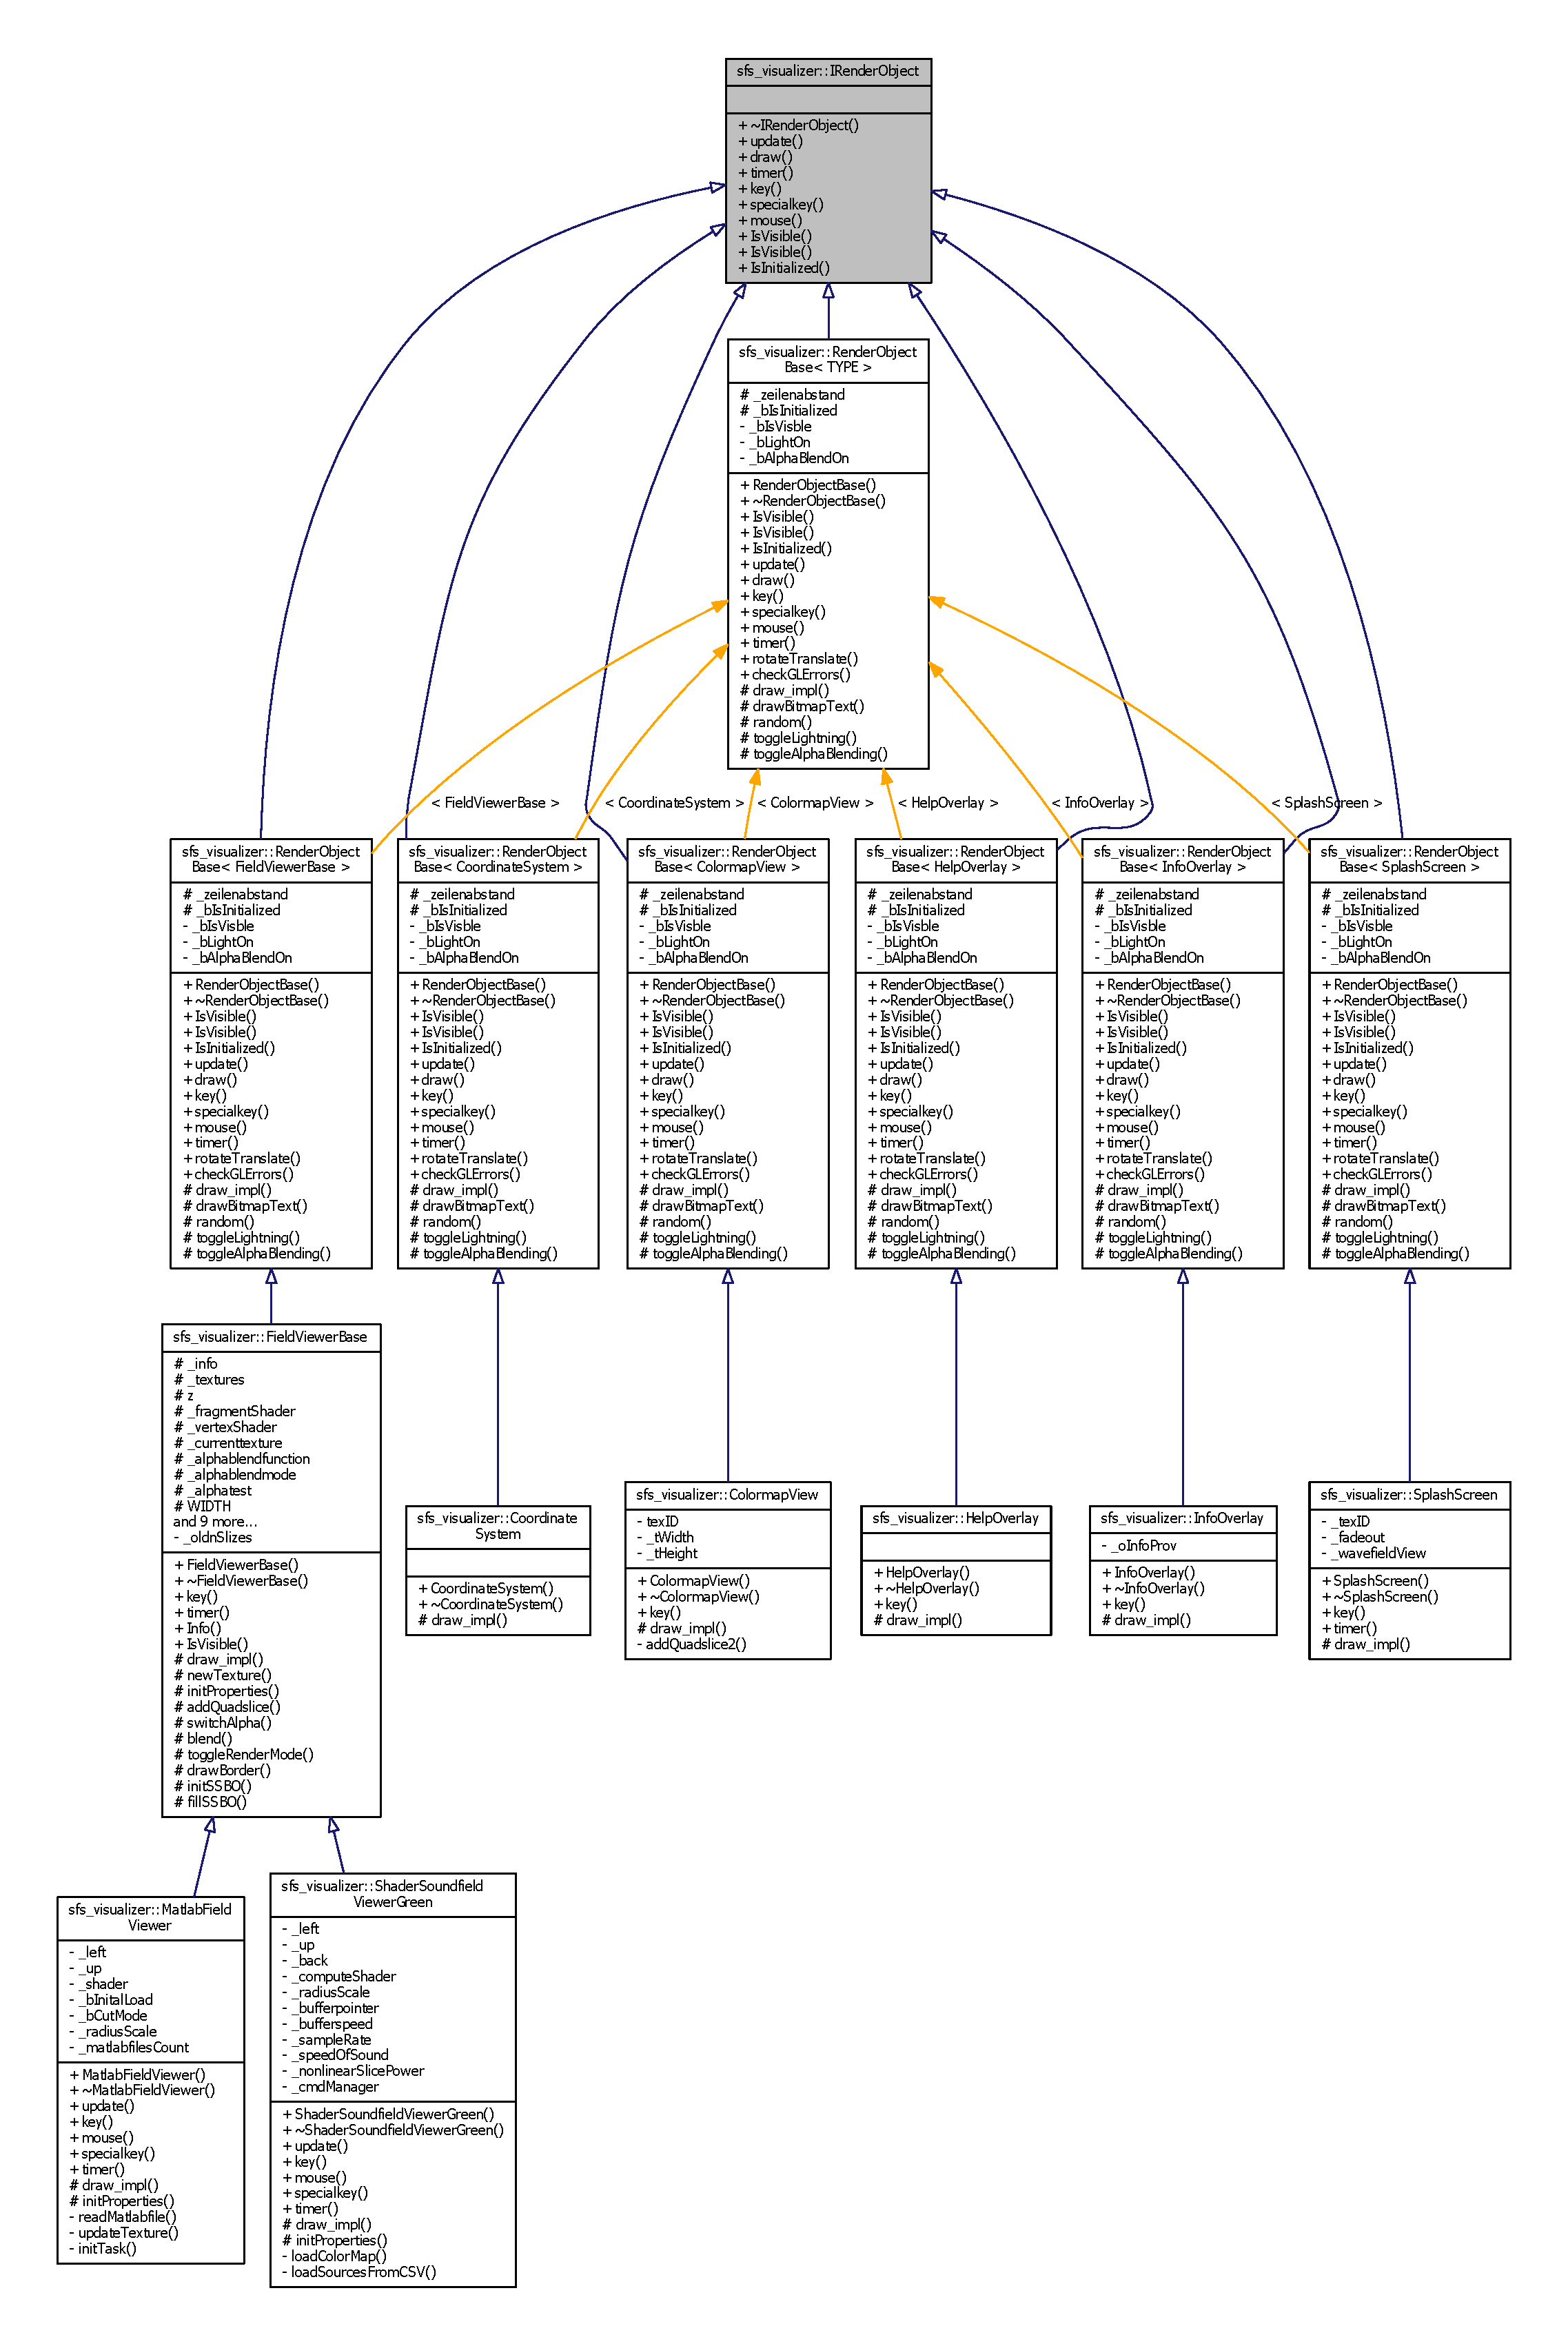
\includegraphics[width=350pt]{d0/dde/classsfs__visualizer_1_1IRenderObject__inherit__graph}
\end{center}
\end{figure}


Collaboration diagram for sfs\-\_\-visualizer\-:\-:I\-Render\-Object\-:\nopagebreak
\begin{figure}[H]
\begin{center}
\leavevmode
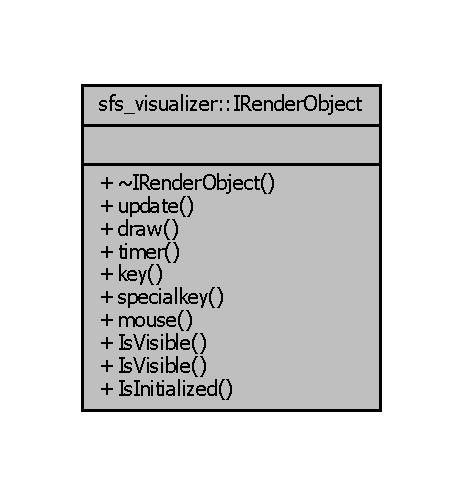
\includegraphics[width=222pt]{df/d49/classsfs__visualizer_1_1IRenderObject__coll__graph}
\end{center}
\end{figure}
\subsection*{Public Member Functions}
\begin{DoxyCompactItemize}
\item 
virtual void {\bf update} ()=0
\begin{DoxyCompactList}\small\item\em methods \end{DoxyCompactList}\item 
virtual void {\bfseries draw} ()=0\label{classsfs__visualizer_1_1IRenderObject_a3dfa50bfffefdaa6b72d912d4120ab71}

\item 
virtual void {\bfseries timer} (int update\-Rate\-Ms)=0\label{classsfs__visualizer_1_1IRenderObject_aae7260514a73933da78dc4d54fbfe81f}

\item 
virtual void {\bf key} (unsigned char key, int x, int y)=0
\begin{DoxyCompactList}\small\item\em user inputs \end{DoxyCompactList}\item 
virtual void {\bfseries specialkey} (int {\bf key}, int x, int y)=0\label{classsfs__visualizer_1_1IRenderObject_aec12d8efed0f18273a68bf3dc6b1f9e5}

\item 
virtual void {\bfseries mouse} (int button, int state, int x, int y)=0\label{classsfs__visualizer_1_1IRenderObject_ad5879f94695eb48af3d5eeca63212809}

\item 
virtual bool {\bf Is\-Visible} ()=0
\begin{DoxyCompactList}\small\item\em mutators and informators \end{DoxyCompactList}\item 
virtual void {\bfseries Is\-Visible} (bool)=0\label{classsfs__visualizer_1_1IRenderObject_a48868419eabd97f0871a2b7b9484c4f3}

\item 
virtual bool {\bfseries Is\-Initialized} ()=0\label{classsfs__visualizer_1_1IRenderObject_ac16bc7487ceb527a4dd7568d3fd6ced0}

\end{DoxyCompactItemize}


\subsection{Detailed Description}
Interface of all objects, that can be shown by the renderengine. 

they handle mouse-\/ and keyevents A timer is called from the renderthread to do regular tasks like recalculations for animations. 

Definition at line 23 of file renderobject.\-h.



\subsection{Member Function Documentation}
\index{sfs\-\_\-visualizer\-::\-I\-Render\-Object@{sfs\-\_\-visualizer\-::\-I\-Render\-Object}!update@{update}}
\index{update@{update}!sfs_visualizer::IRenderObject@{sfs\-\_\-visualizer\-::\-I\-Render\-Object}}
\subsubsection[{update}]{\setlength{\rightskip}{0pt plus 5cm}virtual void sfs\-\_\-visualizer\-::\-I\-Render\-Object\-::update (
\begin{DoxyParamCaption}
{}
\end{DoxyParamCaption}
)\hspace{0.3cm}{\ttfamily [pure virtual]}}\label{classsfs__visualizer_1_1IRenderObject_addfa7be6b4cadc5e71d4bdcc8ef15fc7}


methods 



Implemented in {\bf sfs\-\_\-visualizer\-::\-Render\-Object\-Base$<$ T\-Y\-P\-E $>$} \doxyref{}{p.}{de/d2a/classsfs__visualizer_1_1RenderObjectBase_aab3270a6296d723574efcebe4d464ba9}, {\bf sfs\-\_\-visualizer\-::\-Render\-Object\-Base$<$ Coordinate\-System $>$} \doxyref{}{p.}{de/d2a/classsfs__visualizer_1_1RenderObjectBase_aab3270a6296d723574efcebe4d464ba9}, {\bf sfs\-\_\-visualizer\-::\-Render\-Object\-Base$<$ Help\-Overlay $>$} \doxyref{}{p.}{de/d2a/classsfs__visualizer_1_1RenderObjectBase_aab3270a6296d723574efcebe4d464ba9}, {\bf sfs\-\_\-visualizer\-::\-Render\-Object\-Base$<$ Field\-Viewer\-Base $>$} \doxyref{}{p.}{de/d2a/classsfs__visualizer_1_1RenderObjectBase_aab3270a6296d723574efcebe4d464ba9}, {\bf sfs\-\_\-visualizer\-::\-Render\-Object\-Base$<$ Splash\-Screen $>$} \doxyref{}{p.}{de/d2a/classsfs__visualizer_1_1RenderObjectBase_aab3270a6296d723574efcebe4d464ba9}, {\bf sfs\-\_\-visualizer\-::\-Render\-Object\-Base$<$ Info\-Overlay $>$} \doxyref{}{p.}{de/d2a/classsfs__visualizer_1_1RenderObjectBase_aab3270a6296d723574efcebe4d464ba9}, {\bf sfs\-\_\-visualizer\-::\-Render\-Object\-Base$<$ Colormap\-View $>$} \doxyref{}{p.}{de/d2a/classsfs__visualizer_1_1RenderObjectBase_aab3270a6296d723574efcebe4d464ba9}, {\bf sfs\-\_\-visualizer\-::\-Shader\-Soundfield\-Viewer\-Green} \doxyref{}{p.}{d6/dab/classsfs__visualizer_1_1ShaderSoundfieldViewerGreen_a8acf805aa86680695d7ae1c380d214da}, and {\bf sfs\-\_\-visualizer\-::\-Matlab\-Field\-Viewer} \doxyref{}{p.}{d8/d1c/classsfs__visualizer_1_1MatlabFieldViewer_a4997514b7715c83d2c513576af0a2c60}.

\index{sfs\-\_\-visualizer\-::\-I\-Render\-Object@{sfs\-\_\-visualizer\-::\-I\-Render\-Object}!key@{key}}
\index{key@{key}!sfs_visualizer::IRenderObject@{sfs\-\_\-visualizer\-::\-I\-Render\-Object}}
\subsubsection[{key}]{\setlength{\rightskip}{0pt plus 5cm}virtual void sfs\-\_\-visualizer\-::\-I\-Render\-Object\-::key (
\begin{DoxyParamCaption}
\item[{unsigned char}]{key, }
\item[{int}]{x, }
\item[{int}]{y}
\end{DoxyParamCaption}
)\hspace{0.3cm}{\ttfamily [pure virtual]}}\label{classsfs__visualizer_1_1IRenderObject_adee6c00f917851b6b96f6a88dbe4eb62}


user inputs 



Implemented in {\bf sfs\-\_\-visualizer\-::\-Field\-Viewer\-Base} \doxyref{}{p.}{dc/dc0/classsfs__visualizer_1_1FieldViewerBase_acebb098dc25cd342be007c47cc2e64ab}, {\bf sfs\-\_\-visualizer\-::\-Render\-Object\-Base$<$ T\-Y\-P\-E $>$} \doxyref{}{p.}{de/d2a/classsfs__visualizer_1_1RenderObjectBase_a3f0106a0ce3861f34e5330da65e7bdd4}, {\bf sfs\-\_\-visualizer\-::\-Render\-Object\-Base$<$ Coordinate\-System $>$} \doxyref{}{p.}{de/d2a/classsfs__visualizer_1_1RenderObjectBase_a3f0106a0ce3861f34e5330da65e7bdd4}, {\bf sfs\-\_\-visualizer\-::\-Render\-Object\-Base$<$ Help\-Overlay $>$} \doxyref{}{p.}{de/d2a/classsfs__visualizer_1_1RenderObjectBase_a3f0106a0ce3861f34e5330da65e7bdd4}, {\bf sfs\-\_\-visualizer\-::\-Render\-Object\-Base$<$ Field\-Viewer\-Base $>$} \doxyref{}{p.}{de/d2a/classsfs__visualizer_1_1RenderObjectBase_a3f0106a0ce3861f34e5330da65e7bdd4}, {\bf sfs\-\_\-visualizer\-::\-Render\-Object\-Base$<$ Splash\-Screen $>$} \doxyref{}{p.}{de/d2a/classsfs__visualizer_1_1RenderObjectBase_a3f0106a0ce3861f34e5330da65e7bdd4}, {\bf sfs\-\_\-visualizer\-::\-Render\-Object\-Base$<$ Info\-Overlay $>$} \doxyref{}{p.}{de/d2a/classsfs__visualizer_1_1RenderObjectBase_a3f0106a0ce3861f34e5330da65e7bdd4}, {\bf sfs\-\_\-visualizer\-::\-Render\-Object\-Base$<$ Colormap\-View $>$} \doxyref{}{p.}{de/d2a/classsfs__visualizer_1_1RenderObjectBase_a3f0106a0ce3861f34e5330da65e7bdd4}, {\bf sfs\-\_\-visualizer\-::\-Shader\-Soundfield\-Viewer\-Green} \doxyref{}{p.}{d6/dab/classsfs__visualizer_1_1ShaderSoundfieldViewerGreen_a5a2363722318f189a5c5276d64659776}, {\bf sfs\-\_\-visualizer\-::\-Matlab\-Field\-Viewer} \doxyref{}{p.}{d8/d1c/classsfs__visualizer_1_1MatlabFieldViewer_aaba2a2a82434165851e44a01f299d58b}, {\bf sfs\-\_\-visualizer\-::\-Info\-Overlay} \doxyref{}{p.}{d7/d78/classsfs__visualizer_1_1InfoOverlay_ad04dcece97043b948ae9af471172e5c0}, {\bf sfs\-\_\-visualizer\-::\-Colormap\-View} \doxyref{}{p.}{de/dbd/classsfs__visualizer_1_1ColormapView_af9381d745eb32e41fbc588cb325ffe4c}, {\bf sfs\-\_\-visualizer\-::\-Help\-Overlay} \doxyref{}{p.}{d4/db2/classsfs__visualizer_1_1HelpOverlay_af073d80d01dc30a14a40238b9d539d14}, and {\bf sfs\-\_\-visualizer\-::\-Splash\-Screen} \doxyref{}{p.}{df/d2f/classsfs__visualizer_1_1SplashScreen_abc2cf866fa07a5bc66271622d12c8d6a}.

\index{sfs\-\_\-visualizer\-::\-I\-Render\-Object@{sfs\-\_\-visualizer\-::\-I\-Render\-Object}!Is\-Visible@{Is\-Visible}}
\index{Is\-Visible@{Is\-Visible}!sfs_visualizer::IRenderObject@{sfs\-\_\-visualizer\-::\-I\-Render\-Object}}
\subsubsection[{Is\-Visible}]{\setlength{\rightskip}{0pt plus 5cm}virtual bool sfs\-\_\-visualizer\-::\-I\-Render\-Object\-::\-Is\-Visible (
\begin{DoxyParamCaption}
{}
\end{DoxyParamCaption}
)\hspace{0.3cm}{\ttfamily [pure virtual]}}\label{classsfs__visualizer_1_1IRenderObject_a4160e34cad5f899a410650f2f979bb0d}


mutators and informators 



Implemented in {\bf sfs\-\_\-visualizer\-::\-Render\-Object\-Base$<$ T\-Y\-P\-E $>$} \doxyref{}{p.}{de/d2a/classsfs__visualizer_1_1RenderObjectBase_a7bfad24bb32632b5328aa347faa3d129}, {\bf sfs\-\_\-visualizer\-::\-Render\-Object\-Base$<$ Coordinate\-System $>$} \doxyref{}{p.}{de/d2a/classsfs__visualizer_1_1RenderObjectBase_a7bfad24bb32632b5328aa347faa3d129}, {\bf sfs\-\_\-visualizer\-::\-Render\-Object\-Base$<$ Help\-Overlay $>$} \doxyref{}{p.}{de/d2a/classsfs__visualizer_1_1RenderObjectBase_a7bfad24bb32632b5328aa347faa3d129}, {\bf sfs\-\_\-visualizer\-::\-Render\-Object\-Base$<$ Field\-Viewer\-Base $>$} \doxyref{}{p.}{de/d2a/classsfs__visualizer_1_1RenderObjectBase_a7bfad24bb32632b5328aa347faa3d129}, {\bf sfs\-\_\-visualizer\-::\-Render\-Object\-Base$<$ Splash\-Screen $>$} \doxyref{}{p.}{de/d2a/classsfs__visualizer_1_1RenderObjectBase_a7bfad24bb32632b5328aa347faa3d129}, {\bf sfs\-\_\-visualizer\-::\-Render\-Object\-Base$<$ Info\-Overlay $>$} \doxyref{}{p.}{de/d2a/classsfs__visualizer_1_1RenderObjectBase_a7bfad24bb32632b5328aa347faa3d129}, and {\bf sfs\-\_\-visualizer\-::\-Render\-Object\-Base$<$ Colormap\-View $>$} \doxyref{}{p.}{de/d2a/classsfs__visualizer_1_1RenderObjectBase_a7bfad24bb32632b5328aa347faa3d129}.



The documentation for this class was generated from the following files\-:\begin{DoxyCompactItemize}
\item 
renderobject.\-h\item 
renderobject.\-cpp\end{DoxyCompactItemize}

\section{I\-Render\-Object Class Reference}
\label{classIRenderObject}\index{I\-Render\-Object@{I\-Render\-Object}}


{\ttfamily \#include $<$renderobject.\-h$>$}



Collaboration diagram for I\-Render\-Object\-:
\nopagebreak
\begin{figure}[H]
\begin{center}
\leavevmode
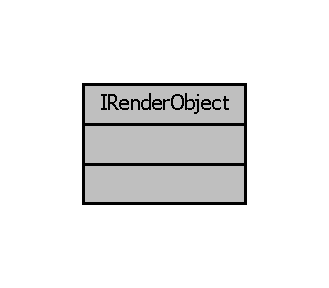
\includegraphics[width=158pt]{d6/dea/classIRenderObject__coll__graph}
\end{center}
\end{figure}


\subsection{Detailed Description}
\begin{DoxyAuthor}{Author}
Marcus Zepp
\end{DoxyAuthor}
\begin{DoxyVersion}{Version}

\end{DoxyVersion}
\begin{DoxyParagraph}{Revision\-:}
1.\-0 
\end{DoxyParagraph}


\begin{DoxyDate}{Date}

\end{DoxyDate}
\begin{DoxyParagraph}{Date\-:}
2014/03/26 14\-:16\-:20 
\end{DoxyParagraph}


Contact\-: {\tt zeppfisj@mailbox.\-tu-\/berlin.\-de} 

The documentation for this class was generated from the following file\-:\begin{DoxyCompactItemize}
\item 
renderobject.\-h\end{DoxyCompactItemize}

\section{Matlab\-Field\-Viewer Class Reference}
\label{classMatlabFieldViewer}\index{Matlab\-Field\-Viewer@{Matlab\-Field\-Viewer}}


{\ttfamily \#include $<$matlabfieldviewer.\-h$>$}



Collaboration diagram for Matlab\-Field\-Viewer\-:
\nopagebreak
\begin{figure}[H]
\begin{center}
\leavevmode
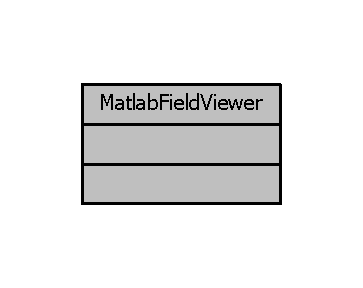
\includegraphics[width=174pt]{d1/d43/classMatlabFieldViewer__coll__graph}
\end{center}
\end{figure}


\subsection{Detailed Description}
\begin{DoxyAuthor}{Author}
Marcus Zepp
\end{DoxyAuthor}
\begin{DoxyVersion}{Version}

\end{DoxyVersion}
\begin{DoxyParagraph}{Revision\-:}
1.\-0 
\end{DoxyParagraph}


\begin{DoxyDate}{Date}

\end{DoxyDate}
\begin{DoxyParagraph}{Date\-:}
2014/03/26 14\-:16\-:20 
\end{DoxyParagraph}


Contact\-: {\tt zeppfisj@mailbox.\-tu-\/berlin.\-de} 

The documentation for this class was generated from the following file\-:\begin{DoxyCompactItemize}
\item 
matlabfieldviewer.\-h\end{DoxyCompactItemize}

\section{sfs\-\_\-visualizer\-:\-:Matlab\-Field\-Viewer Class Reference}
\label{classsfs__visualizer_1_1MatlabFieldViewer}\index{sfs\-\_\-visualizer\-::\-Matlab\-Field\-Viewer@{sfs\-\_\-visualizer\-::\-Matlab\-Field\-Viewer}}


A Field\-Viewer for Matlab files.  




{\ttfamily \#include $<$matlabfieldviewer.\-h$>$}



Inheritance diagram for sfs\-\_\-visualizer\-:\-:Matlab\-Field\-Viewer\-:
\nopagebreak
\begin{figure}[H]
\begin{center}
\leavevmode
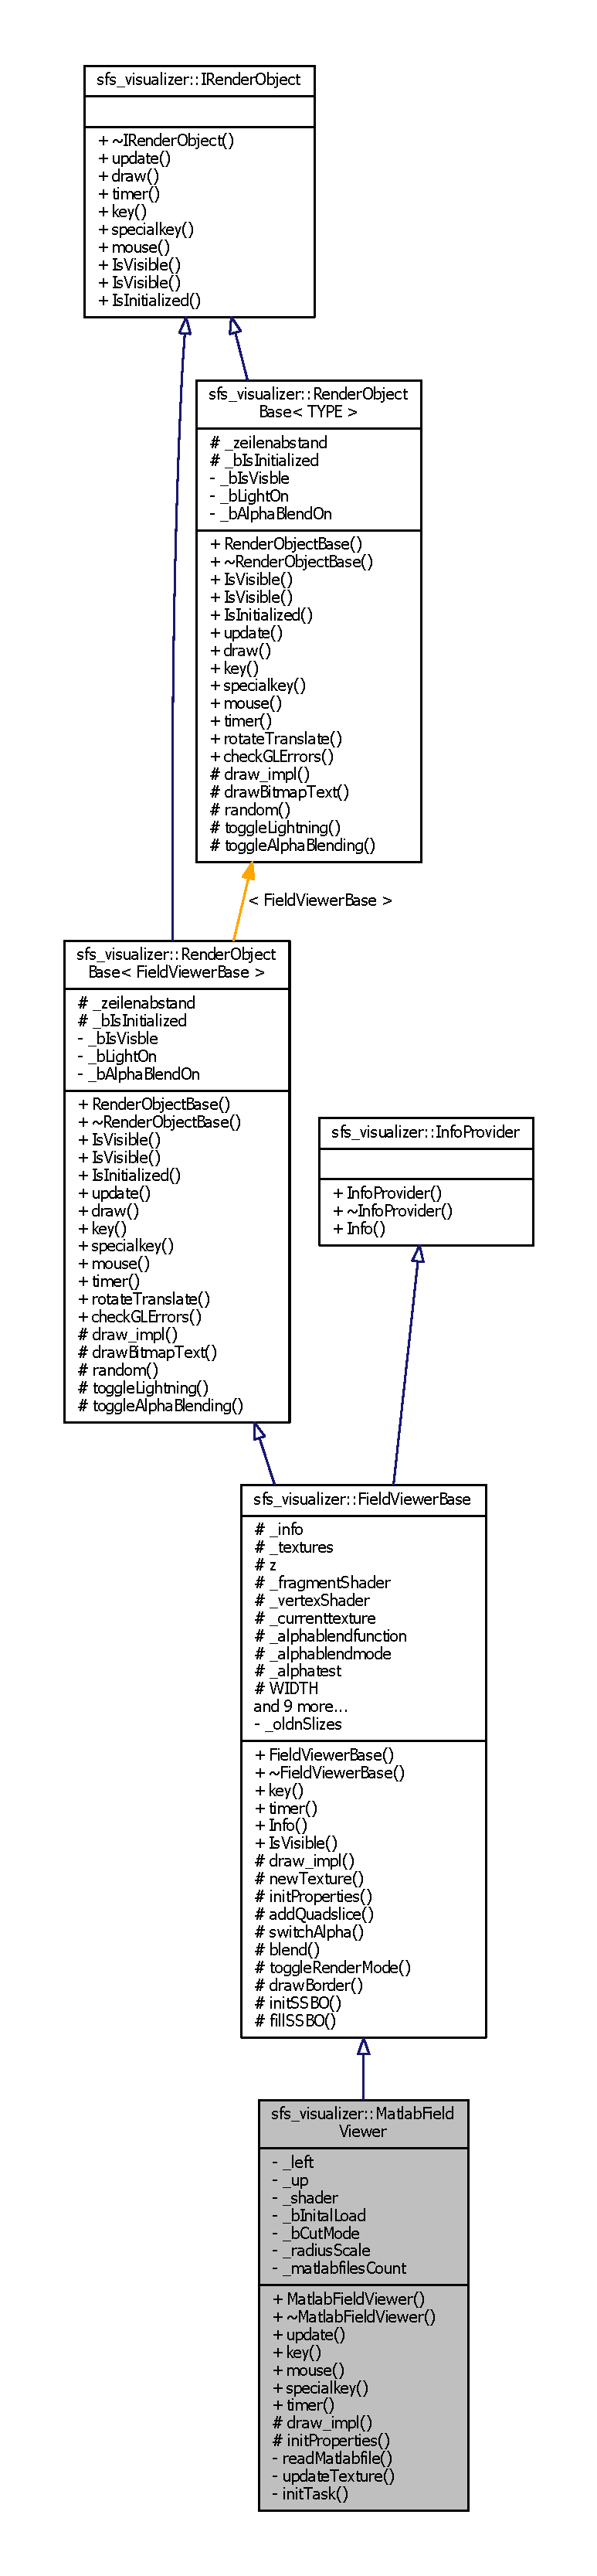
\includegraphics[height=550pt]{df/d65/classsfs__visualizer_1_1MatlabFieldViewer__inherit__graph}
\end{center}
\end{figure}


Collaboration diagram for sfs\-\_\-visualizer\-:\-:Matlab\-Field\-Viewer\-:
\nopagebreak
\begin{figure}[H]
\begin{center}
\leavevmode
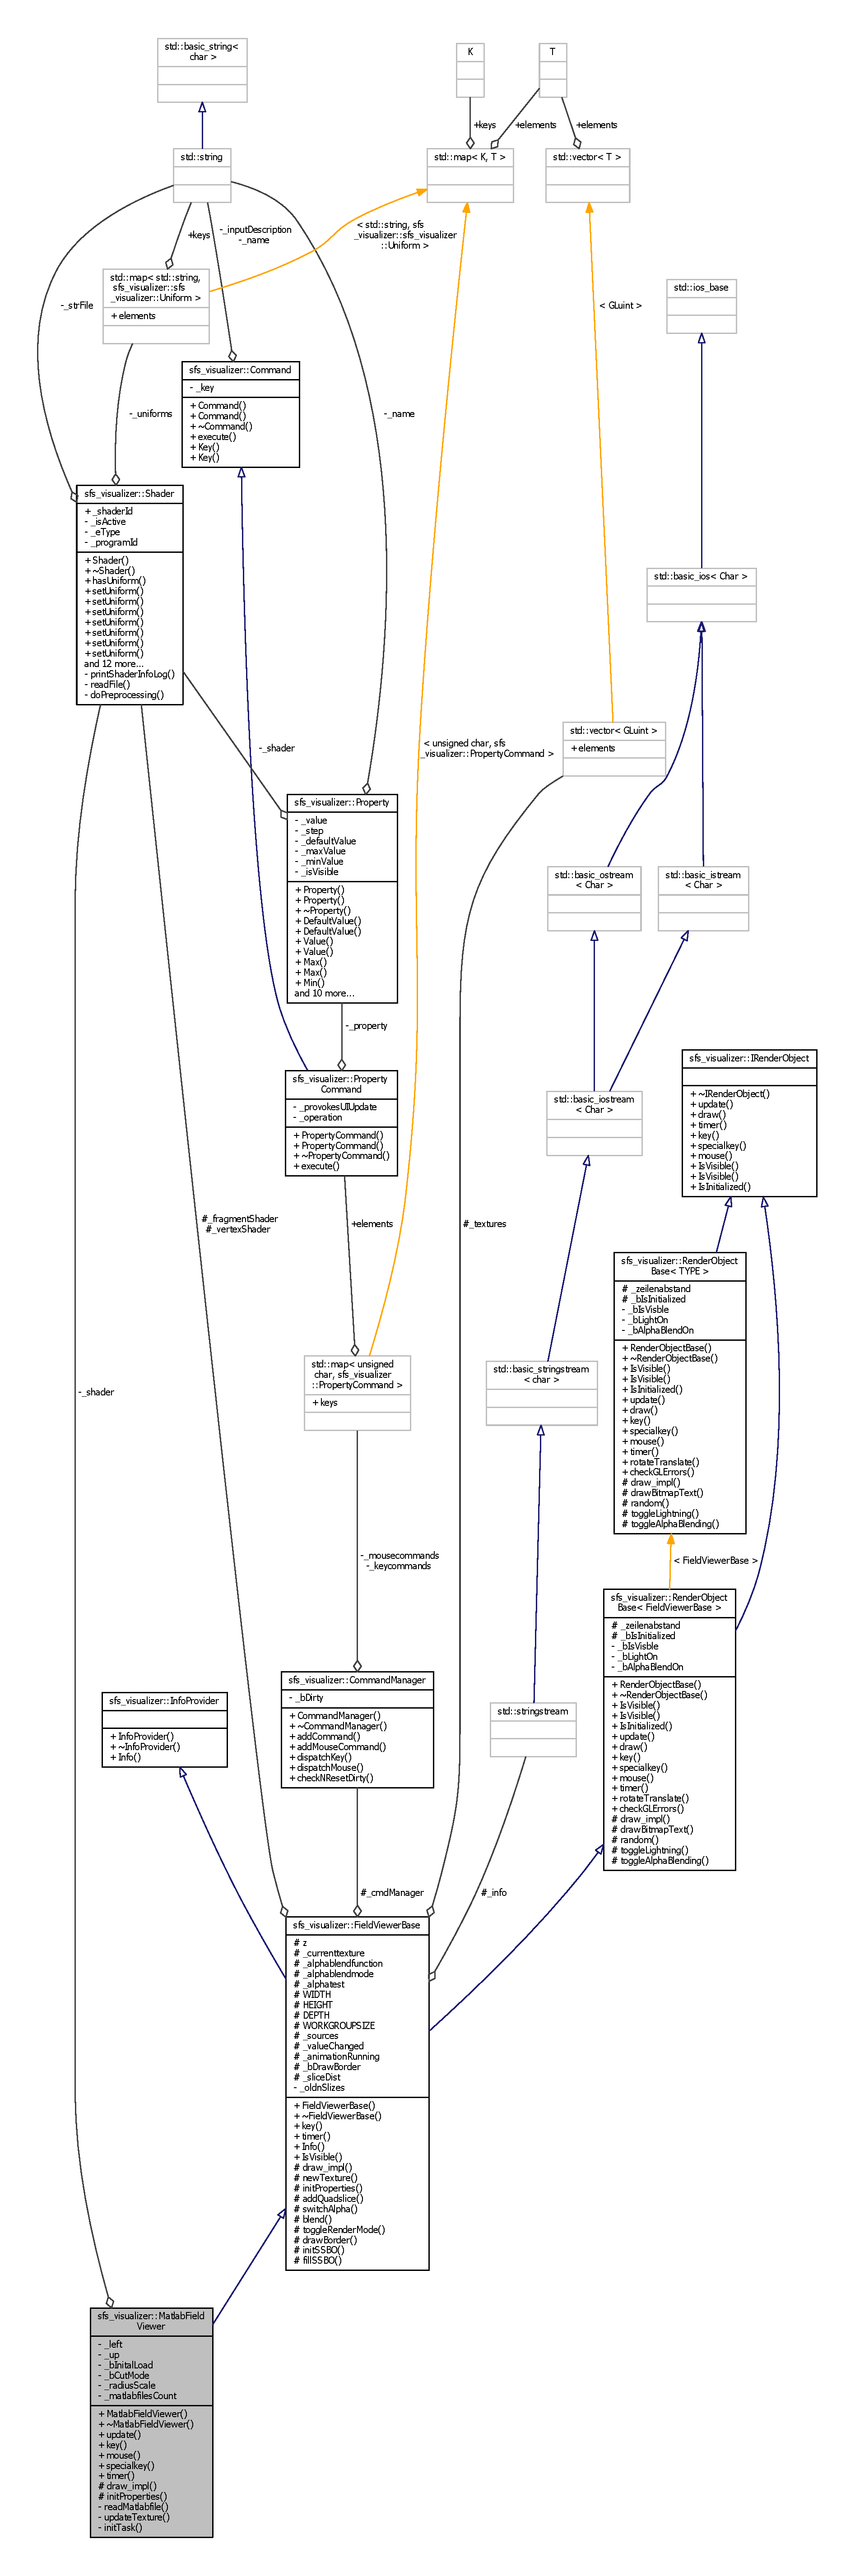
\includegraphics[height=550pt]{d8/da9/classsfs__visualizer_1_1MatlabFieldViewer__coll__graph}
\end{center}
\end{figure}
\subsection*{Public Member Functions}
\begin{DoxyCompactItemize}
\item 
virtual void {\bf update} ()
\begin{DoxyCompactList}\small\item\em methods \end{DoxyCompactList}\item 
virtual void {\bf key} (unsigned char key, int x, int y)
\begin{DoxyCompactList}\small\item\em user inputs \end{DoxyCompactList}\item 
virtual void {\bfseries mouse} (int button, int state, int x, int y)\label{classsfs__visualizer_1_1MatlabFieldViewer_a293d218232886bfb087f7ecf6e5627d8}

\item 
virtual void {\bfseries specialkey} (int {\bf key}, int x, int y)\label{classsfs__visualizer_1_1MatlabFieldViewer_a4112bfbbb13776af8c8265816428ef29}

\item 
virtual void {\bfseries timer} (int update\-Rate\-Ms)\label{classsfs__visualizer_1_1MatlabFieldViewer_a4ff95419bac2526cc95ee386e8d31ca2}

\end{DoxyCompactItemize}
\subsection*{Protected Member Functions}
\begin{DoxyCompactItemize}
\item 
virtual void {\bfseries draw\-\_\-impl} ()\label{classsfs__visualizer_1_1MatlabFieldViewer_ab5f4e4835af3c56da1ca95992a5715ed}

\item 
virtual void {\bfseries init\-Properties} ()\label{classsfs__visualizer_1_1MatlabFieldViewer_a60d6a2d8dce9c40e41bea67b0e513f4c}

\end{DoxyCompactItemize}
\subsection*{Private Member Functions}
\begin{DoxyCompactItemize}
\item 
void {\bfseries read\-Matlabfile} (const char $\ast$file\-\_\-name)\label{classsfs__visualizer_1_1MatlabFieldViewer_a67116af72d447a4de35d32ad5b06ac37}

\item 
void {\bfseries update\-Texture} ()\label{classsfs__visualizer_1_1MatlabFieldViewer_a0948f48965da635cb2cd70fbc5cd02e9}

\item 
void {\bf init\-Task} (boost\-::exception\-\_\-ptr \&error)
\begin{DoxyCompactList}\small\item\em the matlabfile is loaded from a background thread \end{DoxyCompactList}\end{DoxyCompactItemize}
\subsection*{Private Attributes}
\begin{DoxyCompactItemize}
\item 
float {\bfseries \-\_\-left}\label{classsfs__visualizer_1_1MatlabFieldViewer_a6e846f2e9b9736597f0c163c69079673}

\item 
float {\bfseries \-\_\-up}\label{classsfs__visualizer_1_1MatlabFieldViewer_abeef5c9aac4de343e5e635648ea199d1}

\item 
{\bf Shader} $\ast$ {\bfseries \-\_\-shader}\label{classsfs__visualizer_1_1MatlabFieldViewer_ab68454fda33a5458c1277a9dad7396f5}

\item 
bool {\bfseries \-\_\-b\-Inital\-Load}\label{classsfs__visualizer_1_1MatlabFieldViewer_aeaefbb79a71fe1947be644fa4bdfc134}

\item 
bool {\bfseries \-\_\-b\-Cut\-Mode}\label{classsfs__visualizer_1_1MatlabFieldViewer_a79a2b17513fd45c2793b99e169a6314c}

\item 
float {\bfseries \-\_\-radius\-Scale}\label{classsfs__visualizer_1_1MatlabFieldViewer_a2f771173ffc3af881cc97292def7b345}

\item 
int {\bfseries \-\_\-matlabfiles\-Count}\label{classsfs__visualizer_1_1MatlabFieldViewer_a02c8781c52507acea32ef211e172716b}

\end{DoxyCompactItemize}
\subsection*{Additional Inherited Members}


\subsection{Detailed Description}
A Field\-Viewer for Matlab files. 

Definition at line 29 of file matlabfieldviewer.\-h.



\subsection{Member Function Documentation}
\index{sfs\-\_\-visualizer\-::\-Matlab\-Field\-Viewer@{sfs\-\_\-visualizer\-::\-Matlab\-Field\-Viewer}!update@{update}}
\index{update@{update}!sfs_visualizer::MatlabFieldViewer@{sfs\-\_\-visualizer\-::\-Matlab\-Field\-Viewer}}
\subsubsection[{update}]{\setlength{\rightskip}{0pt plus 5cm}void Matlab\-Field\-Viewer\-::update (
\begin{DoxyParamCaption}
{}
\end{DoxyParamCaption}
)\hspace{0.3cm}{\ttfamily [virtual]}}\label{classsfs__visualizer_1_1MatlabFieldViewer_a4997514b7715c83d2c513576af0a2c60}


methods 



Reimplemented from {\bf sfs\-\_\-visualizer\-::\-Render\-Object\-Base$<$ Field\-Viewer\-Base $>$} \doxyref{}{p.}{de/d2a/classsfs__visualizer_1_1RenderObjectBase_aab3270a6296d723574efcebe4d464ba9}.



Definition at line 290 of file matlabfieldviewer.\-cpp.

\index{sfs\-\_\-visualizer\-::\-Matlab\-Field\-Viewer@{sfs\-\_\-visualizer\-::\-Matlab\-Field\-Viewer}!key@{key}}
\index{key@{key}!sfs_visualizer::MatlabFieldViewer@{sfs\-\_\-visualizer\-::\-Matlab\-Field\-Viewer}}
\subsubsection[{key}]{\setlength{\rightskip}{0pt plus 5cm}void Matlab\-Field\-Viewer\-::key (
\begin{DoxyParamCaption}
\item[{unsigned char}]{key, }
\item[{int}]{x, }
\item[{int}]{y}
\end{DoxyParamCaption}
)\hspace{0.3cm}{\ttfamily [virtual]}}\label{classsfs__visualizer_1_1MatlabFieldViewer_aaba2a2a82434165851e44a01f299d58b}


user inputs 



Reimplemented from {\bf sfs\-\_\-visualizer\-::\-Field\-Viewer\-Base} \doxyref{}{p.}{dc/dc0/classsfs__visualizer_1_1FieldViewerBase_acebb098dc25cd342be007c47cc2e64ab}.



Definition at line 166 of file matlabfieldviewer.\-cpp.



References sfs\-\_\-visualizer\-::\-Render\-Object\-Base$<$ Field\-Viewer\-Base $>$\-::\-Is\-Visible(), sfs\-\_\-visualizer\-::\-Render\-Object\-Base$<$ T\-Y\-P\-E $>$\-::\-Is\-Visible(), and sfs\-\_\-visualizer\-::\-Field\-Viewer\-Base\-::key().

\index{sfs\-\_\-visualizer\-::\-Matlab\-Field\-Viewer@{sfs\-\_\-visualizer\-::\-Matlab\-Field\-Viewer}!init\-Task@{init\-Task}}
\index{init\-Task@{init\-Task}!sfs_visualizer::MatlabFieldViewer@{sfs\-\_\-visualizer\-::\-Matlab\-Field\-Viewer}}
\subsubsection[{init\-Task}]{\setlength{\rightskip}{0pt plus 5cm}void Matlab\-Field\-Viewer\-::init\-Task (
\begin{DoxyParamCaption}
\item[{boost\-::exception\-\_\-ptr \&}]{error}
\end{DoxyParamCaption}
)\hspace{0.3cm}{\ttfamily [private]}}\label{classsfs__visualizer_1_1MatlabFieldViewer_a42e16ed2a33558618af417ebb439639c}


the matlabfile is loaded from a background thread 



Definition at line 19 of file matlabfieldviewer.\-cpp.



The documentation for this class was generated from the following files\-:\begin{DoxyCompactItemize}
\item 
matlabfieldviewer.\-h\item 
matlabfieldviewer.\-cpp\end{DoxyCompactItemize}

\section{Matlab\-File\-Adapter Class Reference}
\label{classMatlabFileAdapter}\index{Matlab\-File\-Adapter@{Matlab\-File\-Adapter}}


{\ttfamily \#include $<$matlabfileadapter.\-h$>$}



Collaboration diagram for Matlab\-File\-Adapter\-:
\nopagebreak
\begin{figure}[H]
\begin{center}
\leavevmode
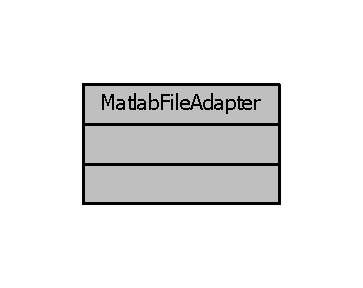
\includegraphics[width=174pt]{d1/d3f/classMatlabFileAdapter__coll__graph}
\end{center}
\end{figure}


\subsection{Detailed Description}
\begin{DoxyAuthor}{Author}
Marcus Zepp
\end{DoxyAuthor}
\begin{DoxyVersion}{Version}

\end{DoxyVersion}
\begin{DoxyParagraph}{Revision\-:}
1.\-0 
\end{DoxyParagraph}


\begin{DoxyDate}{Date}

\end{DoxyDate}
\begin{DoxyParagraph}{Date\-:}
2014/03/26 14\-:16\-:20 
\end{DoxyParagraph}


Contact\-: {\tt zeppfisj@mailbox.\-tu-\/berlin.\-de} 

The documentation for this class was generated from the following file\-:\begin{DoxyCompactItemize}
\item 
matlabfileadapter.\-h\end{DoxyCompactItemize}

\section{sfs\-\_\-visualizer\-:\-:Matlab\-File\-Adapter Class Reference}
\label{classsfs__visualizer_1_1MatlabFileAdapter}\index{sfs\-\_\-visualizer\-::\-Matlab\-File\-Adapter@{sfs\-\_\-visualizer\-::\-Matlab\-File\-Adapter}}


this class uses the matio-\/lib for reading and writing mat-\/files  




{\ttfamily \#include $<$matlabfileadapter.\-h$>$}



Collaboration diagram for sfs\-\_\-visualizer\-:\-:Matlab\-File\-Adapter\-:
\nopagebreak
\begin{figure}[H]
\begin{center}
\leavevmode
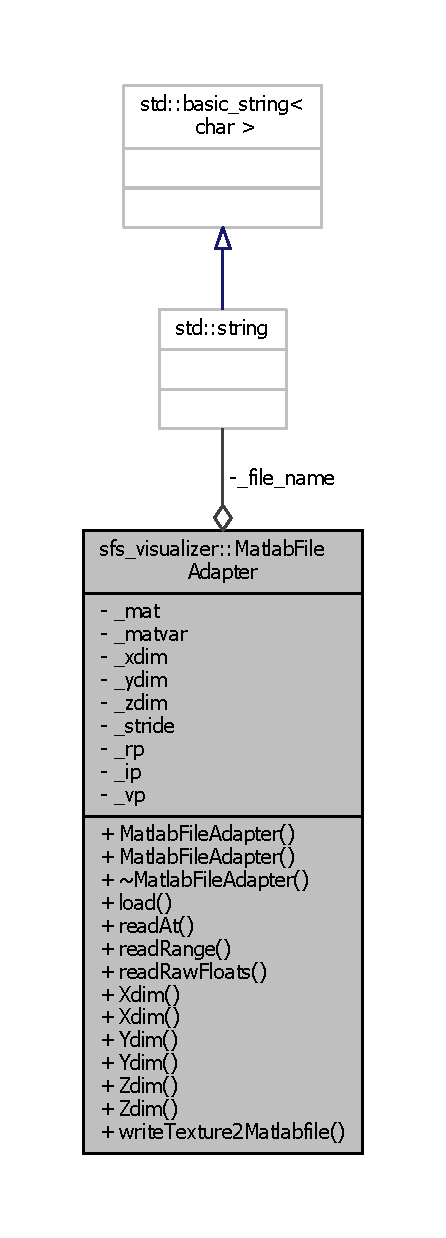
\includegraphics[height=550pt]{d2/d77/classsfs__visualizer_1_1MatlabFileAdapter__coll__graph}
\end{center}
\end{figure}
\subsection*{Public Member Functions}
\begin{DoxyCompactItemize}
\item 
{\bfseries Matlab\-File\-Adapter} (const std\-::string \&file\-\_\-name)\label{classsfs__visualizer_1_1MatlabFileAdapter_a5b4a5db91581955e6063cfcb46a04b78}

\item 
void {\bfseries load} (const std\-::string \&file\-\_\-name)\label{classsfs__visualizer_1_1MatlabFileAdapter_a27ccc22fcca1f3ce06e633fe316f08e8}

\item 
G\-Lfloat {\bfseries read\-At} (int x, int y, int z)\label{classsfs__visualizer_1_1MatlabFileAdapter_abaa83da76f77d8a84d4af2c108ef7592}

\item 
void {\bfseries read\-Range} (int start, int count, G\-Lfloat $\ast$result)\label{classsfs__visualizer_1_1MatlabFileAdapter_ad73cb969daba9a56e8b43fa9e2b7ed19}

\item 
void {\bfseries read\-Raw\-Floats} (G\-Lfloat $\ast$$\ast$result)\label{classsfs__visualizer_1_1MatlabFileAdapter_a550e6a58ec5c6d1624b1b6599ff03f64}

\item 
int {\bfseries Xdim} () const \label{classsfs__visualizer_1_1MatlabFileAdapter_ad3eefbd67759fdffbd9ed68b0337f8e4}

\item 
void {\bfseries Xdim} (int val)\label{classsfs__visualizer_1_1MatlabFileAdapter_a88ca59682939f43f7774d2773989ce5b}

\item 
int {\bfseries Ydim} () const \label{classsfs__visualizer_1_1MatlabFileAdapter_ac495cea835c940f2796054235ffba7d0}

\item 
void {\bfseries Ydim} (int val)\label{classsfs__visualizer_1_1MatlabFileAdapter_abce516b08c67a0e8b0b6380bdcb402aa}

\item 
int {\bfseries Zdim} () const \label{classsfs__visualizer_1_1MatlabFileAdapter_aab3bd245cf446708ce46f9954cd854f5}

\item 
void {\bfseries Zdim} (int val)\label{classsfs__visualizer_1_1MatlabFileAdapter_a2009b0e8e6ee57265d5b0d7e36a8d0c4}

\end{DoxyCompactItemize}
\subsection*{Static Public Member Functions}
\begin{DoxyCompactItemize}
\item 
static void {\bfseries write\-Texture2\-Matlabfile} (G\-Lint texture\-Id, int width, int height, int depth, const std\-::string \&file)\label{classsfs__visualizer_1_1MatlabFileAdapter_af734ded74ae130d9f977046056e27a27}

\end{DoxyCompactItemize}
\subsection*{Private Attributes}
\begin{DoxyCompactItemize}
\item 
const std\-::string \& {\bfseries \-\_\-file\-\_\-name}\label{classsfs__visualizer_1_1MatlabFileAdapter_af4566c4a17dd64fc1462883de4b5f35b}

\item 
mat\-\_\-t $\ast$ {\bfseries \-\_\-mat}\label{classsfs__visualizer_1_1MatlabFileAdapter_a85f895d36b743214832393ceaefd1261}

\item 
matvar\-\_\-t $\ast$ {\bfseries \-\_\-matvar}\label{classsfs__visualizer_1_1MatlabFileAdapter_a69342d92fa7ac756a1aa91bd6564c44a}

\item 
int {\bfseries \-\_\-xdim}\label{classsfs__visualizer_1_1MatlabFileAdapter_a0fb4d69aae12ae3b7a0c0781ab726805}

\item 
int {\bfseries \-\_\-ydim}\label{classsfs__visualizer_1_1MatlabFileAdapter_a63aa2a3584fd8cfad3982bad0b1a6c2c}

\item 
int {\bfseries \-\_\-zdim}\label{classsfs__visualizer_1_1MatlabFileAdapter_a5900871096b21dd6acbd067b15cc244d}

\item 
int {\bfseries \-\_\-stride}\label{classsfs__visualizer_1_1MatlabFileAdapter_a55123110e24559d37b0d79a4cfac8bc4}

\item 
char $\ast$ {\bfseries \-\_\-rp}\label{classsfs__visualizer_1_1MatlabFileAdapter_a6e399cb8ea2d5a74a9ac127a8d3b8b7a}

\item 
char $\ast$ {\bfseries \-\_\-ip}\label{classsfs__visualizer_1_1MatlabFileAdapter_af40a587c27ea5679165857f429ea429a}

\item 
char $\ast$ {\bfseries \-\_\-vp}\label{classsfs__visualizer_1_1MatlabFileAdapter_ab67614dbc44570faea981cd44cb26620}

\end{DoxyCompactItemize}


\subsection{Detailed Description}
this class uses the matio-\/lib for reading and writing mat-\/files 

Definition at line 24 of file matlabfileadapter.\-h.



The documentation for this class was generated from the following files\-:\begin{DoxyCompactItemize}
\item 
matlabfileadapter.\-h\item 
matlabfileadapter.\-cpp\end{DoxyCompactItemize}

\section{sfs\-\_\-visualizer\-:\-:Property Class Reference}
\label{classsfs__visualizer_1_1Property}\index{sfs\-\_\-visualizer\-::\-Property@{sfs\-\_\-visualizer\-::\-Property}}


capsulates a value, that can be modified and saved  




{\ttfamily \#include $<$Property.\-h$>$}



Collaboration diagram for sfs\-\_\-visualizer\-:\-:Property\-:\nopagebreak
\begin{figure}[H]
\begin{center}
\leavevmode
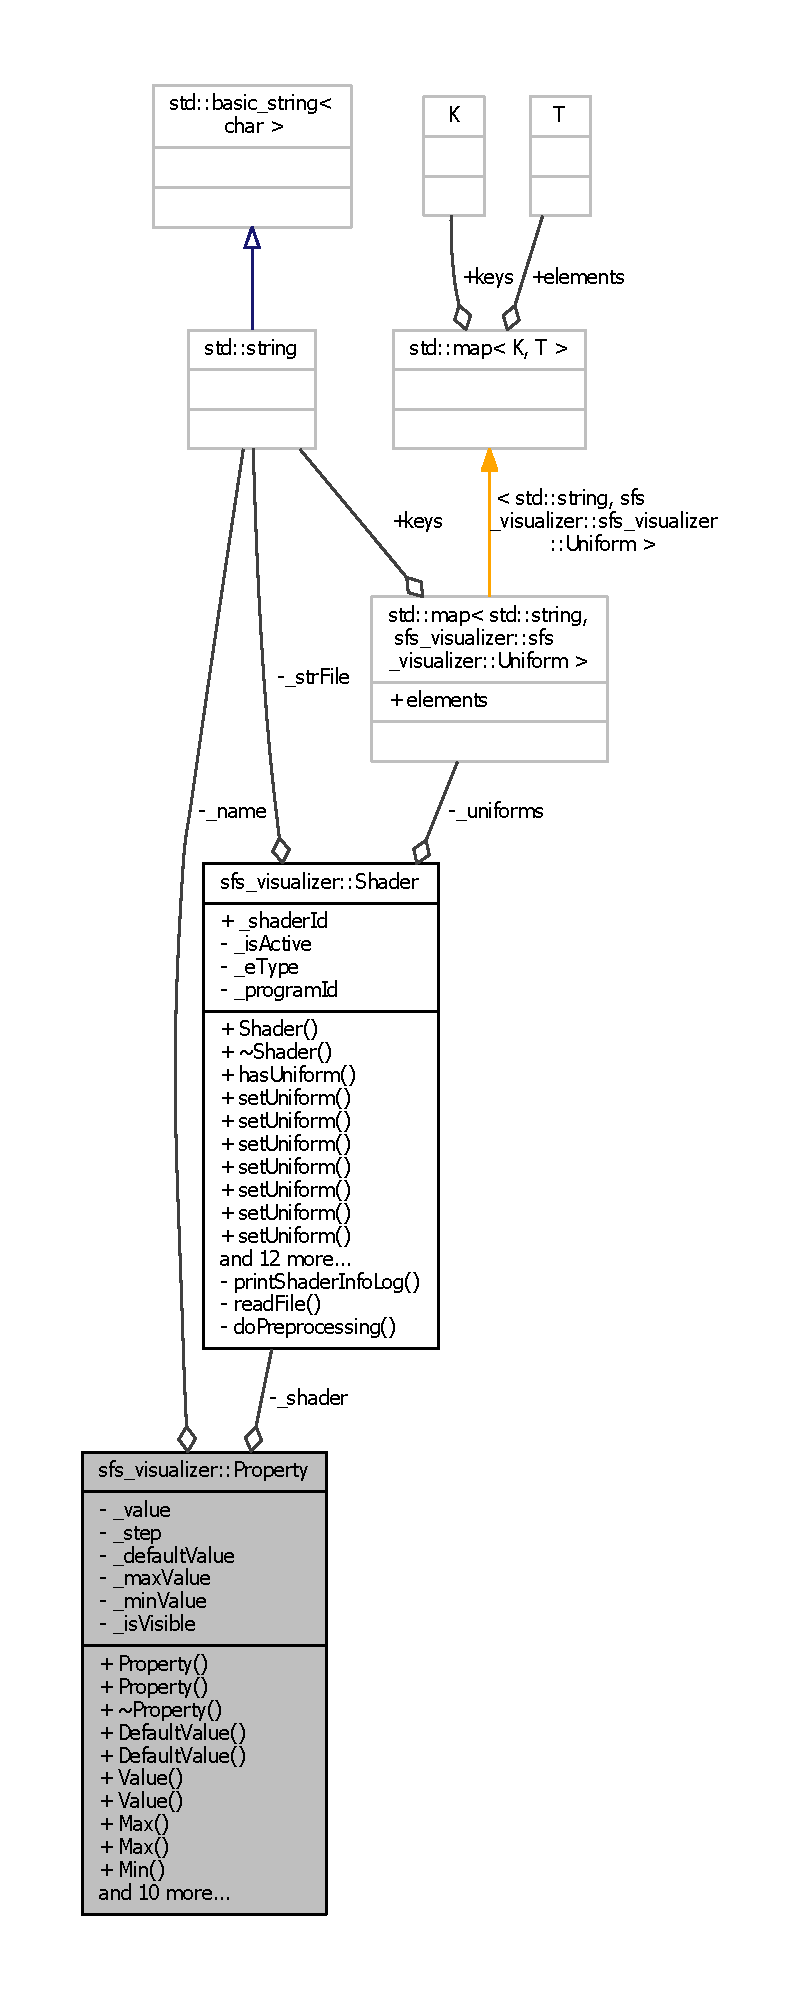
\includegraphics[height=550pt]{d0/d3c/classsfs__visualizer_1_1Property__coll__graph}
\end{center}
\end{figure}
\subsection*{Public Member Functions}
\begin{DoxyCompactItemize}
\item 
{\bfseries Property} (float value, std\-::string name, float step, float default\-Value, {\bf Shader} $\ast$shader=N\-U\-L\-L)\label{classsfs__visualizer_1_1Property_a438d909815621409dbbf1d4591839ae1}

\item 
float {\bfseries Default\-Value} () const \label{classsfs__visualizer_1_1Property_aec431ce75e0047c7ac055a546be758e9}

\item 
void {\bfseries Default\-Value} (float val)\label{classsfs__visualizer_1_1Property_aa76e3a610e0c9cb03e31cbc64310e67c}

\item 
float {\bfseries Value} () const \label{classsfs__visualizer_1_1Property_a71d4855993f1f144f3e19e31d541524c}

\item 
void {\bfseries Value} (float val)\label{classsfs__visualizer_1_1Property_a35ab2d5a595af50d6be37c48c008daa0}

\item 
float {\bfseries Max} () const \label{classsfs__visualizer_1_1Property_aa097088d57b515090065374efd1a5420}

\item 
void {\bfseries Max} (float val)\label{classsfs__visualizer_1_1Property_ace2c6f871b320012fb76831b3cb3afd6}

\item 
float {\bfseries Min} () const \label{classsfs__visualizer_1_1Property_acbd5dbf3f7203857d50f5ff95ae575ee}

\item 
void {\bfseries Min} (float val)\label{classsfs__visualizer_1_1Property_a1077459b26143a72bbaccd34821f3d45}

\item 
std\-::string {\bfseries Name} () const \label{classsfs__visualizer_1_1Property_a0ee3c6cb62b651d697fe2dd441a0506d}

\item 
void {\bfseries Name} (std\-::string val)\label{classsfs__visualizer_1_1Property_aeb9a63ff7b6944d4fe0b65dfc8cc3895}

\item 
float {\bfseries Step} () const \label{classsfs__visualizer_1_1Property_a674f89aee85bf8c24ce5aee71ddb3b4b}

\item 
void {\bfseries Step} (float val)\label{classsfs__visualizer_1_1Property_a8537b944bc4fe8a82e4f8d7a3f5fe981}

\item 
void {\bfseries write\-Shader\-Value} ()\label{classsfs__visualizer_1_1Property_a83a7f12a8cb533032c0723f3a5f58f43}

\item 
void {\bfseries reset\-To\-Default} ()\label{classsfs__visualizer_1_1Property_a3634270ca6989002d26f3f2988914b8f}

\item 
{\bf Shader} $\ast$ {\bfseries get\-Shader} ()\label{classsfs__visualizer_1_1Property_ac2be22856a8d08abdaefbe0140c8e6e8}

\item 
bool {\bfseries Is\-Visible} () const \label{classsfs__visualizer_1_1Property_ab3c00edd610dbfc12915379e5e73b9ad}

\item 
void {\bfseries Is\-Visible} (bool val)\label{classsfs__visualizer_1_1Property_a3fa69ca189e0fadffca0b2305cf6af3a}

\end{DoxyCompactItemize}
\subsection*{Private Attributes}
\begin{DoxyCompactItemize}
\item 
float {\bfseries \-\_\-value}\label{classsfs__visualizer_1_1Property_ad66b33a0c3e739d404e398bc6ffad94d}

\item 
std\-::string {\bfseries \-\_\-name}\label{classsfs__visualizer_1_1Property_a682d86a90812e7a3c15fae98f61a08e4}

\item 
float {\bfseries \-\_\-step}\label{classsfs__visualizer_1_1Property_abbaaffe58bd9f6e8652e909bc8af2ef4}

\item 
float {\bfseries \-\_\-default\-Value}\label{classsfs__visualizer_1_1Property_a29fa42cc26cd53c8647b9b39b8f392ff}

\item 
float {\bfseries \-\_\-max\-Value}\label{classsfs__visualizer_1_1Property_a5b0ba0433a8e113a3f161743ae780ba7}

\item 
float {\bfseries \-\_\-min\-Value}\label{classsfs__visualizer_1_1Property_a86ebd202495edd89e5e927ac03d88616}

\item 
{\bf Shader} $\ast$ {\bfseries \-\_\-shader}\label{classsfs__visualizer_1_1Property_a2ba2422edef8ab50e856625b53b58cd4}

\item 
bool {\bfseries \-\_\-is\-Visible}\label{classsfs__visualizer_1_1Property_a0a15bcdef46072e38b3c019f54e632c2}

\end{DoxyCompactItemize}


\subsection{Detailed Description}
capsulates a value, that can be modified and saved 

Definition at line 26 of file Property.\-h.



The documentation for this class was generated from the following files\-:\begin{DoxyCompactItemize}
\item 
Property.\-h\item 
Property.\-cpp\end{DoxyCompactItemize}

\section{Property Class Reference}
\label{classProperty}\index{Property@{Property}}


{\ttfamily \#include $<$Property.\-h$>$}



Collaboration diagram for Property\-:
\nopagebreak
\begin{figure}[H]
\begin{center}
\leavevmode
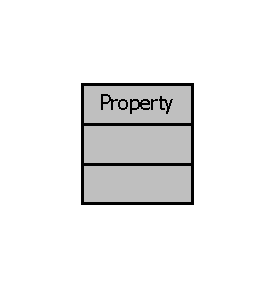
\includegraphics[width=132pt]{d3/dfb/classProperty__coll__graph}
\end{center}
\end{figure}


\subsection{Detailed Description}
\begin{DoxyAuthor}{Author}
Marcus Zepp
\end{DoxyAuthor}
\begin{DoxyVersion}{Version}

\end{DoxyVersion}
\begin{DoxyParagraph}{Revision\-:}
1.\-0 
\end{DoxyParagraph}


\begin{DoxyDate}{Date}

\end{DoxyDate}
\begin{DoxyParagraph}{Date\-:}
2014/03/26 14\-:16\-:20 
\end{DoxyParagraph}


Contact\-: {\tt zeppfisj@mailbox.\-tu-\/berlin.\-de} 

The documentation for this class was generated from the following file\-:\begin{DoxyCompactItemize}
\item 
Property.\-h\end{DoxyCompactItemize}

\section{sfs\-\_\-visualizer\-:\-:Property\-Command Class Reference}
\label{classsfs__visualizer_1_1PropertyCommand}\index{sfs\-\_\-visualizer\-::\-Property\-Command@{sfs\-\_\-visualizer\-::\-Property\-Command}}


This \doxyref{Command}{p.}{d7/d29/classsfs__visualizer_1_1Command} can change \doxyref{Property}{p.}{d4/de7/classsfs__visualizer_1_1Property} values with defined actions eg.  




{\ttfamily \#include $<$command.\-h$>$}



Inheritance diagram for sfs\-\_\-visualizer\-:\-:Property\-Command\-:\nopagebreak
\begin{figure}[H]
\begin{center}
\leavevmode
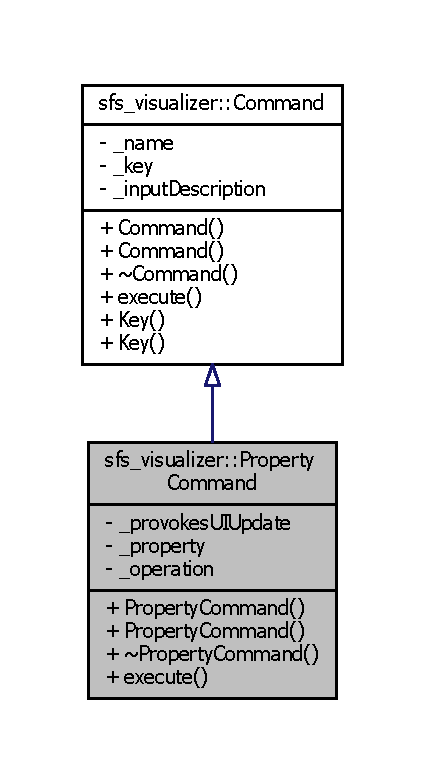
\includegraphics[width=204pt]{d2/dad/classsfs__visualizer_1_1PropertyCommand__inherit__graph}
\end{center}
\end{figure}


Collaboration diagram for sfs\-\_\-visualizer\-:\-:Property\-Command\-:\nopagebreak
\begin{figure}[H]
\begin{center}
\leavevmode
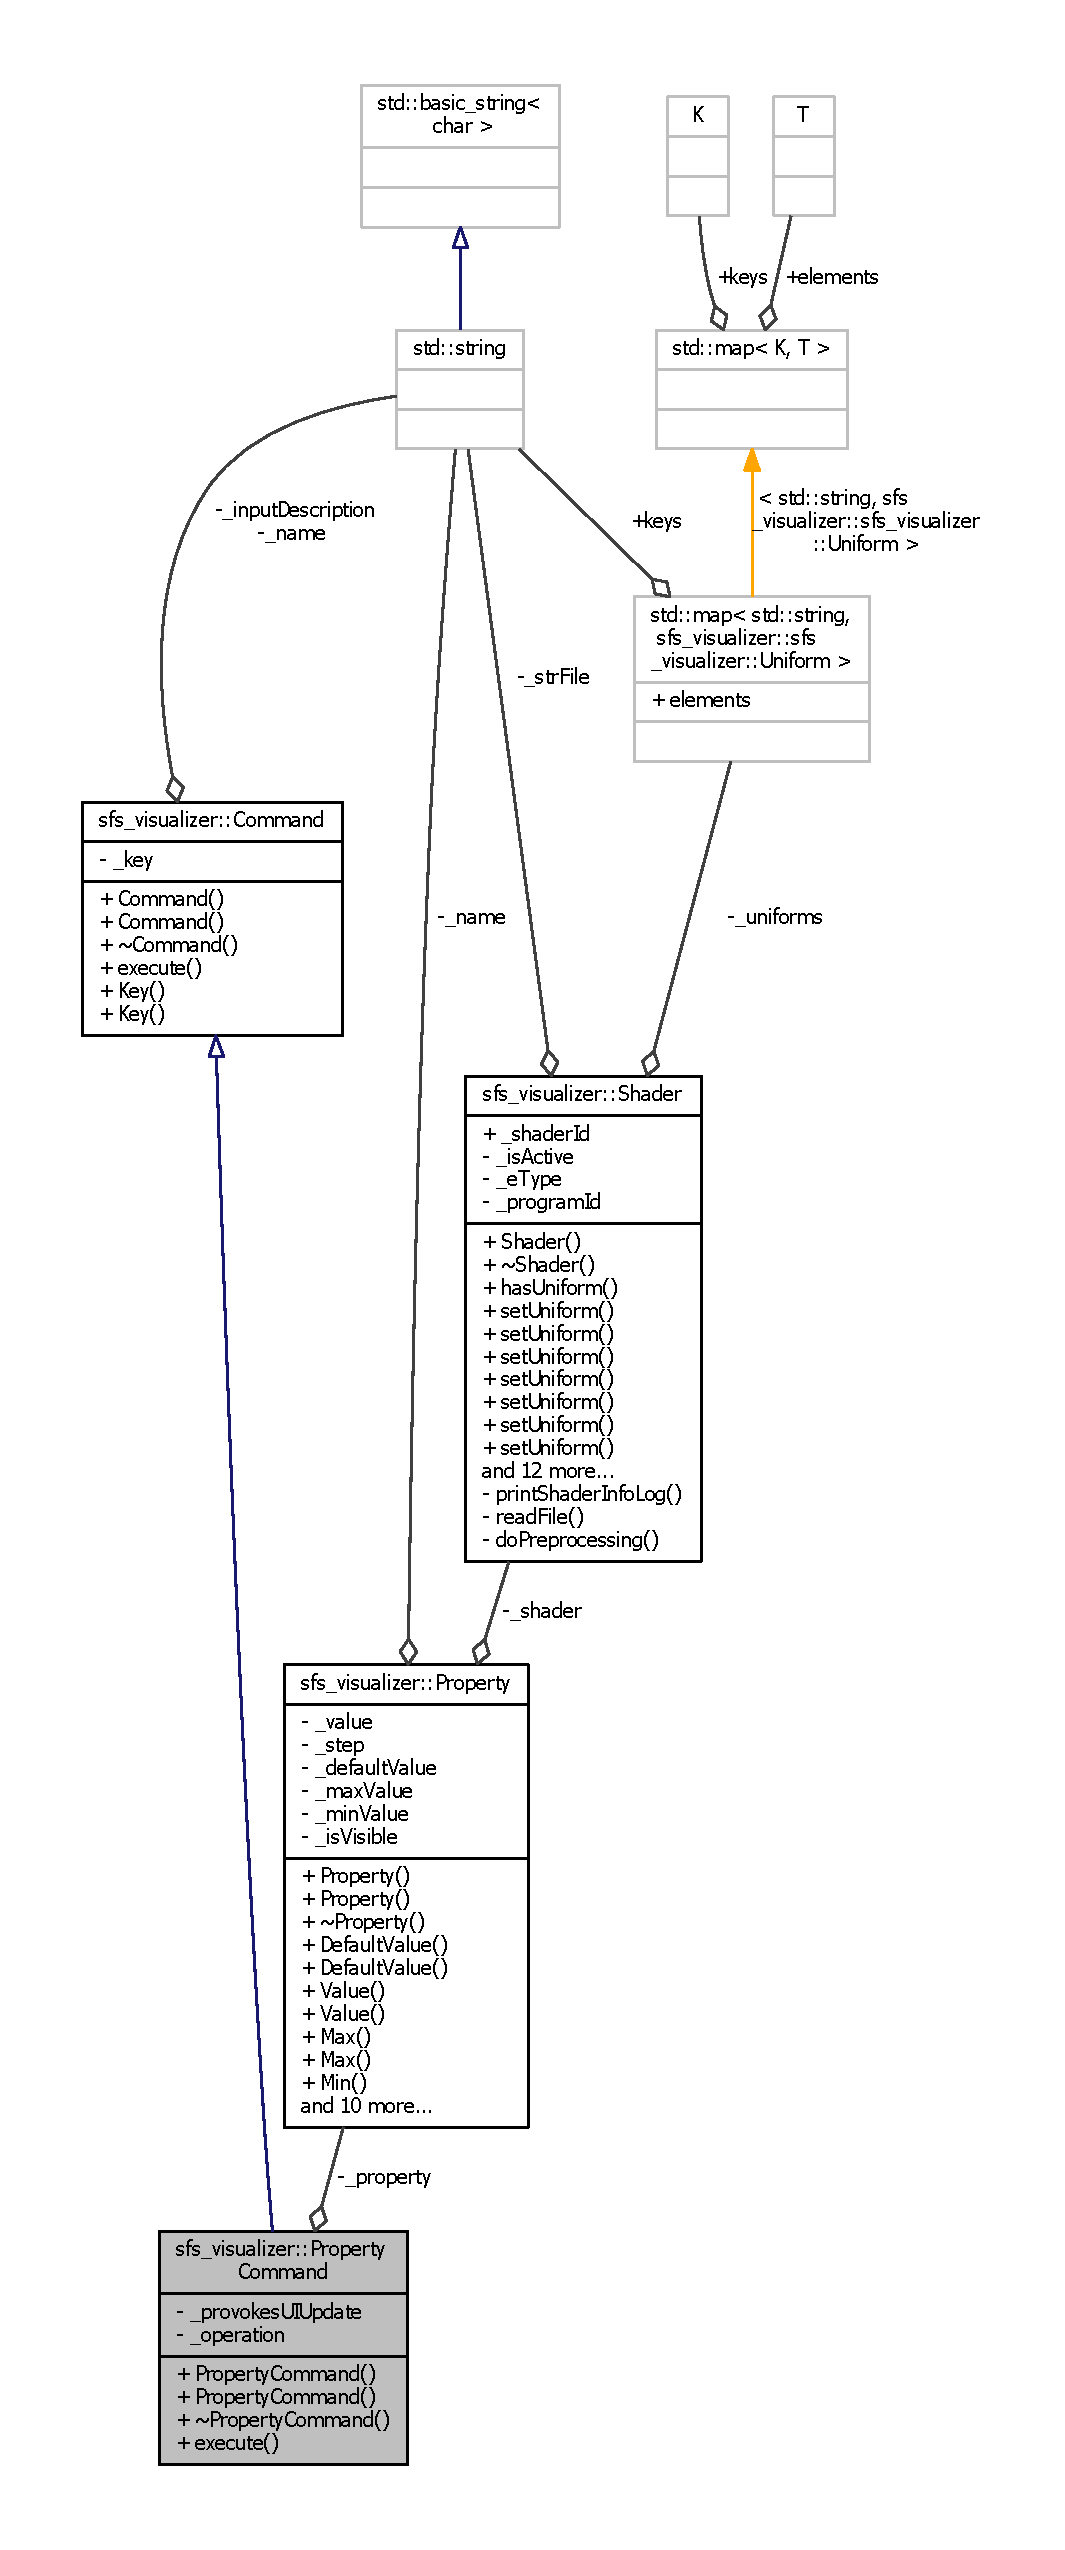
\includegraphics[height=550pt]{de/dec/classsfs__visualizer_1_1PropertyCommand__coll__graph}
\end{center}
\end{figure}
\subsection*{Public Types}
\begin{DoxyCompactItemize}
\item 
enum {\bfseries Operation} \{ \\*
{\bfseries Add}, 
{\bfseries Sub}, 
{\bfseries Mul}, 
{\bfseries Div}, 
\\*
{\bfseries Reset}, 
{\bfseries Toggle}
 \}
\end{DoxyCompactItemize}
\subsection*{Public Member Functions}
\begin{DoxyCompactItemize}
\item 
{\bfseries Property\-Command} (unsigned char key, const std\-::string \&input\-Description, const std\-::string \&name, {\bf Property} \&property, Property\-Command\-::\-Operation operation, bool provokes\-U\-I\-Update=false)\label{classsfs__visualizer_1_1PropertyCommand_aae5b0381272151c39b7a0a0d3bb9683e}

\item 
bool {\bfseries execute} ()\label{classsfs__visualizer_1_1PropertyCommand_a4381b3cc524ca7b4df7ab062cb7e61ae}

\end{DoxyCompactItemize}
\subsection*{Private Attributes}
\begin{DoxyCompactItemize}
\item 
bool {\bfseries \-\_\-provokes\-U\-I\-Update}\label{classsfs__visualizer_1_1PropertyCommand_a1e90773da6a925757ee033dbec8cd78c}

\item 
{\bf Property} \& {\bfseries \-\_\-property}\label{classsfs__visualizer_1_1PropertyCommand_a41e2f9d3877ce440d7eb06db5774ea12}

\item 
Operation {\bfseries \-\_\-operation}\label{classsfs__visualizer_1_1PropertyCommand_a7ba66ab6ebf37effb271fca642ab6710}

\end{DoxyCompactItemize}


\subsection{Detailed Description}
This \doxyref{Command}{p.}{d7/d29/classsfs__visualizer_1_1Command} can change \doxyref{Property}{p.}{d4/de7/classsfs__visualizer_1_1Property} values with defined actions eg. 

Addition, Subtraction etc. 

Definition at line 51 of file command.\-h.



The documentation for this class was generated from the following files\-:\begin{DoxyCompactItemize}
\item 
command.\-h\item 
command.\-cpp\end{DoxyCompactItemize}

\section{Property\-Manager Class Reference}
\label{classPropertyManager}\index{Property\-Manager@{Property\-Manager}}


{\ttfamily \#include $<$propertymanager.\-h$>$}



Collaboration diagram for Property\-Manager\-:
\nopagebreak
\begin{figure}[H]
\begin{center}
\leavevmode
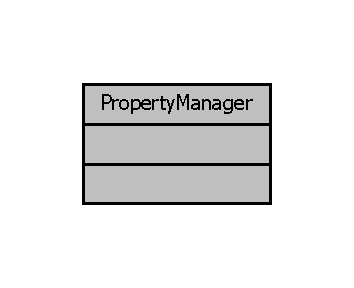
\includegraphics[width=170pt]{df/dc7/classPropertyManager__coll__graph}
\end{center}
\end{figure}


\subsection{Detailed Description}
\begin{DoxyAuthor}{Author}
Marcus Zepp
\end{DoxyAuthor}
\begin{DoxyVersion}{Version}

\end{DoxyVersion}
\begin{DoxyParagraph}{Revision\-:}
1.\-0 
\end{DoxyParagraph}


\begin{DoxyDate}{Date}

\end{DoxyDate}
\begin{DoxyParagraph}{Date\-:}
2014/03/26 14\-:16\-:20 
\end{DoxyParagraph}


Contact\-: {\tt zeppfisj@mailbox.\-tu-\/berlin.\-de} 

The documentation for this class was generated from the following file\-:\begin{DoxyCompactItemize}
\item 
propertymanager.\-h\end{DoxyCompactItemize}

\section{sfs\-\_\-visualizer\-:\-:Property\-Manager Class Reference}
\label{classsfs__visualizer_1_1PropertyManager}\index{sfs\-\_\-visualizer\-::\-Property\-Manager@{sfs\-\_\-visualizer\-::\-Property\-Manager}}


A singletonclass for managing the properties and settings.  




{\ttfamily \#include $<$propertymanager.\-h$>$}



Collaboration diagram for sfs\-\_\-visualizer\-:\-:Property\-Manager\-:\nopagebreak
\begin{figure}[H]
\begin{center}
\leavevmode
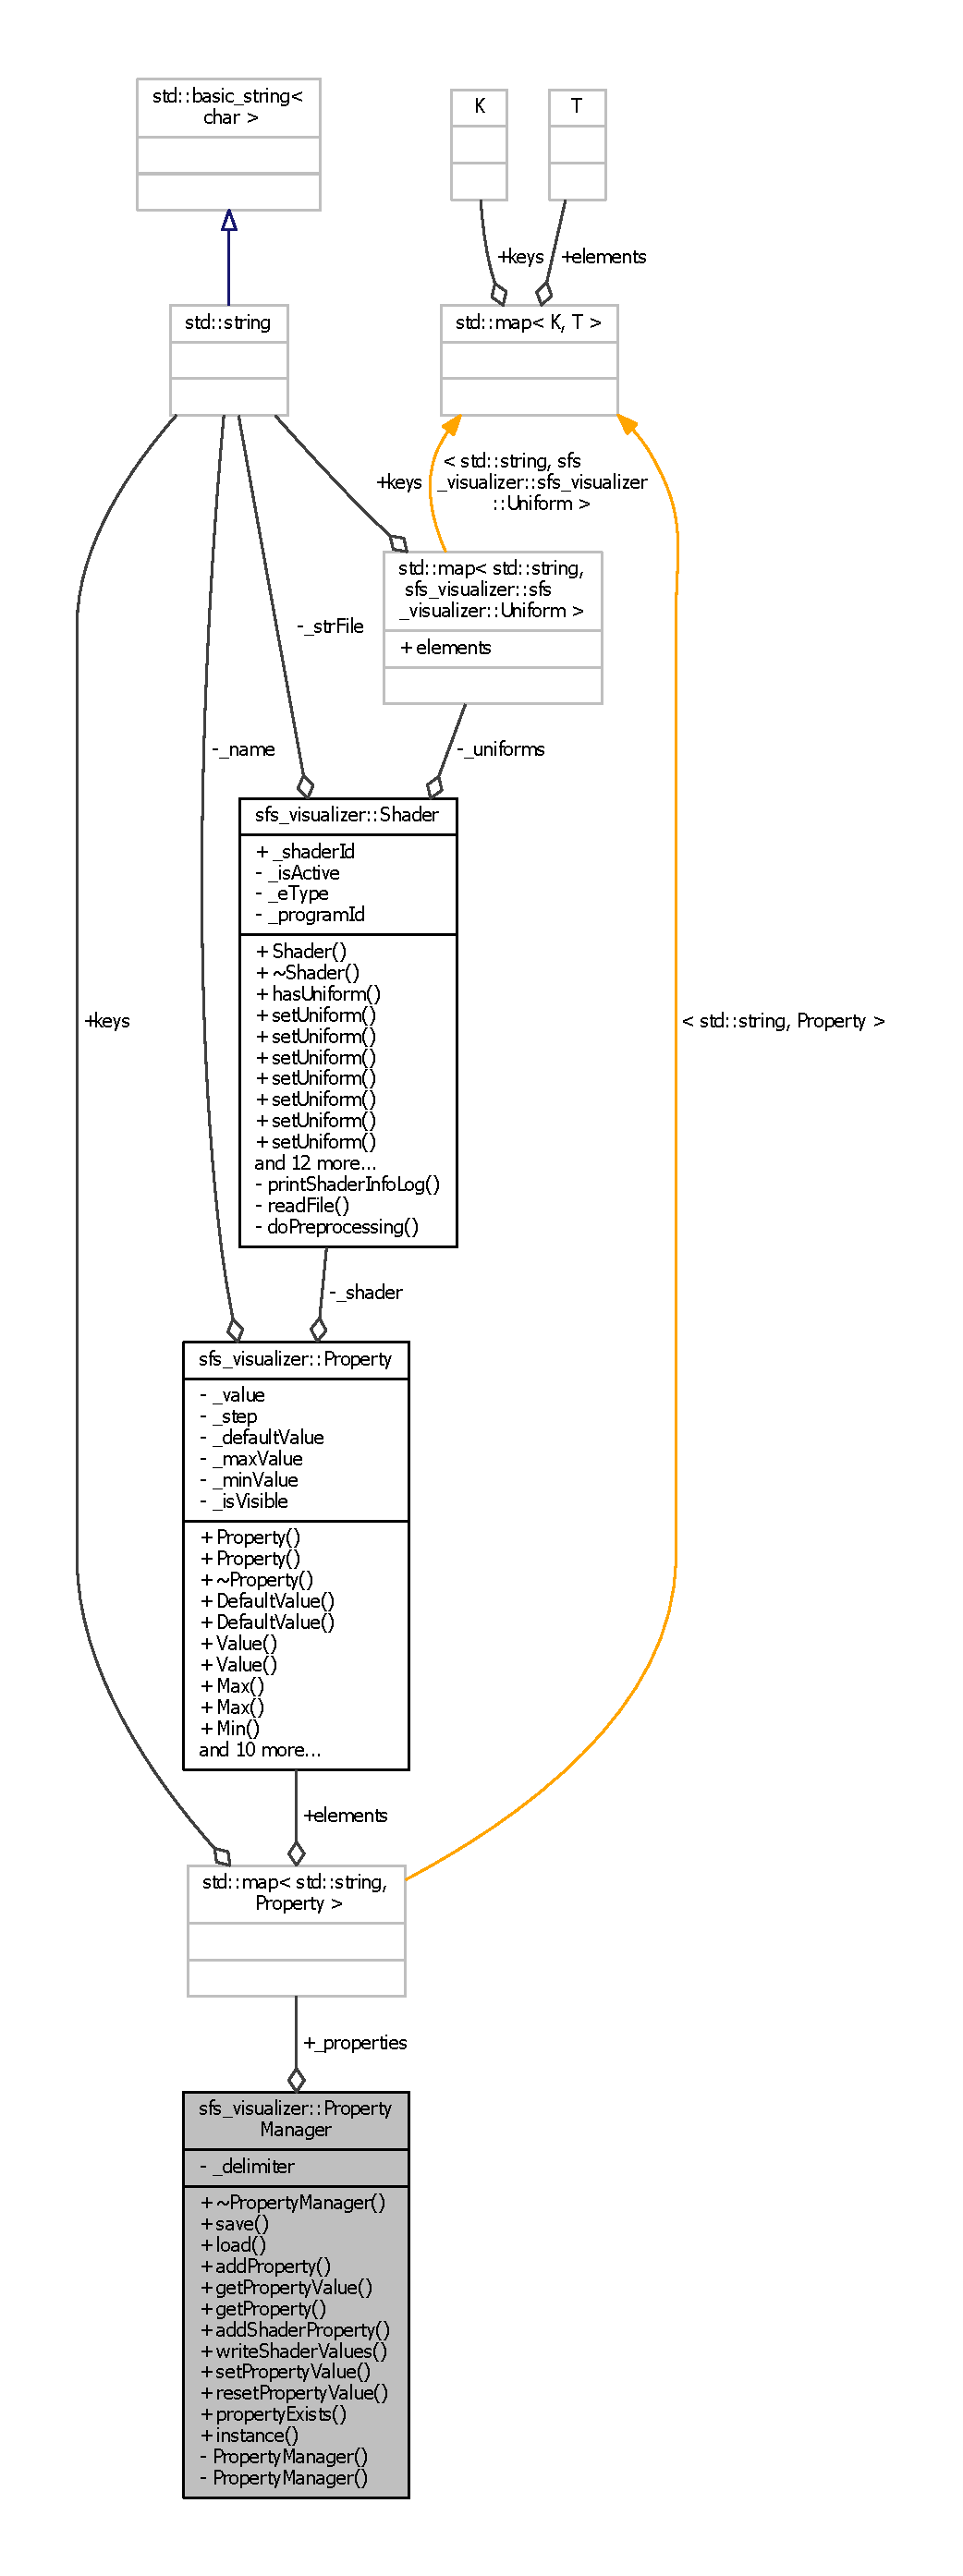
\includegraphics[height=550pt]{db/dd4/classsfs__visualizer_1_1PropertyManager__coll__graph}
\end{center}
\end{figure}
\subsection*{Public Member Functions}
\begin{DoxyCompactItemize}
\item 
void {\bfseries save} ()\label{classsfs__visualizer_1_1PropertyManager_a3087ec9d3a94005856ace0297681fd0a}

\item 
void {\bfseries load} ()\label{classsfs__visualizer_1_1PropertyManager_a87bf025c3c2b5e8a81d5261c1d73e09d}

\item 
{\bf Property} \& {\bfseries add\-Property} (const std\-::string \&name, float default\-Value)\label{classsfs__visualizer_1_1PropertyManager_a618f5d0fb17a08ec5d80037094fff6d4}

\item 
float {\bfseries get\-Property\-Value} (const std\-::string \&name)\label{classsfs__visualizer_1_1PropertyManager_ae480b59e859ff350a0a3fad059b4c290}

\item 
{\bf Property} \& {\bfseries get\-Property} (const std\-::string \&name)\label{classsfs__visualizer_1_1PropertyManager_ab49b96d6505e30b658016798bfef1a87}

\item 
{\bf Property} \& {\bfseries add\-Shader\-Property} (const std\-::string \&name, float default\-Value, {\bf Shader} $\ast$\-\_\-shader)\label{classsfs__visualizer_1_1PropertyManager_a834cb4754f9f2ba229065656aa4eaf4a}

\item 
void {\bfseries write\-Shader\-Values} ({\bf Shader} $\ast$active\-Shader)\label{classsfs__visualizer_1_1PropertyManager_a18e78e31a6c5f6452fba1b1f13a8a3d9}

\item 
void {\bfseries set\-Property\-Value} (const std\-::string \&name, float val)\label{classsfs__visualizer_1_1PropertyManager_af63a1e6ff79a0b4e3623190d592c042d}

\item 
void {\bfseries reset\-Property\-Value} (const std\-::string \&name)\label{classsfs__visualizer_1_1PropertyManager_ac85444bdaeda56ad871f396e9ad2a2bf}

\item 
bool {\bfseries property\-Exists} (const std\-::string \&name) const \label{classsfs__visualizer_1_1PropertyManager_acf619e3ffa40610384545f1865dc460d}

\end{DoxyCompactItemize}
\subsection*{Static Public Member Functions}
\begin{DoxyCompactItemize}
\item 
static {\bf Property\-Manager} \& {\bfseries instance} ()\label{classsfs__visualizer_1_1PropertyManager_a306ceed7e3dee0ac55a0f8248c796e26}

\end{DoxyCompactItemize}
\subsection*{Public Attributes}
\begin{DoxyCompactItemize}
\item 
Property\-Map {\bfseries \-\_\-properties}\label{classsfs__visualizer_1_1PropertyManager_a8d38fb0419d09a948cf3b796a4118a8a}

\end{DoxyCompactItemize}
\subsection*{Private Member Functions}
\begin{DoxyCompactItemize}
\item 
{\bfseries Property\-Manager} (const {\bf Property\-Manager} \&)\label{classsfs__visualizer_1_1PropertyManager_a7aed06263d25b69b4004c253a2edf6fa}

\end{DoxyCompactItemize}
\subsection*{Private Attributes}
\begin{DoxyCompactItemize}
\item 
char {\bfseries \-\_\-delimiter}\label{classsfs__visualizer_1_1PropertyManager_a98d71695ff7a18e4721d06f8637fbd12}

\end{DoxyCompactItemize}


\subsection{Detailed Description}
A singletonclass for managing the properties and settings. 

Definition at line 30 of file propertymanager.\-h.



The documentation for this class was generated from the following files\-:\begin{DoxyCompactItemize}
\item 
propertymanager.\-h\item 
propertymanager.\-cpp\end{DoxyCompactItemize}

\section{sfs\-\_\-visualizer\-:\-:Render\-Engine Class Reference}
\label{classsfs__visualizer_1_1RenderEngine}\index{sfs\-\_\-visualizer\-::\-Render\-Engine@{sfs\-\_\-visualizer\-::\-Render\-Engine}}


responsible for displaying and managing Render\-Objects.  




{\ttfamily \#include $<$renderengine.\-h$>$}



Collaboration diagram for sfs\-\_\-visualizer\-:\-:Render\-Engine\-:\nopagebreak
\begin{figure}[H]
\begin{center}
\leavevmode
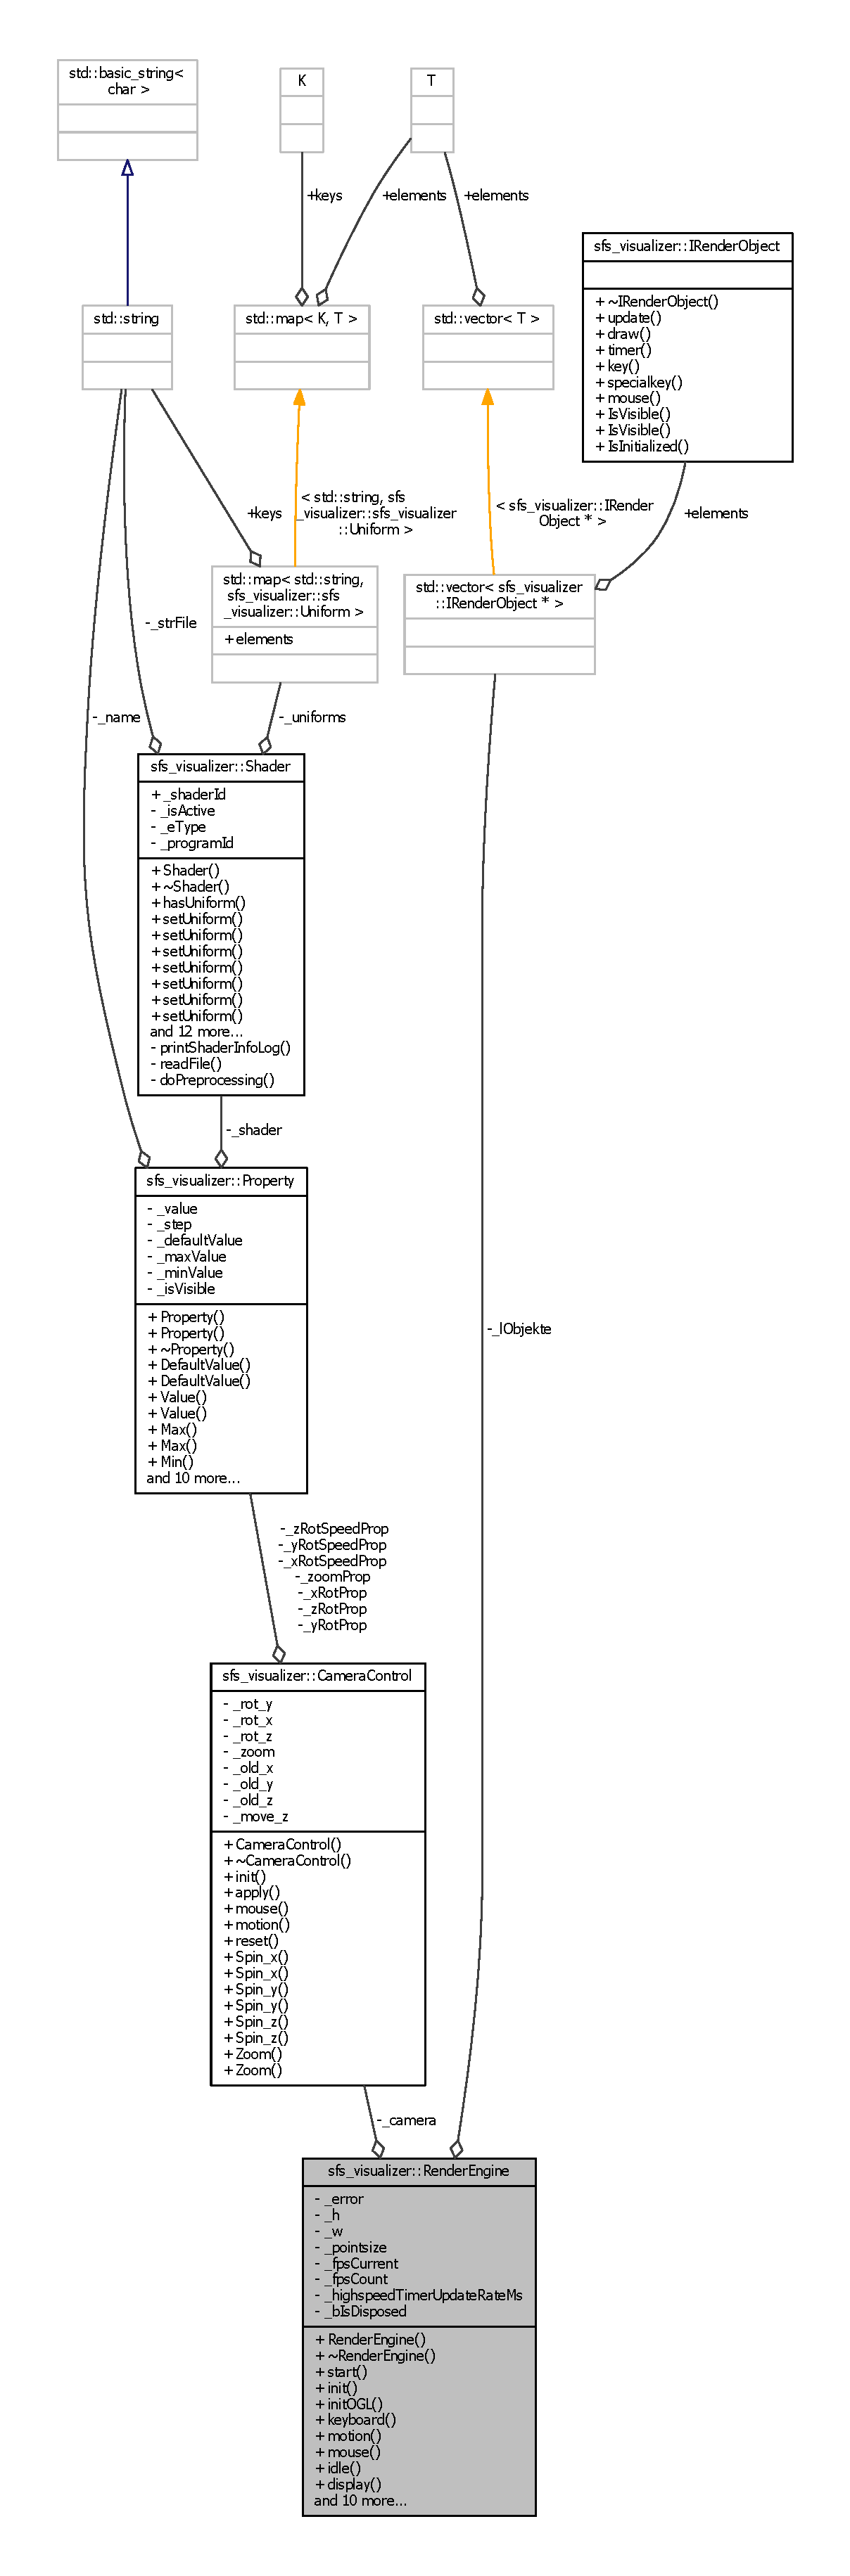
\includegraphics[height=550pt]{d9/d96/classsfs__visualizer_1_1RenderEngine__coll__graph}
\end{center}
\end{figure}
\subsection*{Public Member Functions}
\begin{DoxyCompactItemize}
\item 
void {\bfseries start} ()\label{classsfs__visualizer_1_1RenderEngine_ad64b2eeeaa4aa3bccf825a1d9d00ba86}

\item 
void {\bfseries init} (void)\label{classsfs__visualizer_1_1RenderEngine_a000b228aabf54650392bf2daf9bed0ca}

\item 
void {\bfseries init\-O\-G\-L} ()\label{classsfs__visualizer_1_1RenderEngine_a9e30c9dbd1dbcd52a3192713cb18996a}

\item 
void {\bfseries keyboard} (unsigned char key, int x, int y)\label{classsfs__visualizer_1_1RenderEngine_a12449b504614e6242dac7d1d7bed2c88}

\item 
void {\bfseries motion} (int x, int y)\label{classsfs__visualizer_1_1RenderEngine_a1ddc8839474416f20803c8ef78431986}

\item 
void {\bfseries mouse} (int button, int state, int x, int y)\label{classsfs__visualizer_1_1RenderEngine_afb8308be0bbb12117e053034282f7778}

\item 
void {\bfseries idle} (void)\label{classsfs__visualizer_1_1RenderEngine_aa44da03ff2d1ed4c273a862b19899744}

\item 
void {\bfseries display} (void)\label{classsfs__visualizer_1_1RenderEngine_ac7f71c6329b5f96565a75dfc435c5646}

\item 
void {\bfseries reshape} (int width, int height)\label{classsfs__visualizer_1_1RenderEngine_aa6730eecfe6bdee9788cee9b52445a74}

\item 
void {\bfseries end} (int code)\label{classsfs__visualizer_1_1RenderEngine_a16c1c8a6ae24a9b2f5fe38eba5a068a2}

\item 
void {\bfseries specialkey} (int key, int x, int y)\label{classsfs__visualizer_1_1RenderEngine_a21807d4b8c6c6e6c299446f849b78ba2}

\item 
void {\bfseries timer} (int val)\label{classsfs__visualizer_1_1RenderEngine_a11d5241a901440fd316627663461ad36}

\item 
void {\bfseries highspeedtimer} (int val)\label{classsfs__visualizer_1_1RenderEngine_a398a0c9a6afb6b59e2d0914f1d85e8dc}

\item 
void {\bfseries take\-Screenshot} ()\label{classsfs__visualizer_1_1RenderEngine_a143b5b846ac5622cf3981ba846e3e414}

\item 
void {\bfseries shutdown} ()\label{classsfs__visualizer_1_1RenderEngine_a2e2a2ee4bdc6f9e3a13a7570b0d577c0}

\item 
int {\bf Height} () const 
\begin{DoxyCompactList}\small\item\em mutators and informators \end{DoxyCompactList}\item 
int {\bfseries Width} () const \label{classsfs__visualizer_1_1RenderEngine_a14ae2c2a922499bedfb92a3870962531}

\item 
{\bf sfs\-\_\-visualizer\-::\-Camera\-Control} {\bfseries Camera} () const \label{classsfs__visualizer_1_1RenderEngine_a85627302dc9b06336a064a621fad5543}

\end{DoxyCompactItemize}
\subsection*{Private Attributes}
\begin{DoxyCompactItemize}
\item 
boost\-::exception\-\_\-ptr {\bfseries \-\_\-error}\label{classsfs__visualizer_1_1RenderEngine_ab5d0db5b3e5a6ae7f4a86c572e34600c}

\item 
int {\bfseries \-\_\-h}\label{classsfs__visualizer_1_1RenderEngine_a125284f755dac513f03de2815f9b6efe}

\item 
int {\bfseries \-\_\-w}\label{classsfs__visualizer_1_1RenderEngine_a757f565a1e8fe23cde41da1040f65a47}

\item 
float {\bfseries \-\_\-pointsize}\label{classsfs__visualizer_1_1RenderEngine_a8b2f772a985c77434922ec92f1a88dbe}

\item 
std\-::vector$<$ {\bf I\-Render\-Object} $\ast$ $>$ {\bfseries \-\_\-l\-Objekte}\label{classsfs__visualizer_1_1RenderEngine_aea1c5532fff65d98e86905bf5d810710}

\item 
{\bf Camera\-Control} {\bfseries \-\_\-camera}\label{classsfs__visualizer_1_1RenderEngine_aa6827702371b2b20b13adeb3dd3099fd}

\item 
unsigned int {\bfseries \-\_\-fps\-Current}\label{classsfs__visualizer_1_1RenderEngine_a20d49741071af2558526c9f81ae7349f}

\item 
unsigned int {\bfseries \-\_\-fps\-Count}\label{classsfs__visualizer_1_1RenderEngine_ade82bb4301cfd607386ce6c895724683}

\item 
unsigned int {\bfseries \-\_\-highspeed\-Timer\-Update\-Rate\-Ms}\label{classsfs__visualizer_1_1RenderEngine_ace032ad32dfb12a89f8aecb3ad0effa8}

\item 
bool {\bfseries \-\_\-b\-Is\-Disposed}\label{classsfs__visualizer_1_1RenderEngine_a61ad3dbc71432f261630d639debc061b}

\end{DoxyCompactItemize}


\subsection{Detailed Description}
responsible for displaying and managing Render\-Objects. 

It also dispatches userinputs 

Definition at line 27 of file renderengine.\-h.



\subsection{Member Function Documentation}
\index{sfs\-\_\-visualizer\-::\-Render\-Engine@{sfs\-\_\-visualizer\-::\-Render\-Engine}!Height@{Height}}
\index{Height@{Height}!sfs_visualizer::RenderEngine@{sfs\-\_\-visualizer\-::\-Render\-Engine}}
\subsubsection[{Height}]{\setlength{\rightskip}{0pt plus 5cm}int sfs\-\_\-visualizer\-::\-Render\-Engine\-::\-Height (
\begin{DoxyParamCaption}
{}
\end{DoxyParamCaption}
) const\hspace{0.3cm}{\ttfamily [inline]}}\label{classsfs__visualizer_1_1RenderEngine_a862b56f606a86b9f666f593194e959e9}


mutators and informators 



Definition at line 52 of file renderengine.\-h.



The documentation for this class was generated from the following files\-:\begin{DoxyCompactItemize}
\item 
renderengine.\-h\item 
renderengine.\-cpp\end{DoxyCompactItemize}

\section{Render\-Engine Class Reference}
\label{classRenderEngine}\index{Render\-Engine@{Render\-Engine}}


{\ttfamily \#include $<$renderengine.\-h$>$}



Collaboration diagram for Render\-Engine\-:
\nopagebreak
\begin{figure}[H]
\begin{center}
\leavevmode
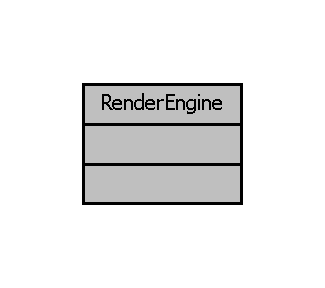
\includegraphics[width=156pt]{d3/d25/classRenderEngine__coll__graph}
\end{center}
\end{figure}


\subsection{Detailed Description}
\begin{DoxyAuthor}{Author}
Marcus Zepp
\end{DoxyAuthor}
\begin{DoxyVersion}{Version}

\end{DoxyVersion}
\begin{DoxyParagraph}{Revision\-:}
1.\-0 
\end{DoxyParagraph}


\begin{DoxyDate}{Date}

\end{DoxyDate}
\begin{DoxyParagraph}{Date\-:}
2014/03/26 14\-:16\-:20 
\end{DoxyParagraph}


Contact\-: {\tt zeppfisj@mailbox.\-tu-\/berlin.\-de} 

The documentation for this class was generated from the following file\-:\begin{DoxyCompactItemize}
\item 
renderengine.\-h\end{DoxyCompactItemize}

\section{sfs\-\_\-visualizer\-:\-:Render\-Object\-Base$<$ T\-Y\-P\-E $>$ Class Template Reference}
\label{classsfs__visualizer_1_1RenderObjectBase}\index{sfs\-\_\-visualizer\-::\-Render\-Object\-Base$<$ T\-Y\-P\-E $>$@{sfs\-\_\-visualizer\-::\-Render\-Object\-Base$<$ T\-Y\-P\-E $>$}}


Base for Render\-Objects, which are objects, that can be shown in 3\-D.  




{\ttfamily \#include $<$renderobjectbase.\-h$>$}



Inheritance diagram for sfs\-\_\-visualizer\-:\-:Render\-Object\-Base$<$ T\-Y\-P\-E $>$\-:
\nopagebreak
\begin{figure}[H]
\begin{center}
\leavevmode
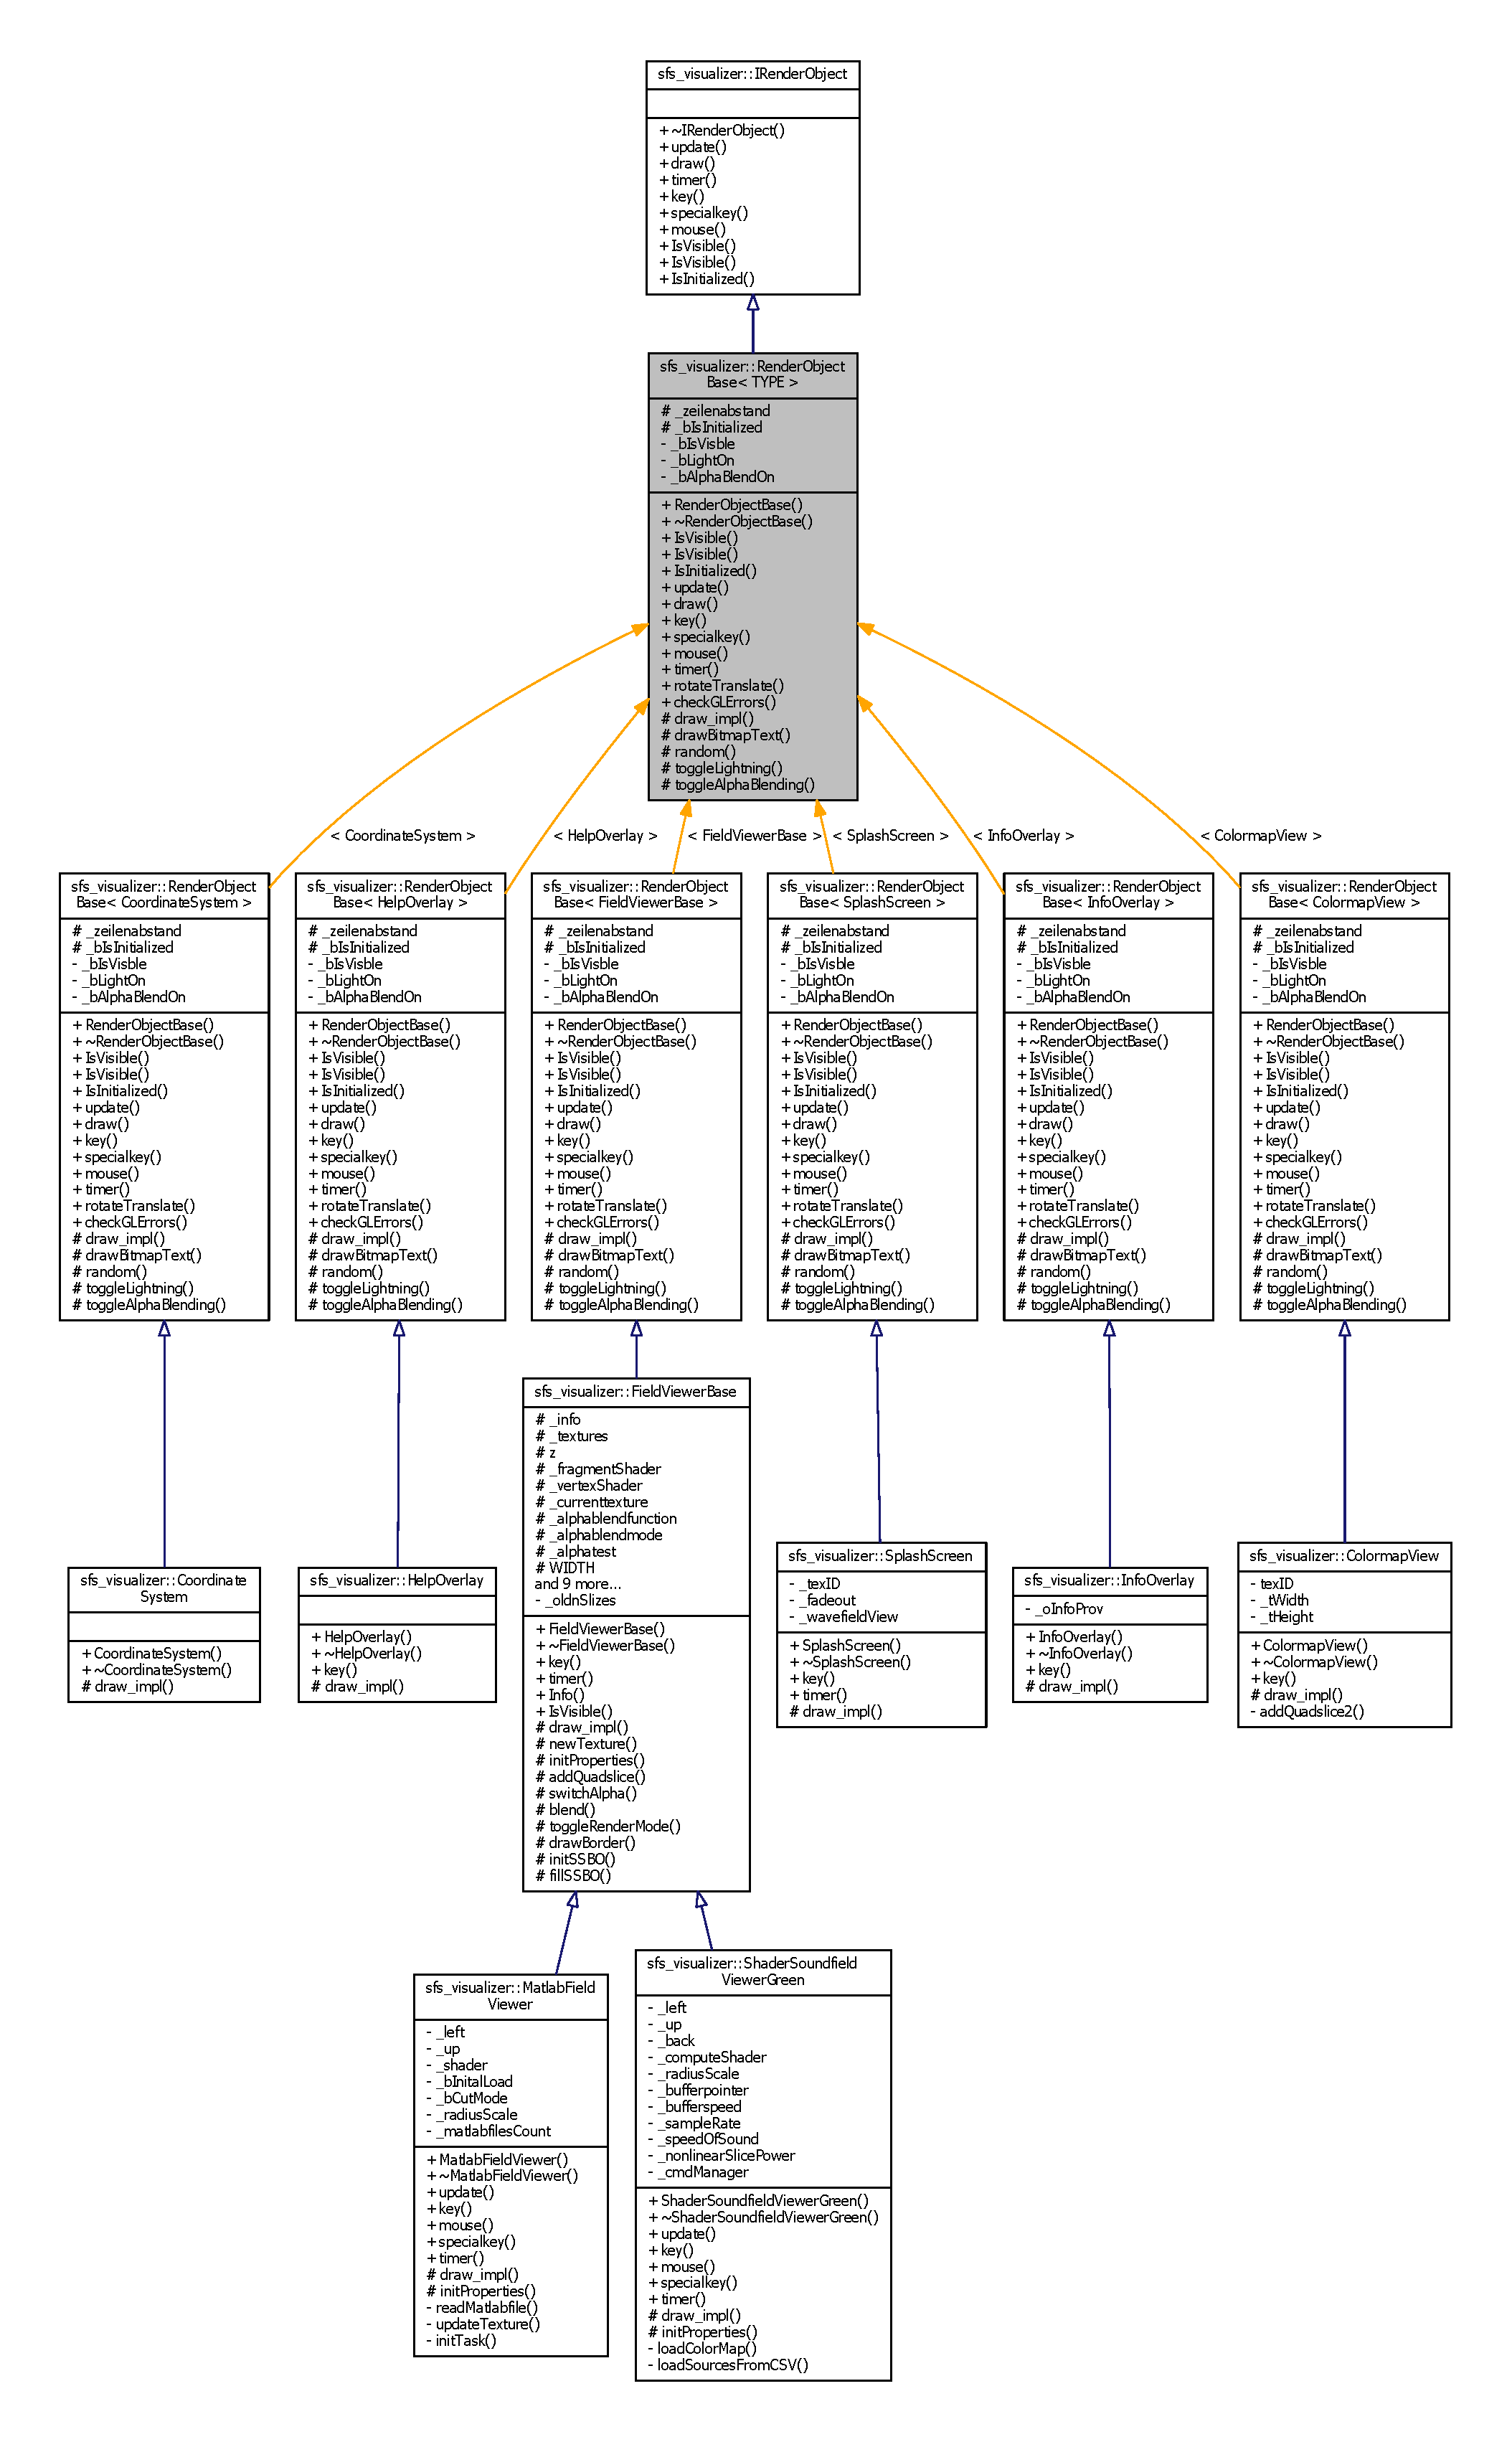
\includegraphics[height=550pt]{dc/de7/classsfs__visualizer_1_1RenderObjectBase__inherit__graph}
\end{center}
\end{figure}


Collaboration diagram for sfs\-\_\-visualizer\-:\-:Render\-Object\-Base$<$ T\-Y\-P\-E $>$\-:\nopagebreak
\begin{figure}[H]
\begin{center}
\leavevmode
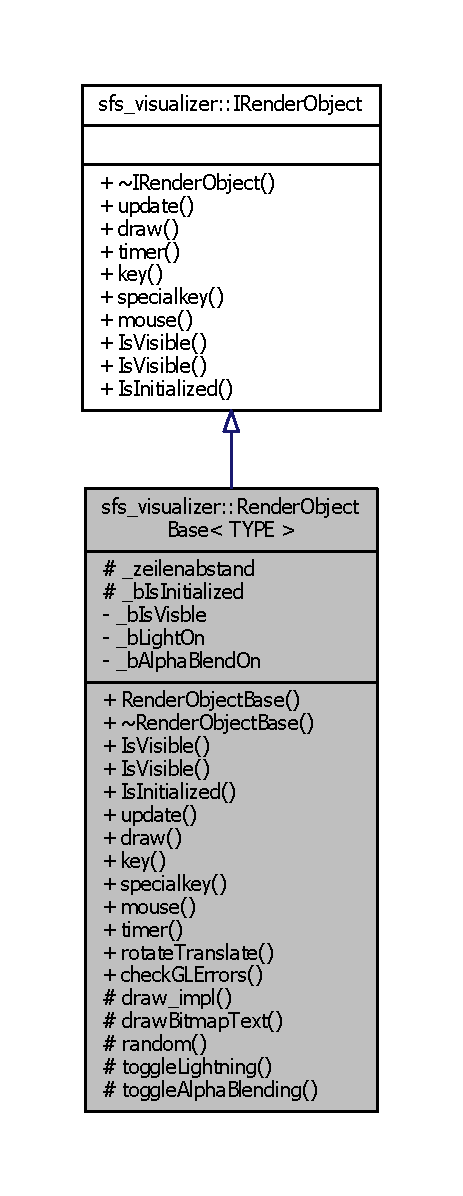
\includegraphics[height=550pt]{da/db7/classsfs__visualizer_1_1RenderObjectBase__coll__graph}
\end{center}
\end{figure}
\subsection*{Public Member Functions}
\begin{DoxyCompactItemize}
\item 
virtual bool {\bf Is\-Visible} ()
\begin{DoxyCompactList}\small\item\em mutators and informators \end{DoxyCompactList}\item 
virtual void {\bfseries Is\-Visible} (bool b\-Visible)\label{classsfs__visualizer_1_1RenderObjectBase_a2edc1e260fc6c838dadc26d5b6dce760}

\item 
virtual bool {\bfseries Is\-Initialized} ()\label{classsfs__visualizer_1_1RenderObjectBase_a4cf494c1fc7d41c0a734790cbd8a44c2}

\item 
virtual void {\bf update} ()
\begin{DoxyCompactList}\small\item\em methods \end{DoxyCompactList}\item 
virtual void {\bfseries draw} ()\label{classsfs__visualizer_1_1RenderObjectBase_a56f2b59b1546c94d2ac7553b3fee16e4}

\item 
virtual void {\bf key} (unsigned char key, int x, int y)
\begin{DoxyCompactList}\small\item\em user inputs \end{DoxyCompactList}\item 
virtual void {\bfseries specialkey} (int {\bf key}, int x, int y)\label{classsfs__visualizer_1_1RenderObjectBase_a483bbf988217483173e645c8acd42b75}

\item 
virtual void {\bfseries mouse} (int button, int state, int x, int y)\label{classsfs__visualizer_1_1RenderObjectBase_a093ef21415423a4fc8e69b64143ee7a3}

\item 
virtual void {\bfseries timer} (int update\-Rate\-Ms)\label{classsfs__visualizer_1_1RenderObjectBase_adfbc55cb448c161377b9086337a00c29}

\item 
virtual void {\bfseries rotate\-Translate} (float x\-Rot, float y\-Rot, float z\-Rot, float x\-Trans, float y\-Trans, float z\-Trans)\label{classsfs__visualizer_1_1RenderObjectBase_a75253def39e89b4114bcbfd91fab4428}

\end{DoxyCompactItemize}
\subsection*{Static Public Member Functions}
\begin{DoxyCompactItemize}
\item 
static bool {\bfseries check\-G\-L\-Errors} (const std\-::string \&info)\label{classsfs__visualizer_1_1RenderObjectBase_adfeee2bcdda8de4e318fd9897d50983e}

\end{DoxyCompactItemize}
\subsection*{Protected Member Functions}
\begin{DoxyCompactItemize}
\item 
virtual void {\bfseries draw\-\_\-impl} ()=0\label{classsfs__visualizer_1_1RenderObjectBase_a044990922855aba76b176c77f799beca}

\item 
void {\bfseries draw\-Bitmap\-Text} (const std\-::string \&str\-Value, float x, float y, float z)\label{classsfs__visualizer_1_1RenderObjectBase_a171675eae526d70ebb2efc61d7375165}

\item 
float {\bf random} ()
\begin{DoxyCompactList}\small\item\em Random float -\/0.\-5-\/0.\-5. \end{DoxyCompactList}\item 
void {\bfseries toggle\-Lightning} ()\label{classsfs__visualizer_1_1RenderObjectBase_a3d5f027a74cf05ef0bd06b63f586ff1f}

\item 
void {\bfseries toggle\-Alpha\-Blending} ()\label{classsfs__visualizer_1_1RenderObjectBase_a4be60990d3ae4f776ba98c8eb4c497c2}

\end{DoxyCompactItemize}
\subsection*{Protected Attributes}
\begin{DoxyCompactItemize}
\item 
float {\bfseries \-\_\-zeilenabstand}\label{classsfs__visualizer_1_1RenderObjectBase_a4113da2f216433932a31195d1c198c62}

\item 
bool {\bfseries \-\_\-b\-Is\-Initialized}\label{classsfs__visualizer_1_1RenderObjectBase_a77e847921c60f9da0413bde0257127b8}

\end{DoxyCompactItemize}
\subsection*{Private Attributes}
\begin{DoxyCompactItemize}
\item 
bool {\bfseries \-\_\-b\-Is\-Visble}\label{classsfs__visualizer_1_1RenderObjectBase_ab792bdd70a389d118529af2967d3ccec}

\item 
bool {\bfseries \-\_\-b\-Light\-On}\label{classsfs__visualizer_1_1RenderObjectBase_ae256f0c80ca08039842c95ccc25cb1f7}

\item 
bool {\bfseries \-\_\-b\-Alpha\-Blend\-On}\label{classsfs__visualizer_1_1RenderObjectBase_ab9e5ed07b9f54262a068da2dd5cb9cae}

\end{DoxyCompactItemize}


\subsection{Detailed Description}
\subsubsection*{template$<$class T\-Y\-P\-E$>$class sfs\-\_\-visualizer\-::\-Render\-Object\-Base$<$ T\-Y\-P\-E $>$}

Base for Render\-Objects, which are objects, that can be shown in 3\-D. 

Is used to share implementations for all Render\-Objects. 

Definition at line 26 of file renderobjectbase.\-h.



\subsection{Member Function Documentation}
\index{sfs\-\_\-visualizer\-::\-Render\-Object\-Base@{sfs\-\_\-visualizer\-::\-Render\-Object\-Base}!Is\-Visible@{Is\-Visible}}
\index{Is\-Visible@{Is\-Visible}!sfs_visualizer::RenderObjectBase@{sfs\-\_\-visualizer\-::\-Render\-Object\-Base}}
\subsubsection[{Is\-Visible}]{\setlength{\rightskip}{0pt plus 5cm}template$<$class T\-Y\-P\-E $>$ bool Render\-Object\-Base\-::\-Is\-Visible (
\begin{DoxyParamCaption}
{}
\end{DoxyParamCaption}
)\hspace{0.3cm}{\ttfamily [virtual]}}\label{classsfs__visualizer_1_1RenderObjectBase_a7bfad24bb32632b5328aa347faa3d129}


mutators and informators 



Implements {\bf sfs\-\_\-visualizer\-::\-I\-Render\-Object} \doxyref{}{p.}{da/d4f/classsfs__visualizer_1_1IRenderObject_a4160e34cad5f899a410650f2f979bb0d}.



Definition at line 76 of file renderobjectbase.\-h.



Referenced by sfs\-\_\-visualizer\-::\-Matlab\-Field\-Viewer\-::key().

\index{sfs\-\_\-visualizer\-::\-Render\-Object\-Base@{sfs\-\_\-visualizer\-::\-Render\-Object\-Base}!update@{update}}
\index{update@{update}!sfs_visualizer::RenderObjectBase@{sfs\-\_\-visualizer\-::\-Render\-Object\-Base}}
\subsubsection[{update}]{\setlength{\rightskip}{0pt plus 5cm}template$<$class T\-Y\-P\-E $>$ void Render\-Object\-Base\-::update (
\begin{DoxyParamCaption}
{}
\end{DoxyParamCaption}
)\hspace{0.3cm}{\ttfamily [virtual]}}\label{classsfs__visualizer_1_1RenderObjectBase_aab3270a6296d723574efcebe4d464ba9}


methods 



Implements {\bf sfs\-\_\-visualizer\-::\-I\-Render\-Object} \doxyref{}{p.}{da/d4f/classsfs__visualizer_1_1IRenderObject_addfa7be6b4cadc5e71d4bdcc8ef15fc7}.



Reimplemented in {\bf sfs\-\_\-visualizer\-::\-Shader\-Soundfield\-Viewer\-Green} \doxyref{}{p.}{d6/dab/classsfs__visualizer_1_1ShaderSoundfieldViewerGreen_a8acf805aa86680695d7ae1c380d214da}, and {\bf sfs\-\_\-visualizer\-::\-Matlab\-Field\-Viewer} \doxyref{}{p.}{d8/d1c/classsfs__visualizer_1_1MatlabFieldViewer_a4997514b7715c83d2c513576af0a2c60}.



Definition at line 110 of file renderobjectbase.\-h.

\index{sfs\-\_\-visualizer\-::\-Render\-Object\-Base@{sfs\-\_\-visualizer\-::\-Render\-Object\-Base}!key@{key}}
\index{key@{key}!sfs_visualizer::RenderObjectBase@{sfs\-\_\-visualizer\-::\-Render\-Object\-Base}}
\subsubsection[{key}]{\setlength{\rightskip}{0pt plus 5cm}template$<$class T\-Y\-P\-E $>$ void Render\-Object\-Base\-::key (
\begin{DoxyParamCaption}
\item[{unsigned char}]{key, }
\item[{int}]{x, }
\item[{int}]{y}
\end{DoxyParamCaption}
)\hspace{0.3cm}{\ttfamily [virtual]}}\label{classsfs__visualizer_1_1RenderObjectBase_a3f0106a0ce3861f34e5330da65e7bdd4}


user inputs 



Implements {\bf sfs\-\_\-visualizer\-::\-I\-Render\-Object} \doxyref{}{p.}{da/d4f/classsfs__visualizer_1_1IRenderObject_adee6c00f917851b6b96f6a88dbe4eb62}.



Reimplemented in {\bf sfs\-\_\-visualizer\-::\-Field\-Viewer\-Base} \doxyref{}{p.}{dc/dc0/classsfs__visualizer_1_1FieldViewerBase_acebb098dc25cd342be007c47cc2e64ab}, {\bf sfs\-\_\-visualizer\-::\-Shader\-Soundfield\-Viewer\-Green} \doxyref{}{p.}{d6/dab/classsfs__visualizer_1_1ShaderSoundfieldViewerGreen_a5a2363722318f189a5c5276d64659776}, {\bf sfs\-\_\-visualizer\-::\-Matlab\-Field\-Viewer} \doxyref{}{p.}{d8/d1c/classsfs__visualizer_1_1MatlabFieldViewer_aaba2a2a82434165851e44a01f299d58b}, {\bf sfs\-\_\-visualizer\-::\-Info\-Overlay} \doxyref{}{p.}{d7/d78/classsfs__visualizer_1_1InfoOverlay_ad04dcece97043b948ae9af471172e5c0}, {\bf sfs\-\_\-visualizer\-::\-Colormap\-View} \doxyref{}{p.}{de/dbd/classsfs__visualizer_1_1ColormapView_af9381d745eb32e41fbc588cb325ffe4c}, {\bf sfs\-\_\-visualizer\-::\-Help\-Overlay} \doxyref{}{p.}{d4/db2/classsfs__visualizer_1_1HelpOverlay_af073d80d01dc30a14a40238b9d539d14}, and {\bf sfs\-\_\-visualizer\-::\-Splash\-Screen} \doxyref{}{p.}{df/d2f/classsfs__visualizer_1_1SplashScreen_abc2cf866fa07a5bc66271622d12c8d6a}.



Definition at line 94 of file renderobjectbase.\-h.

\index{sfs\-\_\-visualizer\-::\-Render\-Object\-Base@{sfs\-\_\-visualizer\-::\-Render\-Object\-Base}!random@{random}}
\index{random@{random}!sfs_visualizer::RenderObjectBase@{sfs\-\_\-visualizer\-::\-Render\-Object\-Base}}
\subsubsection[{random}]{\setlength{\rightskip}{0pt plus 5cm}template$<$class T\-Y\-P\-E $>$ float Render\-Object\-Base\-::random (
\begin{DoxyParamCaption}
{}
\end{DoxyParamCaption}
)\hspace{0.3cm}{\ttfamily [protected]}}\label{classsfs__visualizer_1_1RenderObjectBase_a5611a9ea412e0bf33eeeb3aab5a2a097}


Random float -\/0.\-5-\/0.\-5. 



Definition at line 197 of file renderobjectbase.\-h.



The documentation for this class was generated from the following file\-:\begin{DoxyCompactItemize}
\item 
renderobjectbase.\-h\end{DoxyCompactItemize}

\section{Render\-Object\-Base Class Reference}
\label{classRenderObjectBase}\index{Render\-Object\-Base@{Render\-Object\-Base}}


{\ttfamily \#include $<$renderobjectbase.\-h$>$}



Collaboration diagram for Render\-Object\-Base\-:
\nopagebreak
\begin{figure}[H]
\begin{center}
\leavevmode
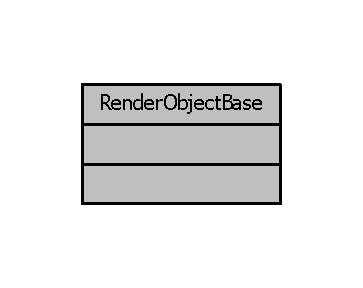
\includegraphics[width=174pt]{d4/d2e/classRenderObjectBase__coll__graph}
\end{center}
\end{figure}


\subsection{Detailed Description}
\begin{DoxyAuthor}{Author}
Marcus Zepp
\end{DoxyAuthor}
\begin{DoxyVersion}{Version}

\end{DoxyVersion}
\begin{DoxyParagraph}{Revision\-:}
1.\-0 
\end{DoxyParagraph}


\begin{DoxyDate}{Date}

\end{DoxyDate}
\begin{DoxyParagraph}{Date\-:}
2014/03/26 14\-:16\-:20 
\end{DoxyParagraph}


Contact\-: {\tt zeppfisj@mailbox.\-tu-\/berlin.\-de} 

The documentation for this class was generated from the following file\-:\begin{DoxyCompactItemize}
\item 
renderobjectbase.\-h\end{DoxyCompactItemize}

\section{Shader Class Reference}
\label{classShader}\index{Shader@{Shader}}


{\ttfamily \#include $<$shader.\-h$>$}



Collaboration diagram for Shader\-:
\nopagebreak
\begin{figure}[H]
\begin{center}
\leavevmode
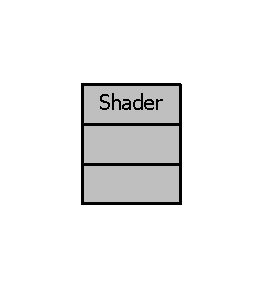
\includegraphics[width=126pt]{d9/dba/classShader__coll__graph}
\end{center}
\end{figure}


\subsection{Detailed Description}
\begin{DoxyAuthor}{Author}
Marcus Zepp
\end{DoxyAuthor}
\begin{DoxyVersion}{Version}

\end{DoxyVersion}
\begin{DoxyParagraph}{Revision\-:}
1.\-0 
\end{DoxyParagraph}


\begin{DoxyDate}{Date}

\end{DoxyDate}
\begin{DoxyParagraph}{Date\-:}
2014/03/26 14\-:16\-:20 
\end{DoxyParagraph}


Contact\-: {\tt zeppfisj@mailbox.\-tu-\/berlin.\-de} 

The documentation for this class was generated from the following file\-:\begin{DoxyCompactItemize}
\item 
shader.\-h\end{DoxyCompactItemize}

\section{sfs\-\_\-visualizer\-:\-:Shader Class Reference}
\label{classsfs__visualizer_1_1Shader}\index{sfs\-\_\-visualizer\-::\-Shader@{sfs\-\_\-visualizer\-::\-Shader}}


class to load glsl-\/shaders and wraps communication with uniform-\/values, that are the variables of shaders  




{\ttfamily \#include $<$shader.\-h$>$}



Collaboration diagram for sfs\-\_\-visualizer\-:\-:Shader\-:\nopagebreak
\begin{figure}[H]
\begin{center}
\leavevmode
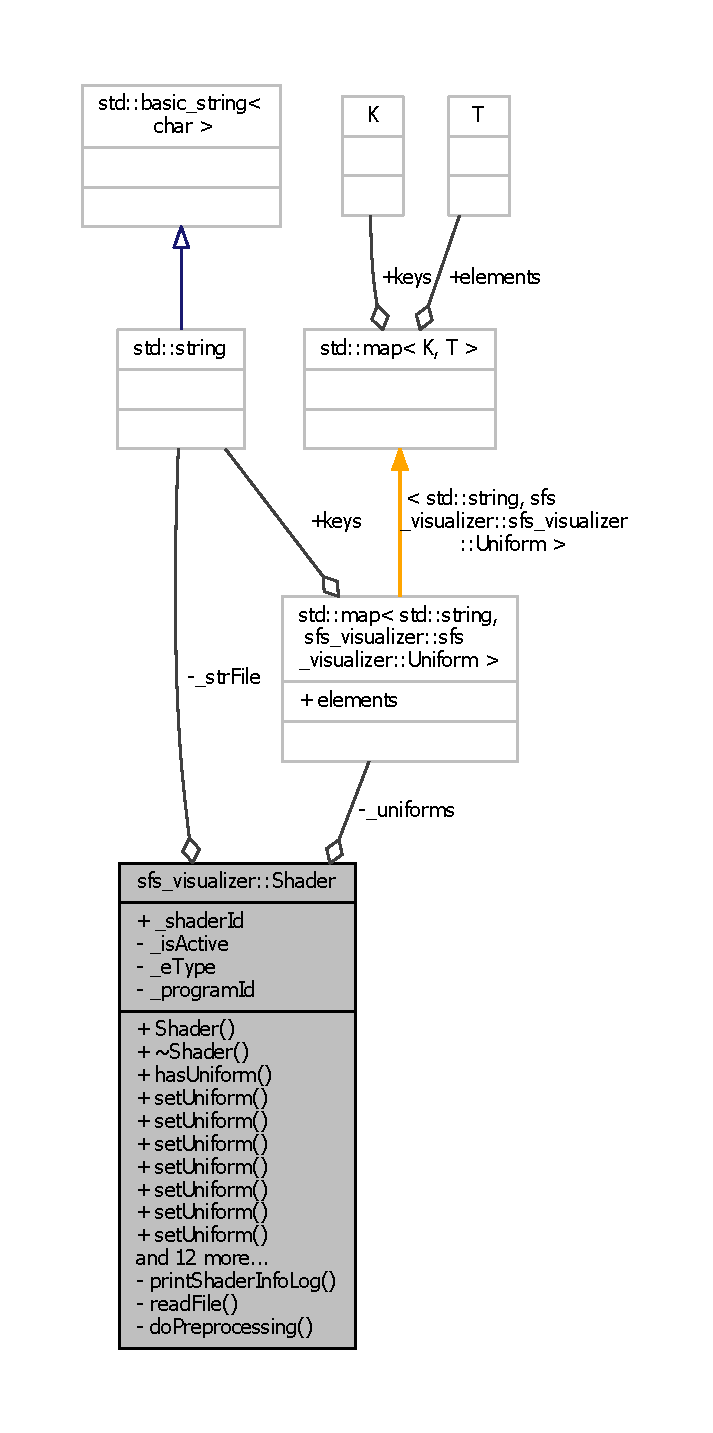
\includegraphics[height=550pt]{d2/d83/classsfs__visualizer_1_1Shader__coll__graph}
\end{center}
\end{figure}
\subsection*{Public Member Functions}
\begin{DoxyCompactItemize}
\item 
{\bfseries Shader} (std\-::string str\-File, Shader\-Type type)\label{classsfs__visualizer_1_1Shader_a788625a07b6ab1a9289f7908d57fbcee}

\item 
bool {\bfseries has\-Uniform} (const std\-::string \&name)\label{classsfs__visualizer_1_1Shader_aafd1573a18131732760d145980faa29b}

\item 
void {\bfseries set\-Uniform} (const std\-::string \&name, int v1)\label{classsfs__visualizer_1_1Shader_a7c338cb2207bf8f07f01e660e66fd074}

\item 
void {\bfseries set\-Uniform} (const std\-::string \&name, unsigned int v1)\label{classsfs__visualizer_1_1Shader_a765c976862f1b7b195753203d809ee81}

\item 
void {\bfseries set\-Uniform} (const std\-::string \&name, float v1)\label{classsfs__visualizer_1_1Shader_a4a3b23dc158f7b807637d7bfe45e06df}

\item 
void {\bfseries set\-Uniform} (const std\-::string \&name, float v1, float v2)\label{classsfs__visualizer_1_1Shader_a49421168f8dde7eceb27a3b81476f9a8}

\item 
void {\bfseries set\-Uniform} (const std\-::string \&name, float v1, float v2, float v3)\label{classsfs__visualizer_1_1Shader_a28860ee636ca9be63aa01b1d26af8c73}

\item 
void {\bfseries set\-Uniform} (const std\-::string \&name, float v1, float v2, float v3, float v4)\label{classsfs__visualizer_1_1Shader_a1c5a47ed1c0b4c717a2c814ae11c1aba}

\item 
void {\bfseries set\-Uniform} (const std\-::string \&name, int count, float $\ast$v1)\label{classsfs__visualizer_1_1Shader_a86a3b0dd818a86e00ce4f65ed6f60155}

\item 
void {\bfseries set\-Uniform\-Array} (const std\-::string \&name, int count, float $\ast$v1)\label{classsfs__visualizer_1_1Shader_a7e9a6db4e87a10c28b54629beff7134a}

\item 
void {\bfseries set\-Uniform\-Vec4\-Array} (const std\-::string \&name, int count, float $\ast$v1)\label{classsfs__visualizer_1_1Shader_a66d2819b9cc558dbcedf1cd45c0e4cbd}

\item 
void {\bfseries set\-Uniform\-Array} (const std\-::string \&name, int count, unsigned int $\ast$v1)\label{classsfs__visualizer_1_1Shader_a4144a18c538d3bfc348d358a3a7e949a}

\item 
void {\bfseries set\-Uniform\-Matrix} (const std\-::string \&name, int count, float $\ast$v1)\label{classsfs__visualizer_1_1Shader_a4ac702af346f3cf8e14998bb4f59e326}

\item 
void {\bfseries update\-Uniforms} ()\label{classsfs__visualizer_1_1Shader_a605b87e078f7eaf0cf9777f7f6319311}

\item 
void {\bfseries load} ()\label{classsfs__visualizer_1_1Shader_a4222b925de192c794cdef621b13a5914}

\item 
void {\bfseries un\-Load} ()\label{classsfs__visualizer_1_1Shader_aa6e66aded6c712272998a146372850b0}

\item 
void {\bfseries attach\-Shader} (G\-Luint shader\-\_\-id)\label{classsfs__visualizer_1_1Shader_a0d5dc86ead4edde7010b76cb7df2ec46}

\item 
void {\bfseries create\-Program} ()\label{classsfs__visualizer_1_1Shader_ab3ceeba9cf9f760fc3eaa97e81578103}

\item 
void {\bfseries link\-Program} ()\label{classsfs__visualizer_1_1Shader_a75c069ae57bc198b229bd56b18e9b459}

\item 
void {\bfseries use} ()\label{classsfs__visualizer_1_1Shader_a870fa9f13d69e558815d6fd351a469dc}

\item 
bool {\bfseries is\-Active} ()\label{classsfs__visualizer_1_1Shader_a89103f6e4224e366307b7a89898f2a0f}

\end{DoxyCompactItemize}
\subsection*{Public Attributes}
\begin{DoxyCompactItemize}
\item 
G\-Luint {\bfseries \-\_\-shader\-Id}\label{classsfs__visualizer_1_1Shader_aed41f9ecc4dcc30ee1d307d33b48cd21}

\end{DoxyCompactItemize}
\subsection*{Private Member Functions}
\begin{DoxyCompactItemize}
\item 
void {\bfseries print\-Shader\-Info\-Log} (G\-Luint obj)\label{classsfs__visualizer_1_1Shader_a9c337c0dfcaf6a71ac6af7f6e75491eb}

\item 
std\-::string {\bfseries read\-File} (const std\-::string \&str\-File\-Name)\label{classsfs__visualizer_1_1Shader_a492073213e8668a330a327cee21f9418}

\item 
void {\bfseries do\-Preprocessing} (std\-::string \&str\-Text)\label{classsfs__visualizer_1_1Shader_ac122180bc89600c2932a7a65e805815e}

\end{DoxyCompactItemize}
\subsection*{Private Attributes}
\begin{DoxyCompactItemize}
\item 
bool {\bfseries \-\_\-is\-Active}\label{classsfs__visualizer_1_1Shader_ac22f274abcb33588ad9e1815a960f33c}

\item 
std\-::string {\bfseries \-\_\-str\-File}\label{classsfs__visualizer_1_1Shader_af8fd08acce17bfc88b0cfe9136c982ca}

\item 
Shader\-Type {\bfseries \-\_\-e\-Type}\label{classsfs__visualizer_1_1Shader_af546a04c628927c44edb9d088149433e}

\item 
std\-::map$<$ std\-::string, \\*
{\bf sfs\-\_\-visualizer\-::\-Uniform} $>$ {\bfseries \-\_\-uniforms}\label{classsfs__visualizer_1_1Shader_a849d6a90553c7f1d556414d965e12444}

\item 
G\-Luint {\bfseries \-\_\-program\-Id}\label{classsfs__visualizer_1_1Shader_a000cea3767f7e0357c04da5b94fa9b61}

\end{DoxyCompactItemize}


\subsection{Detailed Description}
class to load glsl-\/shaders and wraps communication with uniform-\/values, that are the variables of shaders 

Definition at line 52 of file shader.\-h.



The documentation for this class was generated from the following files\-:\begin{DoxyCompactItemize}
\item 
shader.\-h\item 
shader.\-cpp\end{DoxyCompactItemize}

\section{Sound\-Field\-Viewer\-:\-:Shader\-Loader Class Reference}
\label{classSoundFieldViewer_1_1ShaderLoader}\index{Sound\-Field\-Viewer\-::\-Shader\-Loader@{Sound\-Field\-Viewer\-::\-Shader\-Loader}}


Collaboration diagram for Sound\-Field\-Viewer\-:\-:Shader\-Loader\-:
\nopagebreak
\begin{figure}[H]
\begin{center}
\leavevmode
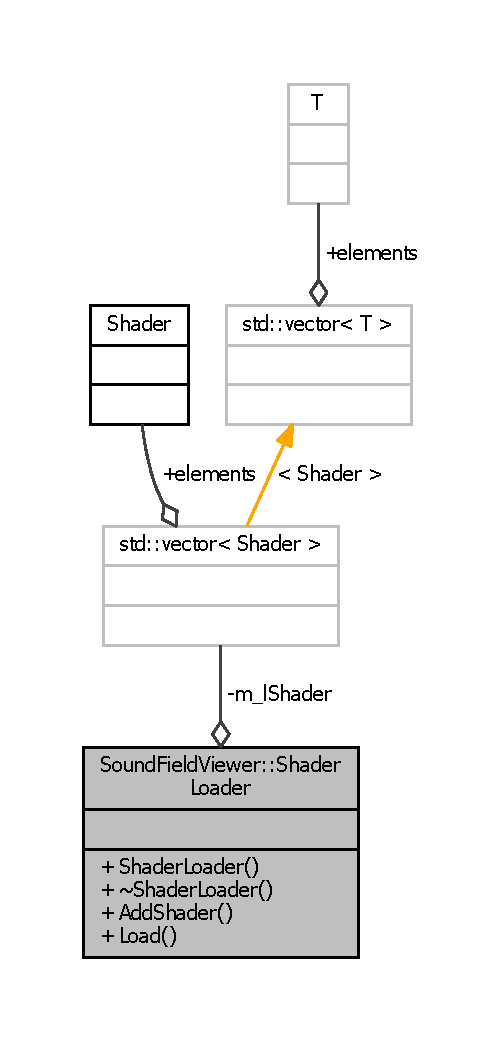
\includegraphics[width=242pt]{dc/dd8/classSoundFieldViewer_1_1ShaderLoader__coll__graph}
\end{center}
\end{figure}
\subsection*{Public Member Functions}
\begin{DoxyCompactItemize}
\item 
void {\bfseries Add\-Shader} (std\-::string str\-File, Shader\-Type type)\label{classSoundFieldViewer_1_1ShaderLoader_a5342c3734c9bb71c5d7bd00fddf79772}

\item 
void {\bfseries Load} ()\label{classSoundFieldViewer_1_1ShaderLoader_a5dc4bc1ade5005d7ee17247feb9bcb91}

\end{DoxyCompactItemize}
\subsection*{Private Attributes}
\begin{DoxyCompactItemize}
\item 
std\-::vector$<$ {\bf Shader} $>$ {\bfseries m\-\_\-l\-Shader}\label{classSoundFieldViewer_1_1ShaderLoader_ad755652c68508c858d8d4972dbadbaa3}

\end{DoxyCompactItemize}


\subsection{Detailed Description}


Definition at line 9 of file shaderloader.\-h.



The documentation for this class was generated from the following files\-:\begin{DoxyCompactItemize}
\item 
shaderloader.\-h\item 
shaderloader.\-cpp\end{DoxyCompactItemize}

\section{sfs\-\_\-visualizer\-:\-:Shader\-Soundfield\-Viewer\-Green Class Reference}
\label{classsfs__visualizer_1_1ShaderSoundfieldViewerGreen}\index{sfs\-\_\-visualizer\-::\-Shader\-Soundfield\-Viewer\-Green@{sfs\-\_\-visualizer\-::\-Shader\-Soundfield\-Viewer\-Green}}


A Field\-Viewer that loads a compute shader to compute W\-F\-S.  




{\ttfamily \#include $<$shadersoundfieldviewergreen.\-h$>$}



Inheritance diagram for sfs\-\_\-visualizer\-:\-:Shader\-Soundfield\-Viewer\-Green\-:
\nopagebreak
\begin{figure}[H]
\begin{center}
\leavevmode
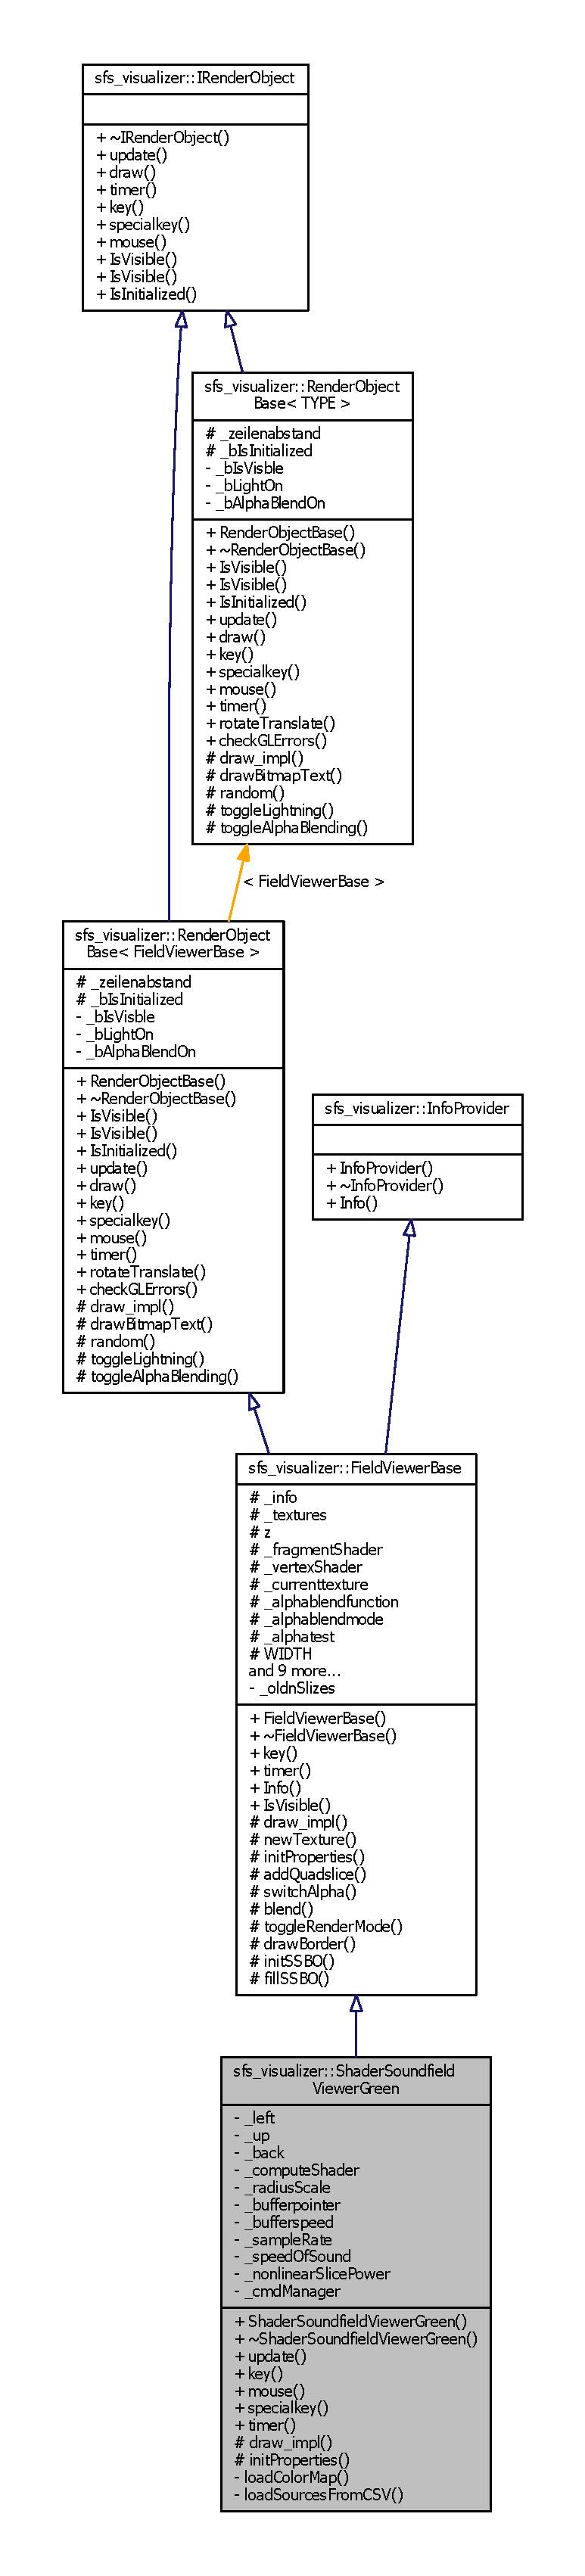
\includegraphics[height=550pt]{db/d54/classsfs__visualizer_1_1ShaderSoundfieldViewerGreen__inherit__graph}
\end{center}
\end{figure}


Collaboration diagram for sfs\-\_\-visualizer\-:\-:Shader\-Soundfield\-Viewer\-Green\-:
\nopagebreak
\begin{figure}[H]
\begin{center}
\leavevmode
\includegraphics[height=550pt]{d6/d11/classsfs__visualizer_1_1ShaderSoundfieldViewerGreen__coll__graph}
\end{center}
\end{figure}
\subsection*{Public Member Functions}
\begin{DoxyCompactItemize}
\item 
virtual void {\bf update} ()
\begin{DoxyCompactList}\small\item\em methods \end{DoxyCompactList}\item 
virtual void {\bf key} (unsigned char key, int x, int y)
\begin{DoxyCompactList}\small\item\em user inputs \end{DoxyCompactList}\item 
virtual void {\bfseries mouse} (int button, int state, int x, int y)\label{classsfs__visualizer_1_1ShaderSoundfieldViewerGreen_a893d9adbab65d3f907771f1a3f39aaf8}

\item 
virtual void {\bfseries specialkey} (int {\bf key}, int x, int y)\label{classsfs__visualizer_1_1ShaderSoundfieldViewerGreen_a7fd528f8597fe83b8468ce769457be65}

\item 
virtual void {\bfseries timer} (int update\-Rate\-Ms)\label{classsfs__visualizer_1_1ShaderSoundfieldViewerGreen_aa3134dfa4af254be92e25a812dba6700}

\end{DoxyCompactItemize}
\subsection*{Protected Member Functions}
\begin{DoxyCompactItemize}
\item 
virtual void {\bfseries draw\-\_\-impl} ()\label{classsfs__visualizer_1_1ShaderSoundfieldViewerGreen_a2c94ec45898febade515dd2f4731166a}

\item 
virtual void {\bfseries init\-Properties} ()\label{classsfs__visualizer_1_1ShaderSoundfieldViewerGreen_af8719f79560e7b99bc49a68d9664357b}

\end{DoxyCompactItemize}
\subsection*{Private Member Functions}
\begin{DoxyCompactItemize}
\item 
void {\bfseries load\-Color\-Map} ()\label{classsfs__visualizer_1_1ShaderSoundfieldViewerGreen_a5178491b6c94594e6eb9021e6fe876a2}

\item 
void {\bfseries load\-Sources\-From\-C\-S\-V} ()\label{classsfs__visualizer_1_1ShaderSoundfieldViewerGreen_a52eb625785193f29dc1f418d1826715f}

\end{DoxyCompactItemize}
\subsection*{Private Attributes}
\begin{DoxyCompactItemize}
\item 
float {\bfseries \-\_\-left}\label{classsfs__visualizer_1_1ShaderSoundfieldViewerGreen_a96dae44fa8beac7ebc4a8e7bda8113b2}

\item 
float {\bfseries \-\_\-up}\label{classsfs__visualizer_1_1ShaderSoundfieldViewerGreen_a08a415d59e222d09ae17aa253a2e4813}

\item 
float {\bfseries \-\_\-back}\label{classsfs__visualizer_1_1ShaderSoundfieldViewerGreen_a9f0551f9b02131c506c0feded41a4f91}

\item 
{\bf Shader} $\ast$ {\bfseries \-\_\-compute\-Shader}\label{classsfs__visualizer_1_1ShaderSoundfieldViewerGreen_a5245cbb5fcbb71dc4f257dd9bcfaba58}

\item 
float {\bfseries \-\_\-radius\-Scale}\label{classsfs__visualizer_1_1ShaderSoundfieldViewerGreen_a45f4decd211eff14418c40db2dec042b}

\item 
float {\bfseries \-\_\-bufferpointer}\label{classsfs__visualizer_1_1ShaderSoundfieldViewerGreen_a79c862245853b08e7a5a420a9837a8a9}

\item 
float {\bfseries \-\_\-bufferspeed}\label{classsfs__visualizer_1_1ShaderSoundfieldViewerGreen_a4133894835336d6e79d9150e427538d5}

\item 
float {\bfseries \-\_\-sample\-Rate}\label{classsfs__visualizer_1_1ShaderSoundfieldViewerGreen_a681f93b842e79dd271ebcf69130866e3}

\item 
float {\bfseries \-\_\-speed\-Of\-Sound}\label{classsfs__visualizer_1_1ShaderSoundfieldViewerGreen_ad148a9857df85ab01c937b4f16fe24fe}

\item 
float {\bfseries \-\_\-nonlinear\-Slice\-Power}\label{classsfs__visualizer_1_1ShaderSoundfieldViewerGreen_a63babad5b7f11b9aa189859e4771f19c}

\item 
{\bf Command\-Manager} {\bfseries \-\_\-cmd\-Manager}\label{classsfs__visualizer_1_1ShaderSoundfieldViewerGreen_a4471696bf41bc8f0118a597ea117ff3c}

\end{DoxyCompactItemize}
\subsection*{Additional Inherited Members}


\subsection{Detailed Description}
A Field\-Viewer that loads a compute shader to compute W\-F\-S. 

Definition at line 30 of file shadersoundfieldviewergreen.\-h.



\subsection{Member Function Documentation}
\index{sfs\-\_\-visualizer\-::\-Shader\-Soundfield\-Viewer\-Green@{sfs\-\_\-visualizer\-::\-Shader\-Soundfield\-Viewer\-Green}!update@{update}}
\index{update@{update}!sfs_visualizer::ShaderSoundfieldViewerGreen@{sfs\-\_\-visualizer\-::\-Shader\-Soundfield\-Viewer\-Green}}
\subsubsection[{update}]{\setlength{\rightskip}{0pt plus 5cm}void Shader\-Soundfield\-Viewer\-Green\-::update (
\begin{DoxyParamCaption}
{}
\end{DoxyParamCaption}
)\hspace{0.3cm}{\ttfamily [virtual]}}\label{classsfs__visualizer_1_1ShaderSoundfieldViewerGreen_a8acf805aa86680695d7ae1c380d214da}


methods 



Reimplemented from {\bf sfs\-\_\-visualizer\-::\-Render\-Object\-Base$<$ Field\-Viewer\-Base $>$} \doxyref{}{p.}{de/d2a/classsfs__visualizer_1_1RenderObjectBase_aab3270a6296d723574efcebe4d464ba9}.



Definition at line 304 of file shadersoundfieldviewergreen.\-cpp.

\index{sfs\-\_\-visualizer\-::\-Shader\-Soundfield\-Viewer\-Green@{sfs\-\_\-visualizer\-::\-Shader\-Soundfield\-Viewer\-Green}!key@{key}}
\index{key@{key}!sfs_visualizer::ShaderSoundfieldViewerGreen@{sfs\-\_\-visualizer\-::\-Shader\-Soundfield\-Viewer\-Green}}
\subsubsection[{key}]{\setlength{\rightskip}{0pt plus 5cm}void Shader\-Soundfield\-Viewer\-Green\-::key (
\begin{DoxyParamCaption}
\item[{unsigned char}]{key, }
\item[{int}]{x, }
\item[{int}]{y}
\end{DoxyParamCaption}
)\hspace{0.3cm}{\ttfamily [virtual]}}\label{classsfs__visualizer_1_1ShaderSoundfieldViewerGreen_a5a2363722318f189a5c5276d64659776}


user inputs 



Reimplemented from {\bf sfs\-\_\-visualizer\-::\-Field\-Viewer\-Base} \doxyref{}{p.}{dc/dc0/classsfs__visualizer_1_1FieldViewerBase_acebb098dc25cd342be007c47cc2e64ab}.



Definition at line 189 of file shadersoundfieldviewergreen.\-cpp.



The documentation for this class was generated from the following files\-:\begin{DoxyCompactItemize}
\item 
shadersoundfieldviewergreen.\-h\item 
shadersoundfieldviewergreen.\-cpp\end{DoxyCompactItemize}

\section{Shader\-Soundfield\-Viewer\-Green Class Reference}
\label{classShaderSoundfieldViewerGreen}\index{Shader\-Soundfield\-Viewer\-Green@{Shader\-Soundfield\-Viewer\-Green}}


{\ttfamily \#include $<$shadersoundfieldviewergreen.\-h$>$}



Collaboration diagram for Shader\-Soundfield\-Viewer\-Green\-:
\nopagebreak
\begin{figure}[H]
\begin{center}
\leavevmode
\includegraphics[width=228pt]{d1/d56/classShaderSoundfieldViewerGreen__coll__graph}
\end{center}
\end{figure}


\subsection{Detailed Description}
\begin{DoxyAuthor}{Author}
Marcus Zepp
\end{DoxyAuthor}
\begin{DoxyVersion}{Version}

\end{DoxyVersion}
\begin{DoxyParagraph}{Revision\-:}
1.\-0 
\end{DoxyParagraph}


\begin{DoxyDate}{Date}

\end{DoxyDate}
\begin{DoxyParagraph}{Date\-:}
2014/03/26 14\-:16\-:20 
\end{DoxyParagraph}


Contact\-: {\tt zeppfisj@mailbox.\-tu-\/berlin.\-de} 

The documentation for this class was generated from the following file\-:\begin{DoxyCompactItemize}
\item 
shadersoundfieldviewergreen.\-h\end{DoxyCompactItemize}

\section{Splash\-Screen Class Reference}
\label{classSplashScreen}\index{Splash\-Screen@{Splash\-Screen}}


{\ttfamily \#include $<$splashscreen.\-h$>$}



Collaboration diagram for Splash\-Screen\-:
\nopagebreak
\begin{figure}[H]
\begin{center}
\leavevmode
\includegraphics[width=154pt]{df/d98/classSplashScreen__coll__graph}
\end{center}
\end{figure}


\subsection{Detailed Description}
\begin{DoxyAuthor}{Author}
Marcus Zepp
\end{DoxyAuthor}
\begin{DoxyVersion}{Version}

\end{DoxyVersion}
\begin{DoxyParagraph}{Revision\-:}
1.\-0 
\end{DoxyParagraph}


\begin{DoxyDate}{Date}

\end{DoxyDate}
\begin{DoxyParagraph}{Date\-:}
2014/03/26 14\-:16\-:20 
\end{DoxyParagraph}


Contact\-: {\tt zeppfisj@mailbox.\-tu-\/berlin.\-de} 

The documentation for this class was generated from the following file\-:\begin{DoxyCompactItemize}
\item 
splashscreen.\-h\end{DoxyCompactItemize}

\section{sfs\-\_\-visualizer\-:\-:Splash\-Screen Class Reference}
\label{classsfs__visualizer_1_1SplashScreen}\index{sfs\-\_\-visualizer\-::\-Splash\-Screen@{sfs\-\_\-visualizer\-::\-Splash\-Screen}}


A Render\-Object, that displays the splashcreen at startup.  




{\ttfamily \#include $<$splashscreen.\-h$>$}



Inheritance diagram for sfs\-\_\-visualizer\-:\-:Splash\-Screen\-:\nopagebreak
\begin{figure}[H]
\begin{center}
\leavevmode
\includegraphics[height=550pt]{d7/d89/classsfs__visualizer_1_1SplashScreen__inherit__graph}
\end{center}
\end{figure}


Collaboration diagram for sfs\-\_\-visualizer\-:\-:Splash\-Screen\-:\nopagebreak
\begin{figure}[H]
\begin{center}
\leavevmode
\includegraphics[height=550pt]{d5/d97/classsfs__visualizer_1_1SplashScreen__coll__graph}
\end{center}
\end{figure}
\subsection*{Public Member Functions}
\begin{DoxyCompactItemize}
\item 
{\bfseries Splash\-Screen} ({\bf I\-Render\-Object} $\ast$wavefield\-View)\label{classsfs__visualizer_1_1SplashScreen_ad06a6b817747c4a56b34028d007c3d47}

\item 
virtual void {\bf key} (unsigned char key, int x, int y)
\begin{DoxyCompactList}\small\item\em user inputs \end{DoxyCompactList}\item 
virtual void {\bfseries timer} (int update\-Rate\-Ms)\label{classsfs__visualizer_1_1SplashScreen_ae8bd4570391caa94c542fb987280748c}

\end{DoxyCompactItemize}
\subsection*{Protected Member Functions}
\begin{DoxyCompactItemize}
\item 
virtual void {\bfseries draw\-\_\-impl} ()\label{classsfs__visualizer_1_1SplashScreen_a78bba58ad3d9dc26fcaaa58191273c34}

\end{DoxyCompactItemize}
\subsection*{Private Attributes}
\begin{DoxyCompactItemize}
\item 
int {\bfseries \-\_\-tex\-I\-D}\label{classsfs__visualizer_1_1SplashScreen_accccfff1033247252eb633374c9e2543}

\item 
float {\bfseries \-\_\-fadeout}\label{classsfs__visualizer_1_1SplashScreen_a55fccb7bfd315296ca2a5f1fecc4aeb3}

\item 
{\bf I\-Render\-Object} $\ast$ {\bfseries \-\_\-wavefield\-View}\label{classsfs__visualizer_1_1SplashScreen_a1b27283f8edd7c17543200c59771103e}

\end{DoxyCompactItemize}
\subsection*{Additional Inherited Members}


\subsection{Detailed Description}
A Render\-Object, that displays the splashcreen at startup. 

Definition at line 24 of file splashscreen.\-h.



\subsection{Member Function Documentation}
\index{sfs\-\_\-visualizer\-::\-Splash\-Screen@{sfs\-\_\-visualizer\-::\-Splash\-Screen}!key@{key}}
\index{key@{key}!sfs_visualizer::SplashScreen@{sfs\-\_\-visualizer\-::\-Splash\-Screen}}
\subsubsection[{key}]{\setlength{\rightskip}{0pt plus 5cm}void Splash\-Screen\-::key (
\begin{DoxyParamCaption}
\item[{unsigned char}]{key, }
\item[{int}]{x, }
\item[{int}]{y}
\end{DoxyParamCaption}
)\hspace{0.3cm}{\ttfamily [virtual]}}\label{classsfs__visualizer_1_1SplashScreen_abc2cf866fa07a5bc66271622d12c8d6a}


user inputs 



Reimplemented from {\bf sfs\-\_\-visualizer\-::\-Render\-Object\-Base$<$ Splash\-Screen $>$} \doxyref{}{p.}{de/d2a/classsfs__visualizer_1_1RenderObjectBase_a3f0106a0ce3861f34e5330da65e7bdd4}.



Definition at line 32 of file splashscreen.\-cpp.



References sfs\-\_\-visualizer\-::\-Render\-Object\-Base$<$ Splash\-Screen $>$\-::\-Is\-Visible().



The documentation for this class was generated from the following files\-:\begin{DoxyCompactItemize}
\item 
splashscreen.\-h\item 
splashscreen.\-cpp\end{DoxyCompactItemize}

\section{sfs\-\_\-visualizer\-:\-:Statistics Struct Reference}
\label{structsfs__visualizer_1_1Statistics}\index{sfs\-\_\-visualizer\-::\-Statistics@{sfs\-\_\-visualizer\-::\-Statistics}}


struct to keep statistical data  




{\ttfamily \#include $<$texturefactory.\-h$>$}



Collaboration diagram for sfs\-\_\-visualizer\-:\-:Statistics\-:
\nopagebreak
\begin{figure}[H]
\begin{center}
\leavevmode
\includegraphics[width=198pt]{d5/d69/structsfs__visualizer_1_1Statistics__coll__graph}
\end{center}
\end{figure}
\subsection*{Public Attributes}
\begin{DoxyCompactItemize}
\item 
float {\bfseries max\-R}\label{structsfs__visualizer_1_1Statistics_a92ab59196a4b4dce32eb9ef1a1b5f8be}

\item 
float {\bfseries max\-G}\label{structsfs__visualizer_1_1Statistics_a69ca010556d08541a3f8ce32250ec82c}

\item 
float {\bfseries max\-B}\label{structsfs__visualizer_1_1Statistics_ab8e57595c683f335b377e23a21fe8228}

\item 
float {\bfseries max\-A}\label{structsfs__visualizer_1_1Statistics_a1ec679a0f8d010f4068645a7797cccb6}

\item 
float {\bfseries min\-R}\label{structsfs__visualizer_1_1Statistics_a00dd9a42a30dba66453177f75e2ca467}

\item 
float {\bfseries min\-G}\label{structsfs__visualizer_1_1Statistics_afa70a68f883fe77f68f910758a6145ee}

\item 
float {\bfseries min\-B}\label{structsfs__visualizer_1_1Statistics_ada055908ce78ff1584e7f3b62b971674}

\item 
float {\bfseries min\-A}\label{structsfs__visualizer_1_1Statistics_ae52136da683d9d3df5df460e87a9b0e7}

\item 
float {\bfseries max\-Val}\label{structsfs__visualizer_1_1Statistics_adc567ac481a9557b7d88d6fc68c551a7}

\item 
float {\bfseries min\-Val}\label{structsfs__visualizer_1_1Statistics_ac4ae10537abe3ecf3ea4ad0d11d3394d}

\item 
double {\bfseries rms}\label{structsfs__visualizer_1_1Statistics_ad18cd2093740348629f12c160750125b}

\end{DoxyCompactItemize}


\subsection{Detailed Description}
struct to keep statistical data 

Definition at line 25 of file texturefactory.\-h.



The documentation for this struct was generated from the following file\-:\begin{DoxyCompactItemize}
\item 
texturefactory.\-h\end{DoxyCompactItemize}

\section{Texture\-Factory Class Reference}
\label{classTextureFactory}\index{Texture\-Factory@{Texture\-Factory}}


{\ttfamily \#include $<$texturefactory.\-h$>$}



Collaboration diagram for Texture\-Factory\-:
\nopagebreak
\begin{figure}[H]
\begin{center}
\leavevmode
\includegraphics[width=160pt]{d0/dbe/classTextureFactory__coll__graph}
\end{center}
\end{figure}


\subsection{Detailed Description}
\begin{DoxyAuthor}{Author}
Marcus Zepp
\end{DoxyAuthor}
\begin{DoxyVersion}{Version}

\end{DoxyVersion}
\begin{DoxyParagraph}{Revision\-:}
1.\-0 
\end{DoxyParagraph}


\begin{DoxyDate}{Date}

\end{DoxyDate}
\begin{DoxyParagraph}{Date\-:}
2014/03/26 14\-:16\-:20 
\end{DoxyParagraph}


Contact\-: {\tt zeppfisj@mailbox.\-tu-\/berlin.\-de} 

The documentation for this class was generated from the following file\-:\begin{DoxyCompactItemize}
\item 
texturefactory.\-h\end{DoxyCompactItemize}

\section{sfs\-\_\-visualizer\-:\-:Texture\-Factory Class Reference}
\label{classsfs__visualizer_1_1TextureFactory}\index{sfs\-\_\-visualizer\-::\-Texture\-Factory@{sfs\-\_\-visualizer\-::\-Texture\-Factory}}


helper class to load and construct textures of different type (1\-D,2\-D,3\-D)  




{\ttfamily \#include $<$texturefactory.\-h$>$}



Collaboration diagram for sfs\-\_\-visualizer\-:\-:Texture\-Factory\-:
\nopagebreak
\begin{figure}[H]
\begin{center}
\leavevmode
\includegraphics[width=226pt]{db/df0/classsfs__visualizer_1_1TextureFactory__coll__graph}
\end{center}
\end{figure}
\subsection*{Public Types}
\begin{DoxyCompactItemize}
\item 
enum {\bf T\-Y\-P\-E} \{ \\*
{\bfseries F\-L\-O\-A\-T}, 
{\bfseries I\-N\-T}, 
{\bfseries B\-Y\-T\-E}, 
{\bfseries R\-E\-D}, 
\\*
{\bfseries R\-E\-D2}
 \}
\begin{DoxyCompactList}\small\item\em Defines what Data type is used in graphics memory. \end{DoxyCompactList}\end{DoxyCompactItemize}
\subsection*{Static Public Member Functions}
\begin{DoxyCompactItemize}
\item 
static int {\bfseries build\-\_\-texture3\-D} ({\bf T\-Y\-P\-E} type, G\-Lsizei width, G\-Lsizei height, G\-Lsizei depth)\label{classsfs__visualizer_1_1TextureFactory_a7c91e66c62cd2d3038b1b1b148ec08c5}

\item 
static int {\bfseries build\-\_\-texture2\-D} ({\bf T\-Y\-P\-E} type, G\-Lsizei width, G\-Lsizei height)\label{classsfs__visualizer_1_1TextureFactory_a79c750edbf9dfd2996c41a5955d7f7af}

\item 
static int {\bfseries build\-\_\-texture1\-D} ({\bf T\-Y\-P\-E} type, G\-Lsizei width)\label{classsfs__visualizer_1_1TextureFactory_a7442cfd8cfc0bf3015fcb3da2e7c3c44}

\item 
static int {\bfseries load\-File} (const std\-::string \&str\-Filename)\label{classsfs__visualizer_1_1TextureFactory_a00e4626f5f608e8fa6d7d48a5287cf79}

\item 
static int {\bfseries load\-Buffer} (const unsigned char $\ast$const buffer, int width, int heigh)\label{classsfs__visualizer_1_1TextureFactory_a6ca8e90ea418b60e29d5f638e4186bff}

\item 
static {\bf Statistics} {\bfseries statistics} (G\-Lint texture\-Id, int width, int height, int depth)\label{classsfs__visualizer_1_1TextureFactory_a76b5bc916ba894520e363ffb2d87c848}

\item 
static std\-::vector$<$ G\-Luint $>$ \& {\bf Alltextures} ()
\begin{DoxyCompactList}\small\item\em Returns a list of all texture ids, created with this class. \end{DoxyCompactList}\end{DoxyCompactItemize}


\subsection{Detailed Description}
helper class to load and construct textures of different type (1\-D,2\-D,3\-D) 

Definition at line 42 of file texturefactory.\-h.



\subsection{Member Enumeration Documentation}
\index{sfs\-\_\-visualizer\-::\-Texture\-Factory@{sfs\-\_\-visualizer\-::\-Texture\-Factory}!T\-Y\-P\-E@{T\-Y\-P\-E}}
\index{T\-Y\-P\-E@{T\-Y\-P\-E}!sfs_visualizer::TextureFactory@{sfs\-\_\-visualizer\-::\-Texture\-Factory}}
\subsubsection[{T\-Y\-P\-E}]{\setlength{\rightskip}{0pt plus 5cm}enum {\bf sfs\-\_\-visualizer\-::\-Texture\-Factory\-::\-T\-Y\-P\-E}}\label{classsfs__visualizer_1_1TextureFactory_ab27cc16f2ab7b583934e1ff89623cb43}


Defines what Data type is used in graphics memory. 



Definition at line 46 of file texturefactory.\-h.



\subsection{Member Function Documentation}
\index{sfs\-\_\-visualizer\-::\-Texture\-Factory@{sfs\-\_\-visualizer\-::\-Texture\-Factory}!Alltextures@{Alltextures}}
\index{Alltextures@{Alltextures}!sfs_visualizer::TextureFactory@{sfs\-\_\-visualizer\-::\-Texture\-Factory}}
\subsubsection[{Alltextures}]{\setlength{\rightskip}{0pt plus 5cm}std\-::vector$<$ G\-Luint $>$ \& Texture\-Factory\-::\-Alltextures (
\begin{DoxyParamCaption}
{}
\end{DoxyParamCaption}
)\hspace{0.3cm}{\ttfamily [static]}}\label{classsfs__visualizer_1_1TextureFactory_a1cb975d777ffc6b001c0b5bb377d2395}


Returns a list of all texture ids, created with this class. 



Definition at line 18 of file texturefactory.\-cpp.



The documentation for this class was generated from the following files\-:\begin{DoxyCompactItemize}
\item 
texturefactory.\-h\item 
texturefactory.\-cpp\end{DoxyCompactItemize}

\section{sfs\-\_\-visualizer\-:\-:Uniform Struct Reference}
\label{structsfs__visualizer_1_1Uniform}\index{sfs\-\_\-visualizer\-::\-Uniform@{sfs\-\_\-visualizer\-::\-Uniform}}


A \doxyref{Uniform}{p.}{d1/dc7/structsfs__visualizer_1_1Uniform} capsulates a \doxyref{Shader}{p.}{dc/dc9/classsfs__visualizer_1_1Shader} variable that is stored in graphicsmemory.  




{\ttfamily \#include $<$shader.\-h$>$}



Collaboration diagram for sfs\-\_\-visualizer\-:\-:Uniform\-:\nopagebreak
\begin{figure}[H]
\begin{center}
\leavevmode
\includegraphics[width=194pt]{dc/d92/structsfs__visualizer_1_1Uniform__coll__graph}
\end{center}
\end{figure}
\subsection*{Public Attributes}
\begin{DoxyCompactItemize}
\item 
Uniform\-Type {\bfseries type}\label{structsfs__visualizer_1_1Uniform_adb4a89dba44c1d3aa709921f0590f79d}

\item 
\begin{tabbing}
xx\=xx\=xx\=xx\=xx\=xx\=xx\=xx\=xx\=\kill
union \{\\
\>int {\bfseries i}\\
\>float {\bfseries f} [4]\\
\} {\bfseries value}\label{structsfs__visualizer_1_1Uniform_ac287a3604fc7c9f7ae138bc67cf01b9b}
\\

\end{tabbing}\end{DoxyCompactItemize}


\subsection{Detailed Description}
A \doxyref{Uniform}{p.}{d1/dc7/structsfs__visualizer_1_1Uniform} capsulates a \doxyref{Shader}{p.}{dc/dc9/classsfs__visualizer_1_1Shader} variable that is stored in graphicsmemory. 

Definition at line 41 of file shader.\-h.



The documentation for this struct was generated from the following file\-:\begin{DoxyCompactItemize}
\item 
shader.\-h\end{DoxyCompactItemize}

%--- End generated contents ---

% Index
\newpage
\phantomsection
\addcontentsline{toc}{chapter}{Index}
\printindex

\end{document}
